%!TEX program = lualatex
\documentclass[11pt]{book}
\usepackage[utf8]{inputenc}	% Para caracteres en español

\usepackage[left=2.75cm,right=2.75cm,top=2cm,bottom=3cm]{geometry}
\usepackage{style}
\thispagestyle{fancy}
\title{Analyse II}
\author{Arthur Herbette \\
Prof. Lachowska Anna}

\begin{document}
\setcounter{section}{8}
\maketitle

\thispagestyle{empty}
\tableofcontents
\thispagestyle{empty}
\listoflectures

\chapter{Introduction}
Ce document a été écrit en utilisant Latex et vim, le style utiliser de pour ce document a été directement tirée des note de Joachim Favre (avec quelque modifications) qui m'ai aussi aidé pour le setup vim donc merci, Pour ce qui est de comment prendre les notes je renvoie \url{https://castel.dev/post/lecture-notes-1/} qui explique vraiment bien. Ces notes sont prise durant le cours, mais avec quand même des rajoutes après, avec quelque complément etc.. La matière expliquée provient des cours et non de moi, les explications proviennent des livres, slide et des professeurs directement.\\
J'ai aussi pas mal changé la façon dont je prenais mes notes durant le semestre, donc c'est normal que par exemple au début il n'y a que la théorie et non des exemples (il me semble que j'ai mis un résumé avec des exemples vers le milieu du semestre d'equa diff), il y a des peut être des fautes, donc, \important{attention}.


\chapter{Equations différentielles ordinaires}
\lecture{1}{2025-02-17}{Equa Diff}{}
\section{Introduction aux équation différentielles} 
\begin{definition}
    \important{Une équation différentielle ordinaire} est une expression \[E(x, y, y', \dots, y^{(n)}) = 0 \]
    où $E$ est une expression fonctionnelle, $n \in \mathbb{N}_0$, et $y = y (x)$ est une fonction inconnue de $x$ .\\
    On cherche un intervalle ouvert $I \subset \mathbb{R}$ et une fonction $y : I \to \mathbb{R}$ de classe $C^n$ telle que l'équation donnée est satisfaite $\forall x \in I$.
\end{definition}
\begin{parag}{Equation à variable séparées} 
 Une équation à variables séparées est une équation du type $f(y)\cdot y' = g(x)$ est une \important{EDVS} où : 
 \begin{itemize}
     \item $f: I \to \mathbb{R}$ est une fonction continue sur $I \subset \mathbb{R}$
     \item $g: J \to \mathbb{R}$ est une fonction continue sur $J \subset \mathbb{R}$
 \end{itemize}
 Une fonction $y: J' \subset J \to \mathbb{R}$ de classe $C'$ satisfaisant l'équation $f(y)\cdot y' = g(x)$ est une solution
 \begin{subparag}{Remarque personnelle}
     \begin{framedremark}
         Ce type d'équation se résoudre relativement ``rapidement'' car on peut transformer le $y'$ en $\frac{dy}{dx}$ et ``mettre le $dx$ de l'autre côté'' : 
         \[f(y)\cdot\frac{dy}{dx} = g(x) \implies \int f(y)dy = \int g(x) dx\] 
         Et il suffit donc t'intégrer les deux côtés et le tour est joué.
     \end{framedremark}
 \end{subparag}
\end{parag}

\begin{parag}{Terminologie}
    \begin{definition}
    Soit $E(x, y, \dots, y^{(n)}) = 0$ \textcolor{red}{(*)} une équation différentielle (ED):
    \begin{itemize}
        \item  un nombre naturel $n \in \mathbb{N}_+$ est \important{l'ordre} de l'équation $(*)$ si $n$ est l'ordre maximal de dérivée de $y(x)$ dans l'équation.
        \item  Si (*) est de la forme $\alpha_0(x)y + \alpha_1(x)y' + \alpha_2(x)y'' + \cdots + \alpha_n(x)y^{(n)} = b(x)$ alors l'équation est dire \important{linéaire} où $\alpha_i(x)$, $b(x)$ dont des fonctions continues
        \item  Si l'expression (*) ne contient pas de $x$ l'équation (*) est dire \important{autonome}
    \end{itemize}
    \end{definition}
\end{parag}
\begin{parag}{Problème de Cauchy}
    \begin{definition}
        Résoudre \important{Le problème de Cauchy (ED avec des conditions initiales)} pour l'équation $E(x, y, y', \dots, y^{(n)}) = 0$ c'est de trouver l'intervalle ouvert $I \subset \mathbb{R}$ et une fonction $y : I \to \mathbb{R}$ de classe $C^n (I)$, telle que $E(x, y, \dots, y^{(n)}) = 0$ sur $I$ et $y(x_0) = b_0$, $y(x_1) = b, \dots, y'(x_2) = \dots$
    \end{definition}
    Le nombre des conditions initiales depend du type de l'ED
    \begin{framedremark}
        C'est ce qui se passe en physique lorsqu'on parle de mécanique et que l'on chercher la position au court du temps (à partir du principe fondamental de la dynamique):
        \begin{align*}
            ma &= F\\
            a &= \frac{F}{m}\\
            \frac{d^2x}{dt^2} &= \frac{F}{m}\\
            x = \frac{1}{2}\frac{F}{m}t^2 + c_1 t + c_0
        \end{align*}
        Et le but est de trouver ces constantes qui sont les conditions initiales.
    \end{framedremark}
    \begin{definition}
        Une solution d'un problème de Cauchy est \important{maximale} si elle est définie sur le plus grand intervalle possible.
    \end{definition}
\end{parag}
\section{Existence et unicité d'une solution de EDVS}
\begin{parag}{Théorème}
    \begin{theoreme}
        Soit \begin{itemize}
            \item $f: I \to \mathbb{R}$ une fonction continue telle que $f(y) \neq 0\;\; \forall y \in I$
            \item $g : J \to \mathbb{R}$ une fonction continue. Alors pour tout couple $(x_0 \in J, b_0 \in I)$, l'équation $f(y)\cdot y' = g(x) (**)$ admet une solution $y : J' \subset J \to I$ vérifiant la condition initiale $y(x_0) = b_0$
        \end{itemize}
        Si $y_1 : J_1 \to I$ et $y_2 : J_2 \to I$ sont deux solutions telles que $y_1(x_0) = y_2(x_0) = b_0$, alors $y_1(x) = y_2(x)$ pour tout $x \in J_1 \cap J_2$
        \\
        (Demonstration la prochaine fois
        
    \end{theoreme}
    \begin{framedremark}
        Ce que dit ce théorème en français est:\\
        Si on a une équation différentielle séparable alors:\\
        \begin{itemize}
            \item Tu peux toujours séparer et intégrer localement si:
                \begin{itemize}
                    \item $f\left(y\right)$  ne s'annule pas
                    \item $g\left(x\right)$ est continue
                \end{itemize}
            \item Il y a une \important{unique courbe (solution)} qui passe par le point $\left(x_0, b_0\right)$.
        \end{itemize}
        
    \end{framedremark}
\end{parag}
section{Méthode de démonstration}
\begin{parag}{Introduction}
    \begin{definition}
        Une \important{proposition} est un énoncé qui peut être vrai ou faux.
    \end{definition}
    \begin{definition}
        Une \important{démonstration} est une suite d'implication logique qui sert à dériver la proposition en question à partir des axiomes (propositions admises comme vraies) et des propositions préalablement obtenue
    \end{definition}
\end{parag}
\
\begin{parag}{Méthode 1}
    Démonstration direct:\\ $\underbrace{P}_{\text{condition donnée}}$ $\implies$ implications logiques/axiomes/propositions connues $\implies \underbrace{Q}_{\text{proposition désirée}}$
    \begin{subparag}{Remarque personnelle}
        C'est pas vraiment très claire comme ça mais en gros ça veut juste dire que pour prouver quelque chose on y va en mode brute force (tout les nombres entiers sont des nombres réels (propositions connues) et par exemple est ce que $23$ est un réel?) 
    \end{subparag}
\end{parag}
\begin{parag}{Raisonnement par contraposée}
    Comme vu en AICC on sait que $P \implies Q \equiv \neg P \implies \neg Q$
\end{parag}

\lecture{2}{2025-02-19}{EDO}{}
\subsection{Théorème Existence et unicité d'une solution de EDVS}
\begin{parag}{Théorème}
    \begin{theoreme}
        Soit $f: I \to \mathbb{R}$ une fonction continue telle que $f(y) \neq 0 \; \; \forall y \in I$
        \\
        $g : J \to \mathbb{R}$ une fonction continue. Alors pour tout coupe $(x_0 \in J, b_0 \in I)$, l'équation
        \[f(y)\cdot y'(x) = g(x)\]
        admet une solution $y : J' \subset J \to I$ vérifiant la condition initiale $y(x_0) = b_0$.
        \\
        Si $y_1: J_1 \to I $ et $y_2 : J_2 \to I$ sont deux solutions telles que $y_1(x_0) = y_2(x_0) = b_0$, alors $y_1 (x) = y_2(x)$ pour tout $x \in J_1 \cap J_2$
    \end{theoreme}
\end{parag}
\begin{parag}{Démonstration}
    \begin{framedremark}
        Idée : $\int f(y)dy = \int g(x)dx \implies F(y) = G(x) \implies y(x) = F^{-1}(G(x))$
    \end{framedremark}
    Le reste de la preuve se trouve sur les pdf de Joachim Favre.
\end{parag}
\begin{parag}{Résumé}
\begin{resume}
        EDVS:
        $f(y)\cdot y' = g(x)$ où $f: I \to \mathbb{R}$ continue (respectivement $J$ pour $g$), 
        \\
        Pour résoudre $\int f(y)dy = \int g(x)dx$
        où $\int f(y)dy$ est une primitive (sans constante) et $\int g(x)dx$ est une primitive générale (avec une constante)
    \end{resume}    
\end{parag}
\begin{parag}{Exemple}
    \begin{subparag}{Exemple 1}
        $\frac{y'(x)}{y^2(x)} = 1$ EDVS : $\frac{1}{x^2}$ est contiue sur $\mathbb{R}_+^*$ et $\R_-^*$
        \\
        On a aussi que $g(x)$ est continue sur $\R$. on fait donc:
        \begin{align*}
            \int \frac{1}{y^2}dy = \int dx \implies -\frac{1}{y} = x + C \\
            y = -\frac{1}{x+C} \; \; \forall C \in \R
        \end{align*}
        la solution générale sur $]-\infty, -C [ $ et $] -C, \infty [$.
        \\
        Condition initiale $y(0) = b_0 \in \R^* \implies y(0) = -\frac{1}{C} = b_0 \implies C = -\frac{1}{b_0}$
        \\
        \begin{itemize}
            \item Si $b_0 > 0 \implies \frac{1}{b_0} > 0  \implies y(x) = -\frac{1}{x - \frac{1}{b_0}}$ sur $] -\infty, \frac{1}{b_0} [$ - la solution particulière
            \item Et vis versa pour $b_0 < 0$
        \end{itemize}
    \end{subparag}
\end{parag}
\subsection{Solution maximale}
\begin{parag}{Solution maximale}
    \begin{definition}
        Une solution \important{solution maximale} de l'EDVS avec la condition initiale $y(x_0) = b_0$, $x \in J, b_0 \in I$ est une fonction $y(x)$ de classe $C^1$ satisfaisant l'équation, la condition initiale et qui est définie sur le plus \textbf{grand} intervalle possible. \\
        Le théorème sur EDVS dit que si $f(y) \neq 0$ sur $I$, alors il existe une unique solution maximale. Toute solution avec la même condition initiale est une restriction de la solution maximale
    \end{definition}
\end{parag}
\begin{parag}{Exemple 2}
    L'équation différentielle $2yy' = 4x^3$ avec la condition initiale $y(0) = 0$ possède : 
    \begin{enumerate}
        \item Une seul solution sur $\R$
        \item $2$ solutions sur $\R$
        \item $3$ solutions sur $\R$
        \item $4$ solutions sur $\R$
    \end{enumerate}
    En premier lieu il faudra résoudre:
    \begin{align*}
        \int 2ydy &= \int 4x^3 dx \\
        y^2 &= x^4 + C \; \; \forall C \in \R \\
        y &= \pm \sqrt{x^4 + C} \\
        y(0) &= \pm \sqrt{C'} = 0 \implies C' = 0 \\
        y(x) &= \pm \sqrt{x^4} = \pm x^2
    \end{align*}
    On voit ici qu'il y a $4$ solutions à cause des $\pm$ qui se rajoute entre eux:
    \begin{itemize}
        \item $y(x) = x^2, x \in \R$
        \item $y(x) = -x^2, x \in \R$
        \item $y(x) = \begin{cases} -x^2, x \leq 0 \\ x^2, x > 0\end{cases}$
        \item $y(x) = \begin{cases}
            x^2, x \leq 0 \\ -x^2 , x > 0
        \end{cases}$
    \end{itemize}
\end{parag}

\section{Equation différentielle linéaire du premier ordre (EDL1)}
\begin{parag}{Definition}
    \begin{definition}
    Soit $I \subset \R$ un intervalle ouvert. Une équation de la forme:
    \[y'(x) + p(x)y(x) = f(x), \text{ où } p, f: I \to \R \text{ sont continues }\]
    est une \important{équation différentielle linéaire du premier ordre (EDL1)}
    \end{definition}
    Une solution est une fonction $y: I \to \R$ de classe $C^1$ satisfaisant l'équation.
\end{parag}
\begin{parag}{Comment résoudre une EDL1}
    Considérant l'équation $y'(x) + p(x)y(x) = 0$
    \\
    Elle s'appelle \important{l'équation homogène associée} à l'EDL1 $y' + py = f$ qui nous amène : 
    \[\begin{cases}
        y (x) = 0 \; \; \forall x \in I \\
        \frac{y'(x)}{y(x)} = -p(x) \; \; \; EDVS \implies \int \frac{dy}{y} = -\int p(x) dx
    \end{cases}\]
    Ce qui implique que $\ln |y| = -P(x) + C_1$ où $P(x)$ est une primitive de $p(x)$, $C_1 \in \R$, ensuite, $|y| = e^{-P(x) + C_1} = e^{C_1}e^{-P(x)} \implies y(x) = \pm C_2 e^{-P(x)}, C_2 \in \R_+^*$
    \\
    Mais on a aussi $y(x) = 0$ sur $I$ ce qui implique que 
    \[y(x) = Ce^{-P(x)}\]
    où $C \in \R$, $x \in I$ est la solution générale de l'équation homogène associée $y' + py = 0$ sur $I$
\end{parag}
\subsection{Principe de superposition de solutions}
\label{subsec:variationconstante}

\begin{parag}{Principe}
    Soit $I \subset \R$ ouvert, $p, f_1, f_2 : I \to \R$ fonctions continues
    \\
    Supposons que $v_1: I \to \R$ de classe $C^'$ est une solution 
    \[y' + p(x)y(x) = 0\]
\end{parag}
\begin{parag}{Méthode de la variation de constante}
    On cherche une solution particulière de $y'(x) + p(x) y(x) = f(x) : p, f :I\underbrace{ \to \R}_{\text{continue}}$ sout la forme : 
    \\
    \textbf{Ansatz:}
    \[v(x) = \textcolor{red}{C(x)}e^{-P(x)}\] 
    où $P(x)$ est une primitive de $p(x)$ sur $I$
    \\
    Si $v(x)$ est une solution $\implies v'(x) + p(x)v(x) = f(x)$
    ce qui implique que 
    \[C'e^{-P(x)} + C(x)(-e^{-P(x)})\cdot p(x) + p(x)Ce^{-P(x)} = f(x)\]
    \\
    Ce qui revient a dire 
    \[C'(x) = f(x)e^{P(x)} \implies c(x) = \int f(x)e^{P(x)} dx\]
    une solution particulière de l'équation $y'(x) + p(x) y(x) = f(x)$ est $v(x) = \left(\int f(x) e^{P(x)}dx\right)\cdot e^{-P(x)}$ où $P(x)$ est une primitive de $p(x)$ sur $I$
\end{parag}
\subsection{Théorème à savoir pour l'examen}
\begin{parag}{Proposition}
    Soit $p_1, f : I \to \R$ fonctions continues. Supposons que $v_0 : I \to \R$ est une solution partiulière de l'équation $y'(x) + p(x)y(x) = f(x)$
    \\
    Alors la solution générale de cette équation est:
    \[v(x) = v_0(x) + Ce^{-P(x)}, \text{ pour tout } C \in \R, \text{ où } P(x) \text{ est une primitive de p(x) sur } I\]
\end{parag}
\begin{parag}{Démonstration}
    \textbf{(1)} \\
    Soit $v_1(x)$ une solution de $y'(x) + p(x)y(x) = f(x)$. On va démontrer qu'il existe $C \in \R$ tel que $v_1(x) = v_0(x) + Ce^{-P(x)}$, où $v_0(x)$ est une solution de $y'(x) + p(x)y(x) = f(x)$.
    \\
    Ce qui est équivalent à $\exists C \in \R: v_1(x) - v_0(x) = Ce^{-P(x)}$
    \\
    \textbf{(2)}
    \\
    Par le principe de \important{superposition des solutions}, la fonction $v_1(x) - v_0(x)$ est une solution de l'équation $y'(x) + p(x)y(x) = f(x)$ est $v(x) = v_0(x) + Ce^{-P(x)}$ où $C \in \R, x \in I$
    \\
    \textbf{(3)}
    \\
    $y'(x) + p(x)y(x) = 0$ est EDVS $\implies $ la solution générale de cette équation est $v(x) = Ce^{-P(x)}$, $C \in \R$ et $P(x)$ est une primitive de $p(x)$ sur $I$.
    \\
    \textbf{(4)}
    \\
    Donc, par la définition $v(x)$ est la \important{solution générale}.
\end{parag}



\lecture{3}{2025-02-24}{EDL1 Et Méthode de démonstration}{}
\subsection{Rappel: Equation différentielles linéaires du premier ordre (EDL1)}
\begin{parag}{Rappel}
    \[y' + p(x)y = f(x)\]
    Où $p, f: I \to \R$ fonctions continues. Alors la solution générale est donnée par la formule:
    \[y(x) = y_{hom}(x) + y_{part}(x)\]
    Où $y_{hom}(x)$ est la solution générale de l'équation générale de l'équation homogène associée: $y' + p(x)y = 0$ et $y_{part}(x)$ est une solution particulière de l'équation donnée : $y' + p(x)y = f(x)$.
    \begin{itemize}
        \item $y_{hom}(x) = Ce^{-P(x)}$, où $P(x) = \int p(x)dx$ est une primitive (sans constante), $C \in \R$.
        \item $y_{part}(x) = \left(\int f(x) e^{P(x)}dx\right)e^{-P(x)}$
    \end{itemize}
    \begin{theoreme}
        La solution générale de l'EDL1 : 
        \[y(x) = Ce^{-P(x)} + \left(\int f(x)e^{P(x)}dx\right)e^{-P(x)}\]
    \end{theoreme}
    \begin{framedremark}
        Attention avec le signe moins qui se trouve dans la solution homogène mais pas dans la solution particulière.
    \end{framedremark}
    
\end{parag}

\subsection{Application de EDVS (EDL1): Croissance et decroissance exponentielle}
\begin{parag}{Exemple}
    Soit $y = y(t)$ tel que $y' = ky, k \in \R$; $y = 0$ est une solution \\
    EDVS: $\int \frac{dy}{y} = \int k dt \implies \ln |y| = kt + C_1 \implies |y| = e^{C_1}e'{kt} \implies y(t) = Ce^{kt}$
    \\
    Condition initiales : 
    \begin{itemize}
        \item $y(0) = C = y_0 > 0$
        \item $y(t) = y_0e^{kt}$
    \end{itemize}
    \\
    La solution maximale satisfaisant la condition initiale $y(0) = y_0$ est:
    \[y(t) = y_0e^{kt}\]
\end{parag}
\section{Méthodes de démonstration}
\begin{parag}{Méthode 3: Raisonnement par disjonction des cas}
    \begin{definition}
        Soient $P, Q$ deux propositions. Pour montrer que $P \implies Q$ on sépare l'hypothèse de $P$ de départ en différent cas possibles et on montre que l'implication est vraie dans chacun des cas. Il est très important de considérer \important{tous les cas possibles}
    \end{definition}
    \begin{subparag}{Ex1}
        Pour tout $x, y \in \R$ on a:
        \[||x| - |y| | \leq ||x - |\]
    \end{subparag}
    \begin{subparag}{Ex2}
        Pour tout $n \in \mathbb{Z}$, $2n^2 + n + 1$ n'est pas divisible par $3$.
    \end{subparag}
\end{parag}
\begin{parag}{Méthode 4: Comment démontrer les propositions de la forme $P \iff Q$}
    Deux méthode existent:
    \begin{enumerate}
        \item $P \implies Q$ \important{ET} $Q \implies P$
        \item Suite d'équivalences : $P \iff R_1 \iff R_2 \iff \cdots \iff Q$
    \end{enumerate}
    \begin{framedremark}
        Pour la deuxième méthodes, il faut vérifier que chaque implication est une \textbf{équivalence}.
    \end{framedremark}
    \begin{subparag}{Ex3}
        Soit $a, b \in \mathbb{N}$ : 
        \begin{itemize}
            \item $P : \{ ab + 1 = c^2$ pour un nombre naturel $c \}$
            \item $Q: \{a = b \pm 2\}$
        \end{itemize}
    \end{subparag}

    \begin{subparag}{Ex4}
        Soient $z = \rho \underbrace{e^{i\varphi}}_{\rho > 0} \in \mathbb{C}^*$, $P :\{z^2 \in \R^*\}$, $Q: \{\varphi = \frac{\pi k}{2}, k \in \mathbb{Z}\}$
        \\
        On cherche ici à savoir la relation entre $P\; \, ??\;  \,Q$
    \end{subparag}
\end{parag}
\lecture{4}{2025-02-26}{EDL2}{}

    \section{Equation différentielle du second ordre}
   
    \begin{parag}{Définition}
        \begin{definition}
            Soit $I$ un intervalle ouvert. On appelle \important{équation différentielle linéaire de second ordre} une équation de la forme:
            \begin{align*}
                y''(x) + p(x)y'(x) + q(x)y(x) = f(x) 
            \end{align*}
            où $p, q, f: I \to \mathbb{R}$ sont des fonctions continues
            
        \end{definition}
       
        \begin{definition}
            Une équation de la forme
            \begin{align*}
                y''(x) + p(x)y'(x) + q(x)y(x) = 0
            \end{align*}
            est dite EDL2 homogène.
 
        \end{definition}
        
        On cherche une solution de cette équation de classe $C^2$
        \begin{subparag}{Ex1}
            $y'' = 5 \implies y' = 5x + C, x \in \mathbb{R}, \forall C, \in \mathbb{R} $

           \\
           Ce qui implique
           \begin{align*}
               y(x) = \frac{5}{2}x^2 + C_1x + C_2 \; \; \forall x \in \mathbb{R}, \; \forall C_1, C_2, \in \mathbb{R}
           \end{align*}
           
        \end{subparag}
    
    \end{parag}

    \begin{parag}{EDL2 homogène à coefficients constants}
        \begin{align*}
            y''(x) + py'(x) + qy(x) &= 0, \; \; p, q \in  \mathbb{R} \\
            y''(x) - (a + b)y'(x) + aby(x) &= 0, \; \text{ où a, b sont des racines de l'équation } \lambda^2 + p \lambda + q = 0
        \end{align*}
        
        Par un changement de variables:
        \begin{align*}
            ( \underbrace{(y'(x) - ay(x))}_{z(x)})' - b( \underbrace{y'(x) - ay(x)}_{z(x)}) = 0 \\
            z'(x) - bz(x) = 0 \implies \text{ EDVS pour } z \\
            \implies z(x) = C_1 e^{bx} \\
            \implies z(x) = y'(x) - ay(x) = C_1 e^{bx}
        \end{align*}
        Ce qui est une EDL1.
        \begin{align*}
            &=y'(x) - ay(x) = C_1e^{bx}, \; \;  p(x) = -a, \; f(x) = C_1 e^{bx} \\
            &\implies P(x) = \int -adx = -ax, \\
           &=y_{hom}(x) = C_2e^{ax} \; \; \text{ solution générale de l'équation homogène}
        \end{align*}
        On a alors pour $C(x)$:
        \begin{align*}
            C(x) = \int C_1e^{bx} e^{-ax} dx = C_1 \int e^{(b-a)x}dx = \begin{cases} \frac{1}{b-a}C_1 e^{(b-a)x}, \text{ si } b \neq a \\ C_2 e^{ax} + C_1 xe^{ax} \text{ si } a = b \end{cases}
        \end{align*}

    
        Si $a \neq b$ sont des racines complexes, $a, b \notin \mathbb{R} \implies a = \hat{b}$
        Ce qui implique que: $y(x) = Ce^{ax} + \hat{C} e^{\hat{a}x}$ pour avoir une solution réelle, $a = \alpha + i \beta , \alpha, \beta \in \mathbb{R}, \beta \neq 0$
        \\        Soit $C = \frac{1}{2}(C_2 - iC_4) \implies \hat{C} = \frac{1}{2} (C_3 + iC_4), C_3, C_4 \in \mathbb{R} $ \\
        Alors on a que:

        \begin{align*}
                  y(x) = Ce^{ax} + \hat{C}e^{\hat{a}x} &= \frac{1}{2}(C_3 -  iC_4)e^{ \alpha x}e^{i \beta x} + \frac{1}{2}(C_3 + iC_4)e^{ \alpha x} e^{-i \beta x}\\
                                                       &= C_3 e^{ \alpha x} \frac{e^{i \beta x } + e^{-i \beta x}}{2} + C_4 e^{ \alpha x} \frac{e^{i \beta x} - e^{- i \beta x}}{2i}
          \end{align*} 
    
    \end{parag}
    
    \begin{parag}{Résumé}
        \begin{align*}
            y''(x) + py'(x) + q y(x) = 0
        \end{align*}
        Soient $a, b \in \mathbb{C}$ les racines de l'équation $ \lambda^2 + p \lambda + q = 0$
    \\
    Alors la solution générale est : 

    \begin{align*}
       y(x) = \begin{cases}
              C_1 e^{ax} + C_2 e^{bx} \text{ , si } a \neq b, a, b \in \mathbb{R} \; \; \forall C_1, C_2, \in \mathbb{R} \\
             C_1e^{ax} + C_2xe^{bx} \text{ , si } a = b \\
                C_1e^{\alpha x} \cos \beta x + C_2 e^{ \alpha x} \sin \beta x \text{ , si } a = \alpha + i \beta = \hat{b} \notin \mathbb{R} \; \; \forall x \in \mathbb{R}
        \end{cases}
    \end{align*}
   oui 
    \begin{subparag}{Exemple 2}
       \begin{align*}
           y'' + 9y = 0
       \end{align*}
       Equation caractéristique : $ \lambda^2 + 9 = 0 \implies a = 3i, b = -3i$ Ce qui donne : $a = 3i = \alpha + \beta i$
       \\
       Ce qui donne comme solution générale:
       \begin{align*}
           y(x) = C_1 \cos 3x + C_2 \sin 3x
       \end{align*}
       
    \important{Vérification:} $y'(x) = -3C_1\sin 3x + 3C_2\cos 3x \implies y'' = -9C_1 \cos 3x - 0 C_2 \sin 3x \implies y'' + 9y = 0$
    \end{subparag}
    \begin{subparag}{Exemple 3}
        
        \begin{align*}
            y'' -6y' + 9y = 0
        \end{align*}
        Même procédé avec l'équation caractéristique:
        \begin{align*}
            \lambda^2 - 6 \lambda + 9 = 0 \implies \lambda = 3
        \end{align*}
        
        Ce qui donne comme solution:
        \begin{align*}
            y(x) = C_1 e^{ ax} + C_2 e^{ax}
        \end{align*}
    \end{subparag}
    \end{parag}
    
    
    \subsection{Unicité d'un EDL2}
    Considérons l'équation $y''(x) + p(x)y'(x) + q(x)y(x) = 0$
    \begin{parag}{Théorème}
        \begin{theoreme}
        Une EDL2 homogène admet une seule solution $y(x) : I \to \mathbb{R}$ de classe $C^2$ satisfaisant $y(x_0) = t$ et $y'(x_0) = s$ pour un $x_0 \in I$ et les nombres arbitraires $s, t \in \mathbb{R}$.
        \end{theoreme}
        \begin{framedremark}
            La démonstration n'est pas vu dans ce cours car trop fastidieuse
        \end{framedremark}
       \begin{subparag}{Remarque}
           (1) \important{Superposition des solutions} Si $y_1(x)$ et $y_2(x)$ sont $2$ solutions de EDL2 \important{homogènes} alors
           \begin{align*}
               y(x) = Ay_1(x) + By_2(x)
           \end{align*}
         Est aussi une solution, où $A, B \in \mathbb{R}$
           
       \end{subparag}
        
        

    
    \end{parag}
    
    
    \begin{parag}{Dépendance linéaire de fonctions}

    
        \begin{definition}
            Deux solutions $y_1(x), y_2(x) : I \to \mathbb{R}$ sont linéairement indépendants s'il n'existe pas de constante $c \in \mathbb{R}$ \text{ tel que } $y_2(x) = c y_1(x)$
            
        \end{definition}
        \begin{subparag}{Remarque}
            Cela implique, en particulier, que $y_1(x)$ et $y_2(x)$ ne sont pas triviallement $= 0$ sur $I$
            
        \end{subparag}
        
    \end{parag}
    
    \begin{parag}{Comment résoudre}
        Comment résoudre $y''(x) + p(x)y'(x) + q(x)y(x) = 0$? \\
        Supposons que $v_1(x)$ est une solution de cette équation, telle que On sait trouver une autre solution linéairement dépendante.
        \begin{subparag}{Ansatz}
            $v_2(x) = c(x)v_1(x)$
            \\
            Telle que $c(x) \neq const$. Alors : 
            \begin{align*}
                v_2'(x) &= c'(x)v_1(x) + c(x)v_1'(x) 
            \end{align*}
            Si on cherche la seconde dérivée de $v_2$:
            \begin{align*}
                  v_2''(x) =  c''(x)v_1(x) + c'(x)v_1'(x) + c'(x)v_1'(x) + c(x)v_1''(x)
              \end{align*}
              Si on simplifie l'expression:
              \begin{align*}
          \implies c''(x)v_1(x) + 2c'(x)v_1'(x) + c(x)v_1''(x) + p(x)c'(x)v_1(x) \\ + p(x)c(x)v_1'(x) + q(x)c(x)v_1(x) = 0 
            \end{align*}
            
            On peut trouver vu que $v_1(x)$ est solution que:
            \begin{align*}
          c(x)(v_1''(x) + p(x)v_1'(x) + q(x)v_1(x)) = 0
            \end{align*}
           Ce qui revient pour notre équation:
           \begin{align*}
               c''(x)v_1(x) + 2c'(x)v_1'(x) + p(x)c'(x)v_1(x) = 0
           \end{align*}
           On suppose que $v_1(x) \neq 0$ sur $I$ et $c'(x) \neq 0$ sur $I$. (Une condition en plus, de toute façon, si $c'(x) = 0$ on peut juste enlever le $0$ de l'intervalle et ensuite peut être le rajouter après). On peut donc diviser ce qui donne:
           \begin{align*}
               \frac{c''(x)}{c'(x)} = -p(x) - 2 \frac{v_1'(x)}{v_1(x)} \implies \text{ EDVS  pour } c'(x)
           \end{align*}
           Ce qui revient:
           \begin{align*}
               \ln c'(x) = \underbrace{-P(x)}_{\ln e^{-P(x)}} - 2\ln v_1(x) + \ln C, \; \; C \in \mathbb{R}_+^* \\
               = \ln \frac{C e^{-P(x)}}{v_1^2(x)}
           \end{align*} 
           On cherche la dérivée de $c(x)$ : 
           
           \begin{align*}
               c'(x) &= \pm \frac{e^{-P(x)}}{v_1^2(x)} \\
                     &= C_1 \frac{e^{-P(x)}}{v_1^2(x)} \; \; C_1 \in \mathbb{R}^*, C_1 = \pm C \\ 
                   c(x) &= \int C_1 \frac{e'{-P(x)}}{v_1^2(x)}dx + C_2
                   \\
                   \implies v(x) &= c(x)v_1(x) \text{ est une solution.}
           \end{align*}
           Si on prend $C_1 = 1$ et $C_2 = 0$ on obtient $v_2(x)$ linéairement dépendante de $v_1(x)$ : 
           \begin{theoreme}
               \begin{align*}
                   v_2(x) = c(x)v_1(x) = v_1(x) \int \frac{e^{-P(x)}}{v_1^2(x)} dx
               \end{align*}
           \end{theoreme}

       \end{subparag}

   \end{parag}




% !TeX program = lualatex
\lecture{5}{2025-03-03}{Equation différentielle}{}


\subsection{Rappel: Equation différentielle linéaires du second ordre (EDL2)}
\begin{parag}{EDL2 homogène}
    \begin{align*}
        y''(x) + p(x)y'(X) + q(x) y(x)
    \end{align*}
    
    avec, $p, q : I \to \mathbb{R}$ des fonctions continues

\end{parag}
\begin{parag}{EDL2 à coefficient constants}
    \begin{align*}
        y''(x) + py'(x) + qy(x) = f(x)
    \end{align*}
    avec $p, q \in \mathbb{R}, f: I \to \mathbb{R}$ des fonctions continues    

\end{parag}

\begin{parag}{EDL2 homogène a coefficient constant}

    \begin{align*}
        y''(X) + py'(x) + qy(x) = 0
    \end{align*}
    avec $p, q \in \mathbb{R}$
    \\
    La solution générale de cette dernière: $ \lambda^2 + p \lambda + q = 0 \implies a, b \implies$ 3 cas qui sont solution générale Pour un EDL2 homogène, si $v_1(x)$ est une solution et $v_1(x) \neq 0$ sur $I \to v_2(x) = v_1(x) \int \frac{e^{-P(x)}}{v_1^2(x)} dx$ est une solution linéairement indépendante, où $P(x) = \int p(x)dx$ est une primitive.

\end{parag}

\subsection{Caractérisation des 2 solutions de EDL2 linéairement indépendante}
\begin{definition}
    Si $v_1, v_2 : I \to \mathbb{R}$ deux fonctions dérivables sur $I \subset \mathbb{R}$ alors la fonction $W[v_1, v_2], I \to \mathbb{R}$ définie par 
    \begin{align*}
        W[v_1, v_2] = \det \begin{pmatrix}
            v_1(x) &v_2(x) \\
            v_1'(x) & v_2'(x)
        \end{pmatrix}
        = v_1(x)v_2'(x) - v_2(x)v_1'(x)
    \end{align*}
    est appelée le \important{Wronskien} de $v_1$ et $v_2$
    
\end{definition}
\begin{parag}{Exemple}
    \begin{align*}
        y'' - 6y' + 9y = 0 \implies \lambda^2 - 6 \lambda + 9 = 0
    \end{align*}
    qui donne comme solution $ \lambda_{1, 2} = 3$ qui nous donne:
    \begin{align*}
        v(x) = C_1 e^{3x} + C_2xe^{2x}, \text{ avec } x \in \mathbb{R}
    \end{align*}

    On calcule le wronskien:
    \begin{align*}
        W[e^{3x}, xe^{3x}] = \det \begin{pmatrix}
            e^{3x} & xe^{3x} \\
            3e^{3x} & e^{3x} + 3xe^{3x}
        \end{pmatrix}
        u
        = e^{6x} + 3xe^{6x} - 3x^{6x} = e^{6x}
    \end{align*}
    On a donc:
   \begin{align*}
    e^{6x} = W[e^{3x}, xe^{3x}] \neq 0 \text{ sur } \mathbb{R}
   \end{align*}
    
    
    

\end{parag}

\subsection{Démonstration à savoir}
\begin{parag}{Proposition}

    \begin{theoreme}
        Soient $v_1, v_2: I \to \mathbb{R}$ deux solutions de l'équation $y''(x) + p(x)y'(x) + q(x)y(x) = 0$, Alors $v_1(x)$ et $v_2(x)$ sont linéairement indépendantes si et seulement si $W[v_1, v_2] \neq 0 \; \forall x \in I$
    \end{theoreme}
Nous allons le prouver par contraposée:
\begin{align*}
    \neg P \implies \neg Q \wedge \neg Q \implies \neg P
\end{align*}
\begin{subparag}{(1)$ \neg P \implies \neg Q$}
    $\neg P \implies \neg Q$ les solutions sont linéairement indépendante $ \implies $ sans perte de généralité, il existe $c \in \mathbb{R} \text{ tel que } v_2(x) = cv_1(x) \; \forall x \in I$
    Alors on a:
    \begin{align*}
        W[v_1, v_2] (x) = \det \begin{pmatrix}
            v_1(x) & cv_1(x)  \\
            v_1'(x) & cv_1'(x)
        \end{pmatrix} = cv_1(x)v_1'(x) - cv_1(x)v_1'(x) = 0 \; \forall x \in I
    \end{align*}
    Et donc:
    \begin{align*}
        W[v_1, v_2] (x) = 0 \; \; \forall x \in I
    \end{align*}
\end{subparag}
\begin{subparag}{(2) $\neg Q \implies \neg P$}
    Supposons qu'il existe $x_0 \in I: W[v_1, v_2](x_0) = 0$. Alors cela implique que:
    \begin{align*}
        \det \begin{pmatrix}
            v_1(x_0) & v_2(x_0) \\
            v_1'(x_0) & v_2'(x_0)
        \end{pmatrix} = 0 
    \end{align*}
    Cela implique qu'il existe un vecteur non nul $ \begin{pmatrix}
        a \\b
    \end{pmatrix}\in \mathbb{R}^2$
    \begin{align*}
        \begin{pmatrix}
            v_1(x_0) & v_2(x_0) \\
            v_1'(x_0) & v_2'(x_0)
        \end{pmatrix} \begin{pmatrix}
            a\\ b
        \end{pmatrix} = \begin{pmatrix}
            0\\ 0
        \end{pmatrix}
    \end{align*}
    Soit $v(x) = av_1(x) + bv_2(x)$ Alors $v(x)$ est une solution de l'EDL2 homogène et de plus $v(x_0) = 0$ et $v'(x_0) = 0$. Par le théorème de l'existence et unicité d'une solution de l'EDL2 homogène satisfaisant les conditions initiales. $y(x_0) = 0$ et $y'(x_0) = 0$, puisque la solution triviale $y(x) = 0 \; \forall x \in I$ satisfait l'équation et les mêmes conditions initiales $ \implies v(x) = av_1(x) + bv_2(x) = 0$ et cela pour tout $x$ dans $I$.
    \\
    Puisque $a$ et $b$ ne sont pas tous les deux nuls:
    \begin{align*}
        \begin{cases}
            v_1(x) &= - \frac{b}{a}v_2(x) \; \; \forall x \in I \\
            v_2(x) &= - \frac{a}{b} v_1(x) \; \; \forall x \in I
        \end{cases}
        \implies v_1(x) \text{ et } v_2(x) \text{ sont linéairement indépendantes}
    \end{align*}
\end{subparag}

\begin{subparag}{Exemple}
    EDL2 homogène a coefficient constants $y''(x) + py'(x) + qy(x) = 0 \implies \lambda^2 + p \lambda + q = 0$ telle que les racines sont $a = \overline{b} =  \alpha + \beta i \notin \mathbb{R}$ \\
    Montrer que $W[e^{ \alpha y} \cos \beta x, e^{ \alpha x} \sin \beta x] \neq 0 \; \; \forall x \in \mathbb{R}$
    
\end{subparag}
\end{parag}

\subsection{Théorème aussi à savoir}
\begin{parag}{Théorème}
    \begin{theoreme}
        Soit $v_1, v_2: I \to \mathbb{R}$ deux solution linéairement indépendantes de l'équation $y''(x) + p(x) y'(x) + q(x)y(x) = 0$ alors la solution générale de cette équation est de la forme:
        \begin{align*}
            v(x) = C_1v_1(x) + C_2v_2(x), \; \; C_1, C_2 \in \mathbb{R}, x \in I
        \end{align*}

        
    \end{theoreme}
    \textbf{Démonstration}
    \\
    Soit $ \tilde{v}(x)$ une solution de l'équation donnée (arbitraire), soit $x_0 \in I$ alors $\tidle{v}(x_0) = a_0 \in \mathbb{R}$, et $\tilde{v}'(x_0) = b_0 \in \mathbb{R}$
    \\
    On a deux solution linéairement indépendantes $v_1, v_2 : I \to \mathbb{R}$ Alors par la proposition précédente on sait que $W[v_1, v_2] \neq 0, \forall x \in I \implies W[v_1, v_2](x_0) \neq 0$ implique que $ \exists $ unique constantes $c_1, c_2$ tel que le noyau de la matrice est donne par le "point" $ \begin{pmatrix}
        a_0\\ b_0
    \end{pmatrix}$ 
    \\
    Considérons la fonction $v(x) = c_1v_1(x) + c_2v_2(x)$
    
\end{subparag}
\end{parag}

\begin{parag}{Superposition des solutions}
    Si $v(x)$ est une solution de des EDL2, et $u(x)$ une solution de l'équation homogène associée: $y''(x) + p(x)y'(x) + q(x)y(x) = 0$, alors $v(x) + u(x)$ est une solution de l'équation (1) (exercice)
\end{parag}

\begin{parag}{Méthode de la variation de constante}
    On cherche une solution particulière de $(1)$ supposant qu'on connait deux solutions linéairement indépendantes de l'équation homogène associée: $v_1, v_2: I \to \mathbb{R}$ ( ce qui implique $W[v_1, v_2] (x) \neq 0 \; \; \forall x \in I$)

    \begin{subparag}{Ansatz}
        posons:
        \begin{align*}
            v_0(x) = c_1(x)v_1(x) + c_2(x)v_2(x) 
        \end{align*}
        Où $c_1(x)$ et $c_2(x)$sont des fonctions de classe $C^2$ sur $I$ \\
        Condition sur $c_1(x)$ et $c_2(x)$?
        \\
        $v_0'(x) = \underbrace{c_1'(x)v_1(x) + c_2'(x) + v_2(x)}_{ \text{ Supposons } =  0} + c_1(x)v_1'(x) + c_2(x)v_2'(x)$
        
        On cherche la dérivé seconde:
        \begin{align*}
            v_0''(x) = c_1'(x)v_1'(x) + c_2'(x)v_2'(x) + c_1v_1''(x) + c_2(x)v_2''(x)
        \end{align*}
       \begin{align*}
           v_0''(x) + p(x)v_0'(x) + q(x)v_0(x) = f(x) 
       \end{align*}
       \begin{align*}
           c_1'(x)v_1'(x) + c_2'(x)v_2'(x) + c_1(x)v_1''(x) + c_2(x)v_2''(x) \\
           + p(x)c_1(x)v_1'(x) + p(x)c_2(x)v_2(x) + q(x)c_1(x)v_1(x) \\
           +q(x)c_2(x)v_2(x) = f(x) \\
           \implies c_1'(x)v_1'(x) + c_2'(x)v_2'(x) = f(x) \\
           \begin{cases}
               c_1'(x) v_1(x) + c_2'(x)v_2'(x) = f(x) \\
               c_1'(x)v_1'(x) + c_2'(x)v_2'(x) = f(x)
           \end{cases} \; \; \forall x \in I
       \end{align*}
       Qui est un système pour $c_1'(x)$ et $c_2'(x)$ , On sait que $W[v_1, v_2] (x) \neq 0$ sur $I$, $\det \begin{pmatrix}
           v_1 & v_2 \\
           v_1' & v_2'
       \end{pmatrix}(x) \neq 0$ $ \forall x \in I$
       \\
       On écrit ce qu'on cherche:

       \begin{align*}
           \begin{pmatrix}
               v_1(x) &v_2(x)  \\
               v_1'(x) & v_2'(x)
           \end{pmatrix} \begin{pmatrix}
               c_1'(x)\\ c_2'(x)
           \end{pmatrix} = \begin{pmatrix}
               0\\ f(x)
           \end{pmatrix}
       \end{align*}
      Implique qu'il existe une unique solution $ \forall x \in I$
       \\
       En faisant l'inverse de la matrice de gauche:
       \begin{align*}
           \begin{pmatrix}
               c_1(x) \\ c_2'(x)
           \end{pmatrix} = \frac{1}{W[v_1, v_2]} \begin{pmatrix}
               v_2' &-v_2  \\
               -v_1' & v_1
           \end{pmatrix} \begin{pmatrix}
               0\\ f
           \end{pmatrix} = \frac{1}{W[v_1, v_2]} \begin{pmatrix}
               -v_2f \\ v_1f
           \end{pmatrix}\\
           \implies \begin{pmatrix}
               c_1'(x)\\ c_2'(x)
           \end{pmatrix} = \begin{pmatrix}
               -v_2(x)f(x)\\ v_1(x)f(x)
           \end{pmatrix} \frac{1}{W[v_1, v_2]x}
       \end{align*}
       Ce qui implique:
       \begin{formule}
           \begin{align*}
               c_1(x) = - \int \frac{f(x)v_2(x)}{W[v_1, v_2]}dx
           \end{align*}
           \begin{align*}
               c_2(x) = \int \frac{f(x)v_1(x)}{W[v_1, v_2]}dx
           \end{align*}
       \end{formule}
       On a donc que $v_0(x) = c_1(x)v_1(x) + c_2(x)v_2(x)$ est une solution de $(1)$, la solution générale de $(1)$ est:
       \begin{align*}
           v(x) = v_0(x) + c_1v_1(x) + c_2v_2(x) \text{ où } C_1, C_2 \in \mathbb{R}, x \in I
       \end{align*}
       
       
       
    \end{subparag}

\end{parag}
\begin{parag}{Exemple}
    Trouver la solution générale de l'équation:
    \begin{align*}
        y''(x) - \frac{1}{x(\ln x - 1)}y'(x) + \frac{1}{x^2(\ln x - 1)}y(x) = \ln x -1
    \end{align*}
    sur $] e, \infty[$
    \begin{subparag}{(1)}
        Essayons de trouver une solution non nulle de l'équation  homogène associée:
        \begin{align*}
            y''(x) - \frac{1}{x\ln x - 1)} y'(x) + \frac{1}{x^2(\ln x - 1)}y(x) = 0
        \end{align*}
        Essayons avec $y = x$:
        \begin{align*}
            y = x \implies y' = 1, y'' = 0 = - \frac{1}{x(\ln x - 1)} + \frac{x}{x^2(\ln x - 1)} = 0 \; \; \forall x \in ] e, \infty[
        \end{align*}
    \end{subparag}
    \begin{subparag}{(2)}
        Trouver une autre solution de l'équation, linéairement indépendante
        \begin{align*}
            v_2(x) = c(x) v_1(x) \text{ où } c(x) = \int \frac{e^{-P(x)}}{v_1^2(x)}dx, P(x) = \int p(x)dx 
        \end{align*}
        On cherche $P(x)$:
        \begin{align*}
            p(x) &= - \frac{1}{x(\ln x - 1)} \implies P(x) = - \int \frac{dx}{x(\ln x- 1)}  \\
            &= - \int \frac{d(\ln x - 1)}{\ln x - 1}\\
            &= -\ln(\ln x -1)
        \end{align*}
        On cherche donc maintenant $c(x)$:
        \begin{align*}
            c(x) &= \int \frac{e^{-P(x)}}{v_1^2(x)}dx = \int \frac{e^{+\ln(\ln x - 1)}}{x^2}dx = \int \frac{\ln x - 1}{x^2} dx \\ 
                 &= - \int (\ln x - 1) d \frac{1}{x} = - \frac{\ln x - 1}{x} + \int \frac{1}{x} \frac{1}{x}dx = - \frac{\ln x- 1}{x} - \frac{1}{x} = - \frac{\ln x}{x}
        \end{align*}
    \end{subparag}
    On a donc que
    \begin{align*}
        v(x) = C_1v_1(x) + C_2v_2(x) = C_1 x + C_2 \ln x
    \end{align*}
    avec $C_1, C_2 \in \mathbb{R}, x\in ] e, \infty[$\\
    Est la solution générale de l'équation homogène.
    
   \begin{subparag}{(3)}
       On cherche maintenant une solution particulière de l'équation complète:
       \begin{align*}
           y''(x) - \frac{1}{x(\ln x - 1)}y'(x) + \frac{1}{x^2(\ln x -1)} y(x) = \ln x - 1
       \end{align*}
       On prends:
       \begin{align*}
           v_0 ( x) = c_1(x)v_1(x) + c_2(x)v_2(x) 
       \end{align*}
       où:
       \begin{align*}
           c_1(x) &= -\int \frac{f(x)v_2(x)}{W[v_1, v_2]}dx \\
           c_2(x) &= +\int \frac{f(x) v_1(x)}{W[v_1, v_2]}dx
       \end{align*}
       On cherche le Wronskein:
       \begin{align*}
           W[v_1, v_2] = \det \begin{pmatrix}
               x & - \ln x \\
               1 & - \frac{1}{x}
           \end{pmatrix} = -1 + \ln x = \ln x - 1 \neq 0 \text{ sur } ]e, \infty[
       \end{align*}
       Ensuite:
       \begin{align*}
           c_1(x) &= -\int \frac{(\ln x - 1)(-\ln x)}{\ln x - 1}dx = + \int \ln x dx\\ &= x \ln x - \int x \frac{1}{x} dx = x \ln x - x
       \end{align*}
       Pour $c_2(x)$:
       \begin{align*}
           c_2(x) &= \int \frac{(\ln x -1) \cdot x}{\ln x - 1} dx = \int x dx = \frac{1}{2}x^2
       \end{align*}
       On trouve finalement:
       \begin{align*}
           v_0(x) &= c_1(x)v_1(x) + c_2(x)v_2(x)\\ &= x(\ln x - 1)x + \frac{1}{2}x^2 (-\ln x)\\ &= \frac{1}{2}x^2 \ln x - x^2
       \end{align*}
   \end{subparag} 
   \begin{subparag}{(4)}
       On cherche finalement la solution générale de l'équation complète
       \begin{align*}
           v(x) = C_1x + C_2 \ln x + \frac{1}{2}x^2 \ln x - x^2
       \end{align*}
       où $C_1, C_2 \in \mathbb{R}, x \in ] e, \infty[$
       
       
   \end{subparag}

\end{parag}

\lecture{6}{2025-03-06}{EDL2}{}
\subsection{Méthode de résolution de EDL2}

\begin{parag}{Rappel (Méthode de la variation des constantes)}
    En premier lieu on calcule le Wronkien de $v_1(x)$ et $v_2(x)$, 
    \begin{align*}
        W[v_1, v_2] = \det \begin{pmatrix}
            v_1  & v_2 \\
            v_1' & v_2'
        \end{pmatrix}
    \end{align*}
    Ensuite, On calcule les fonctions $c_1(x)$ et $c_2(x)$:
    \begin{align*}
        c_1(x) = -\int \frac{f(x)v_2(x)}{W[v_1, v_2]}dx \\
        c_2(x) = \int \frac{f(x)v_1(x)}{W[v_1, v_2]}dx
    \end{align*}

    
    

\end{parag}

\begin{parag}{Méthode de calcul}
    Pour des fonctions $f(x)$ spéciales, une méthode alternative existe:
    \begin{subparag}{Case 1}
        si $f(x)$ est de la forme:
        \begin{align*}
            f(x) = e^{cr}R_n(x)
        \end{align*}
        avec $R_n(x)$ un polynôme de degré $n \in \mathbb{N}_{ \geq 0}$.
       \\
       Alors la solution est donné par:
       \begin{align*}
           \implies y_p(x) = x^r e^{cx}T_n(x)
       \end{align*}
       Avec $r = 0, 1$ ou $2$ la multiplicité de la racine $c$ dans l'équation caractéristique, \important{$T_n(x)$} un polynôme à déterminer de degré $n$.
    \end{subparag}
    \begin{subparag}{Cas 2}
        \begin{align*}
            f(x) = e^{ \alpha x}( \cos ( \beta x) P_k(x) + \sin( \beta x) Q_n(x)); \; \; \alpha, \beta \in \mathbb{R} \\
            \implies y_p(x) = x^r e^{ \alpha x} ( \cos( \beta x ) T_n(x) + \sin ( \beta x ) S_n(x))
        \end{align*}
        Avec $r = 1$ si $ \alpha + i \beta$ est racine de l'équation caractéristique, et $r = 0$ sinon, $T_n(x)$ et $S_n(x)$ des polynômes à déterminer de degré $n = \text{ max}(k, m)$
\end{subparag}
    Pour déterminer les \important{coefficients des polynômes inconnus}:
    \begin{itemize}
        \item Calculer les dérivées de la solution particulière
        \item Remplacer dans l'équation initiale, et résoudre l'équation.
    \end{itemize}
\end{parag}
    \begin{parag}{Exemple}
        \begin{align*}
            y'' + 2y' + 10y = 40 e^{x}\sin(3x)
        \end{align*}
        \textbf{Solution homogène:}
        \\
        \begin{align*}
            \lambda^2 + 2 \lambda + 10 = 0\\
            \lambda_{1, 2} = \frac{-2 \pm \sqrt{4 - 40}}{2} = \frac{-2 \pm i6}{2}\\
            = -1 \pm i3
        \end{align*}
        On cherche maintenant $y_h(x)$ :
        \begin{align*}
            y_h(x) = C_1 e^{-2x} \cos(3x) + C_2e^{-x^2}\sin(3x)
        \end{align*}
        \textbf{Coefficient indeterminé}
        \\
        $f(x) = 40 \cdot e^x \sin(3x)$, on cherche doncune fonction qui rempli ce critère:
        \begin{align*}
           f(x)e^{ \alpha x}(\cos( \beta x) \underbrace{P_k(x)}_{=A} + \sin( \beta x) \underbrace{Q_m(x)}_{=B})
        \end{align*}
        On sait que $ \beta = 3$ et que $ \alpha = 1$:
        \begin{framedremark}
           Il n'y a pas de rapport direct entre ce $ \alpha  =1$ et la solution de l'équation caractéristique.
           \\
           On observe la fonction $f(x)$ qui ici à pour l'exponentielle $e^x = e^{ 1 \cdot x}$, c'est de là que vient notre $ \alpha$
        \end{framedremark}
        
        \begin{align*}
          \alpha + i \beta = 1 + i3 \implies r = 0
        \end{align*}
        Comme $r = 0$ on sait donc que le polynôme n'est qu'une constante qu'on va noter $T_n(x) = A$ et $S_n(x) = B$\\
        On peut noter donc notre fonction pour laquelle on cherche les coefficients:
        \begin{align*}
            y_p(x) = e^3(\cos(3x)A + \sin( 3x)B)
        \end{align*}
        On va dérivée tout ce beau monde:
        \begin{align*}
            y_p'(x) &= e^x(\cos(3x)A + \sin(3x)B - r\sin(3x)A + 3\cos(3x)B) \\
            y_p''(x) &= e^x(\cos(3x)(A + 3B) + \sin(3x)( B - 3A) - 3(A + 3B)\sin(3x) + 3\cos(3x)(B - 3A)) \\
                     &= e^x( \cos(3x)( 6B -8A) + \sin(3x)(-8B - 6A))
        \end{align*}
        On injecte tout ca dans l'EDL2:
        \\
        On peut tout diviser par $e^x$ car il se trouve partout et n'est jamais égal à $0$. \\
        \begin{align*}
            \cos(3x)(6B - 8A + 2(A + 3B) + 10A) + \sin(3x)(-8B - 6A)\\
            + 2(B - 3A) + 10B) = 40 \sin(3x)
        \end{align*}
        On voit ici que tout la partie du $\cos(x)$ est égal à $0$, c'est comme ci on avait deux équation, la partie avec le $\cos(x)$ et la partie avec le $\sin(x)$:
        \begin{align*}
          \implies  \begin{cases}
                12B + 4A = 0 \\
                4B -12A = 40
            \end{cases}
            \implies \begin{cases}
                A = -3B \\
                4B + 36B = 40
            \end{cases} \implies
            \begin{cases}
                A = -3 \\ B= 1
            \end{cases}
        \end{align*}
       On obtient donc que la solution particulière:
       \begin{align*}
           y_p(x) = e^x(-3\cos(3x) + \sin(3x))
       \end{align*}
       Et pour la solution générale:
       \begin{align*}
           y = C_1e^{-x}\cos(3x) + C_2e^{-x^2}\sin(3x) + e^x(-3\cos(3x) + \sin(3x))
       \end{align*}
    \end{parag}
    \begin{parag}{Exemple}
        \begin{align*}
            y'' + 2y' - 3y = (x + 1)e^{-3x}
        \end{align*}
        Ici nous somme dans le cas numéro $1$:
        \begin{align*}
            f(x) = e^{cx}R_n(x) \implies c = -3, n = 1
        \end{align*}
       \begin{align*}
        y_p(x) = x^re^{-3x}(Ax + B) \text{ où } r = 1 \\
        y_p(x) = e^{-3x}(Ax^+ Bx)
       \end{align*}
       Ici on a pris un polynôme $R_n$ de puissance $1$ c'est pour cela qu'on peut l'écrire comme nous l'avons fait ci-dessus.
       \\
       Donc ici on va dérivée $y_p$ deux fois et tout remettre dans l'équation de base et ensuite résoudre:
       \begin{align*}
           y_p'(x) &= e^{-3x}(-3(Ax^2 + Bx) + 2Ax + B) = e^{-3x}(-3Ax^2 + (2A -3B)x + B) \\
           y_p''(x) &= e^{-3x}(9Ax^2 +  (-6A + 9B)x - 3B + (-6A)x + (2A - 3B)) \\
                    &= ^{-3x}(9A + (-12A + 9B)x + 2A - 6B)
       \end{align*}
       On divide l'EDL2 par $e^{-3x}$ ce qui nous donne:
       \begin{align*}
           &9Ax^2 + (-12A + 9B)x + 2A - 6B + 2(-3Ax^2 + (2A - 3B)x + B) -3Ax^2 + Bx = x+1 \\
           &\implies \begin{cases}
               (9A - 6A -3A)x^2 = 0x^2 \\
               (-2A + 9B + 9A - 6B - 3B)x = x \\
               (2A - 6B) + 2B = 1
           \end{cases} \\
           &\implies \begin{cases}
               -8A = 1 \\
               2A - 4B = 1
           \end{cases} \implies \begin{cases}
               A = - \frac{1}{8}\\
               B = - \frac{5}{16}
           \end{cases}
       \end{align*}
       
       On obtient finalement pour la solution particulière:
       \begin{align*}
           y_p(x) = e^{-3x} \left( - \frac{x^2}{8} - \frac{5x}{16} \right) \\
          y_h(x) = C_1 e^{-3x} + C_2e^x \; \; \; C_1, C_2 \in \mathbb{R}
       \end{align*}
       
       

        
        
        
 

\end{parag}

\subsection{Méthode de démonstration par l'absurde}
\begin{parag}{Méthode}
    On a une relation tel que:
    \begin{align*}
        T \implies Q \equiv \neg Q \implies F
    \end{align*}
    \begin{subparag}{Exemple}
        $\neg \exists \in \mathbb{Z} \text{ tel que } 18x - 54 y = 21$:
        \\
        Supposons $\neg Q$ tel qu'il existe $x, y$ tel que:
        \begin{align*}
            18x - 54 y = 21 \\
            \underbrace{2x - 6y}_{ \in \mathbb{Z} = \frac{21}{9} = \underbrace{ \frac{7}{3}}_{ \notin \mathbb{Z}}
        \end{align*}
        Comme cela est impossible, alors la il ne peux exister de $x, y \in \mathbb{Z}$ tel que la relation tienne:
        \begin{align*}
            \neg Q \implies \neg P
        \end{align*}
    \end{subparag}
    
\end{parag}

      \begin{parag}{Euclide}
        \begin{theoreme}
           soit $ \mathbb{P}$ l'ensemble des nombres premiers alors:
           \begin{align*}
               \mid \mathbb{P} \mid = \infty
           \end{align*}
        \end{theoreme}
        \textbf{Démonstration} \\
        Supposons $ \exists n \in \mathbb{N} \text{ tel que } \mid \mathbb{P} \mid = n < \infty$ 
        \begin{align*}
        \mathbb{P} = \à p_1, \dots, p_n\}
        \end{align*}
        Soit $k = p_1  \cdot p_2 \cdot\dots \cdot p_{n} + 1$,  alors, $k \notin \mathbb{P}$ car $k > p_i \forall i = i \dots n$ (Il ne peux pas être dans $ \mathbb{P}$ car il est plus grand que tout les éléments de $ \mathbb{P}$) \\
        Et donc, il existe un éléments dans $ \mathbb{P}$ tel qu'il divise $k$:
        \begin{align*}
            \exists p_j \neq k \text{ tel que } p_j \mid k
        \end{align*}
       Si on note
       \begin{align*}
           \underbrace{k - p_1 \cdot p_2 \cdot \dots \cdot p_n}_{ \text{divisible par} p_j} = \underbrace{1}_{ \text{pas div}}
       \end{align*}
       Ce qui est une contradiction logique.
       \begin{framedremark}
           la partie $k - p_1p_2 \dots p_n$ est divisible par $p_j$ car de $(1)$ on n'a dit que $k$ l'était ( juste au dessus) et le produit de tout les $p_n$ est forcement divisible par $p_j$ vu que $p_j \in \mathbb{P}$. L'addition de deux nombre divisible par un nombre est forcement divisible par ce dernier.
       \end{framedremark}
       
        
        
      \end{parag}
      











\lecture{7}{2025-03-10}{Espace $ \mathbb{R}^n$ }{}
\chapter{ Espace $ \mathbb{R}^n $}

\subsection{ $ \mathbb{R}^n$ espace vectoriel normé}
\begin{parag}{Définition}
    \begin{definition}
        $ \mathbb{R}^n$ est un ensemble de tout les $n-$ tuples ordonnés de nombre réels.
        \begin{align*}
            \overline{x} = (x_1, \dots, x_n) = \begin{pmatrix}
                x_1 \\
                \vdots \\ x_n
            \end{pmatrix}
        \end{align*}
        
    \end{definition}
Il y a donc toute les propriétés d'un espace vectoriel dont l'addition et l'action scalaire:
\begin{enumerate}
    \item $+ : \overline{x} = (x_1, \dots, x_n), \overline{y} = (y_1, \dots, y_n) \implies \overline{x} + \overline{y} = (x_1 + y_1, \dots, x_n, y_n)$
    \item Multiplication par un nombre réel $ \lambda \in \mathbb{R}$ :
        \begin{align*}
            \overline{x} = (x_1, \dots, x_n) \implies \lambda \cdot \overline{x} = ( \lambda x_1, \dots, \lambda x_n)
        \end{align*}
\end{enumerate}
Et par conséquent, les opérations présentées ci-dessus satisfont:
\begin{itemize}
    \item $( \lambda_1 \lambda_2) \overline{x} = \lambda_1( \lambda_2 \overline{x}) \; \; \forall \overline{x} \in \mathbb{R}^n, \lambda \in \mathbb{R}$
    \item  $ 1 \cdot \overline{x} = \overline{x}$
    \item $( \lambda_1 + \lambda_2) \overline{x} = \lambda_1 \overline{x} + \lambda_2 \overline{x}$
    \item $ \lambda( \overline{x} + \overline{y}) = \lambda \overline{x} + \lambda \overline{y}\; \;  \forall \lambda_1, \lambda_2 \in \mathbb{R}$
    \item $ \lambda ( \overline{x}+ \overline{y}) = \lambda \overline{x} + \lambda \overline{y}\; \; \forall \overline{x}, \overline{y} \in \mathbb{R}^n$
\end{itemize}

\end{parag}

\begin{parag}{Base}
    On a une base canonique:
    \begin{align*}
        \{ \overline{e}_i = (0, 0, \dots, \overbrace{1}^{i}, \dots, 0)\}_{i=1}^n \implies \overline{e}_i \underbrace{\in}_{ \forall i = 1, \dots, n} \mathbb{R}^n
    \end{align*}

    
\end{parag}

    
\begin{parag}{Produit scalaire}
    On introduit le \important{produit scalaire} dans $ \mathbb{R}^n$:
    \begin{definition}
        \begin{align*}
        < \overline{x}, \overline{y}> =  \sum_{i=1}^n x_i y_i = x_1y_1 + \cdots  + x_ny_n
    \end{align*}
    Et par la suite la \important{norme euclidienne}:
    \begin{align*}
        \mid  \mid \overline{x} \mid  \mid  = ( < \overline{x}, \overline{x}>)^{ \frac{1}{2}} = ( \sum_{i=1}^n x_i^2)^{ \frac{1}{2}} \implies \mathbb{R}^n \text{ est un espace vectoriel normé}
    \end{align*}
    \end{definition}
   \begin{subparag}{Propriétés de la norme euclidienne}
       \begin{enumerate}
           \item $ \mid  \mid \overline{x} \mid  \mid \geq 0$ et $ \mid \mid  \overline{x} \mid  \mid  = 0 \implies \overline{x} = (0, 0, \dots, 0)$
           \item $ \overline{x} \in \mathbb{R}^n, \lambda \in \mathbb{R} \implies \mid  \mid  \lambda \cdot \overline{x} \mid  \mid  = \mid  \lambda \mid \cdot \mid  \mid \overline{x} \mid  \mid $
           \item Cauchy-Schwartz: $ \mid < \overline{x}, \overline{y}> \mid \leq \mid \mid \overline{x} \mid \mid \cdot \mid \mid \overline{y} \mid \mid $
               \item Inégalité triangulaire: $ \forall \overline{x}, \overline{y} \in \mathbb{R}^n \implies \mid \mid \overline{x}+ \overline{y} \mid \mid \leq \mid \mid \overline{x} \mid \mid  + \mid \mid \overline{y} \mid \mid $ 
               \item $ \implies 4$, $ \mid \mid \overline{x} + \overline{y} \mid \mid^2 = < \overline{x}, \overline{x}> + 2< \overline{x}, \overline{y}> + < \overline{y}, \overline{y}>$ Qui après plusieurs opération fini par:
                   \begin{align*}
                       \mid \mid \overline{x} \mid \mid + \mid \mid \overline{y} \mid \mid  \geq \mid \mid \overline{x} + \overline{y} \mid \mid 
                   \end{align*}
               \item Un autre inégalité triangulaire: $ \mid \mid \overline{x} - \overline{y} \mid \mid  \geq \mid \mid \mid \overline{x} \mid \mid  - \mid \mid  \overline{y} \mid \mid  \mid$
       \end{enumerate}
       
       Pour cette égalité, Nous pouvons faire une démonstration par disjonction des cas (vu au cours 3)
   \end{subparag} 
\end{parag}

\begin{parag}{Distance}
    \begin{definition}
        L'expression $ \mid \mid \overline{x} \overline{y} \mid \mid = d( \overline{x}, \overline{y})$ est appelée \important{la distance} entre $ \overline{x}$ et $ \overline{y}$ dans $ \mathbb{R}^n$.
    \end{definition}
    Alors:
    \begin{itemize}
        \item $d( \overline{x}, \overline{y}) = d( \overline{x}, \overline{y})$
        \item $d( \overline{x}, \overline{y}) = 0 \iff \overline{x} = \overline{y}$
        \item $d( \overline{x}, \overline{y}) \leq d ( \overline{x}, \overline{z}) + d( \overline{z}, \overline{y})$
    \end{itemize}
    \begin{align*}
        \mid \mid \overline{x} - \overline{y} \mid \mid = \mid \mid \overline{x} - \overline{z} + \overline{z} - \overline{y} \mid \mid \leq \mid  \mid \overline{x} - \overline{z} \mid \mid + \mid \mid \overline{z} - \overline{y} \mid \mid
    \end{align*}
    

\end{parag}
\subsection{Sous-ensemble ouverts et fermés de $ \mathbb{R}^n$}
\begin{definition}
    Pour tout $ \overline{x} \in \mathbb{R}^n$ et tout nombre réel $ \delta >0$, soit $B( \overline{x}, \delta) = \{ \overline{y} \in \mathbb{R}^n : \mid \mid \overline{x} - \overline{y} \mid \mid < \delta \}$. Alors $B( \overline{x}, \delta) \subset \mathbb{R}^n$ est appelé \important{la boule ouverte} de centre $ \overline{x}$ et de rayon $ \delta$.
\end{definition}
\begin{parag}{Boule ouverte}
    \begin{definition}
        $E \subset \mathbb{R}^n$ est \important{ouvert} si et seulement si:
        \begin{enumerate}
            \item $E = \emptyset$
            \item $E \neq \emptyset$ et pour tout $ \overline{x} \in E$ il existe $ \delta > 0$ tel que $B( \overline{x}, \delta) \subset E$
        \end{enumerate}
    \end{definition}
   \begin{subparag}{Exemple}
       Une boule ouverte dans $ \mathbb{R}$ $B(x, \delta) = \{ y \in \mathbb{R} : \mid  x - y \mid < \delta \} = ] x - \delta, x + \delta [$
       \begin{center}
       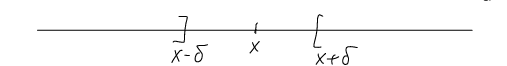
\includegraphics[0.5]{intervalleBoule.png}
       \end{center}
       

   \end{subparag} 
\end{parag}

\begin{parag}{Intérieur d'une boule}
    \begin{definition}
        Soit $E \subset \mathbb{R}^n $ non vide. Alors $ \overline{x} \in E$ est un \important{point intérieur} de $E$ s'il existe $ \delta > 0$ tel que $B( \overline{x}, \delta) \subset E$. L'ensemble des points intérieurs est appelé \important{intérieure} de $E$. Notation $ \mathring{E}$
    \end{definition}
   \begin{subparag}{Remarque personnelle}
       \begin{framedremark}
           On voit ici clairement que $ \mathring{E} < E$. Cette relation est vrai grâce au $ \delta$ qui rend \textit{"plus petit"} notre point $ \overline{x}$
       \end{framedremark}
   \end{subparag}
   Soit $E \subset \mathbb{R}^n $ non vide. Alors $E subset \mathbb{R}^n $ est ouvert $\iff E = \mathring{E}$
   \begin{subparag}{Exemple 1}
       La boule ouverte $B( \overline{x}, \delta) = \{ \overline{y} \in \mathbb{R}^n : \mid  \mid \overline{x} - \overline{y} \mid \mid < \delta \}$ est un sous-ensemble ouvert.\\
       Soit $ \overline{y} \in B( \overline{x}, \delta)$ Alors $ \delta = \frac{1}{2}( \delta - \mid  \mid x - y \mid \mid)  > 0$ implique que:
       \begin{align*}
         &\implies  B( \overline{y}_1, \delta_1) \subset B( \overline{x}, \delta) \\
         &\implies B( \overline{x}, \delta) \subset \mathbb{R}^n 
       \end{align*}
       est un sous-ensemble ouvert de $ \mathbb{R}^n $ $ \forall \overline{x} \in \mathbb{R}^n $, $ \forall \delta > 0$
   \end{subparag}
   \begin{subparag}{Exemple 2}
       Soit $n \geq 2$, $E = \{ \overline{x} \in \mathbb{R}^n  : x_1 = 0, x_i > 0, i = 2, \dots n\} \subset \mathbb{R}^n $
       Ici, nous voulons monter qu'il n'est pas ouvert. \\
       Prenons le point $ \overline{y} = (0, y_2, \dots, y_n)$ où $y_2, \dots, y_n > 0$. Alors pour tout $ \delta > 0$:
       \begin{align*}
           B( \overline{y}, \delta) \ni ( \frac{ \delta}{2}, y_2, \dots, y_n) \notin E
       \end{align*}
       
       
   \end{subparag}
   \begin{subparag}{Exemple 3}
       $\emptyset$ et $ \mathbb{R}^n  \subset \mathbb{R}^n $ sont des sous-ensembles ouverts.      \\
       Ici on a deux cas de figure, 
       \begin{itemize}
           \item $ emptyset$: alors le sous-ensemble est ouvert par définition
           \item Sinon, soit $ \overline{x} \in \mathbb{R}^n $ alors $B( \overline{x}, \delta) \subset \mathbb{R}^n $ et cela: $ \forall \delta > 0$
       \end{itemize}
   \end{subparag}
   \begin{subparag}{Exemple 4}
       $E = \{ \overline{x} \in \mathbb{R}^n: x_i > 0 \forall i = 1, \dots, n\}$\\
       Soit $ \overline{y} \in E$. Alors, nous pouvons prendre $B( \overline{y}, $min$(y_i)) \subset E$.
   \end{subparag}
\end{parag}

\begin{parag}{Propriétés}
    Ici on remarque deux grandes propriétés:
    \begin{enumerate}
       \item Toute réunion $\bigcup_{i \in I} E_i$ des sous-ensembles ouverts est un sous-ensemble ouvert.
           \begin{align*}
               \overline{x} \in \bigcup_{i \in I} E_i \implies \exists j: \overline{x} \in E_j, \; \; E_j \text{ est ouvert } \implies \exists \delta > 0: B( \overline{x}, \delta) \subset E_j \\
               \implies B( \overline{x}, \delta) \subset \bigcup_{i \in I}E_i
           \end{align*}
           

       \item Toute intersection \important{finie} $ \bigcap_{i=1}^nE_i$ des sous-ensembles ouverts est un sous-ensemble ouvert:
            \begin{align*}
               \overline{x} \in  \bigcap_{i\in I}E_i \implies \forall j \overline{x} \in E_j \text{ ouvert } \implies \exists \delta_j > 0 : B( \overline{x}, \delta_j) \subset E_j \\
               \implies B( \overline{x}, \text{min}_j \delta_j) \subset E_j \forall j \implies B( \overline{x}, \text{min} \delta_j) \subset \bigcap_{i=1}^n E_i = E
           \end{align*}
        
    \end{enumerate}
    \begin{framedremark}
        Une intersection infinie des sous-ensembles ouvert de $ \mathbb{R}^n $
    \end{framedremark}
    
\end{parag}



\begin{parag}{Sous-ensemble fermé}
    \begin{definition}
        Soit $E \subset \mathbb{R}^n$ un sous-ensemble. Alors $E$ est \important{Fermé} dans $ \mathbb{R}^n$ si son complément $CE = \{ \overline{x} \in \mathbb{R}^n : \overline{x} \notin E\} = \mathbb{R}^n - E$ est ouvert
    \end{definition}
    
        \begin{align*}
            CB( \overline{x}, \delta) = E \subset \mathbb{R}^n \text{ est fermé}: E = \{ \overline{y} \in \mathbb{R}^n : \mid  \overline{x} - y \mid \geq \delta \} 
        \end{align*}
            Puisque $C(CB( \overline{x}, \delta)) = B( \overline{x}, \delta)$ est ouvert.
\end{parag}
\begin{parag}{Exemples}
    \begin{align*}
        E = \{ \overline{x}\} \subset \mathbb{R}^n 
    \end{align*}
    Ceci est \important{fermé}, car si on prends le complément:
    \begin{align*}
        CE = \{ \overline{y} \in \mathbb{R}^n : \mid \mid \overline{y} - \overline{x} \mid \mid > 0\} \\
        \forall \overline{y} \in CE\; \; \text{la boule} \overline{B}( \overline{y}, \frac{1}{2} \mid  \mid \overline{y} - \overline{x} \mid \mid \subset CE
    \end{align*}
    
    

\end{parag}

\begin{parag}{Question pendant le cours}
    Soient $A$ et $B$ deux sous-ensembles ouverts non-vides de $ \mathbb{R}^n $ Soit $A \setminus B = \{ \overline{x} \in \mathbb{R}^n : \overline{x} \in A \text{ et } \overline{x} \notin B\} $ non-vide.
    \begin{enumerate}
        $A \setminus B$ peut être ouvert, fermé ou ni ouvert ni fermé
        \item $A \setminus$ est soit ouvert, soit fermé
        \item $A \setminus$ ne peut pas être ouvert
        \item $A \setminus$ ne peut pas être fermé
    \end{enumerate}
    Il n'y a qu'une seul possibilité et pour la trouver il faut des contre exemples.

\end{parag}
\begin{parag}{Exemple}
    \begin{align*}
        A = \{(x, y) \in \mathbb{R}^2 : \tan(x + y) \geq 1\}
    \end{align*}
    Et on se pose la question $A$ ouvert, fermé, ni ouvert, ni fermé?
    \\
    Déjà on va trouver tout les valeurs possiblie pour $x$ et $y$ c'est à dire la définition de $\tan$:
    \begin{align*}
        \implies \tan u \text{ existe } \implies u \in ] - \frac{ \pi}{2} + \pi k, \frac{\pi}{2} + \pi k[ \; k \in \mathbb{Z} \\
        \tan u \geq 1 \implies u \in [ \frac{\pi}{4} + \pi k, \frac{\pi}{2} + \pi k[ \; \; \forall k \in \mathbb{Z}
    \end{align*}
   On a donc comme dit auparavant:
   \begin{align*}
       x + y \in  [ \frac{\pi}{4} + \pi k, \frac{\pi}{2} + \pi k[\\
       \frac{\pi}{4} + \pi k \leq x + y < \frac{\pi}{2} + \pi k, k \in \mathbb{Z}\\
       \frac{\pi}{4} + \pi k - x \leq y < \frac{\pi}{2} + \pi k -x
   \end{align*}
   Ici $A$ n'est ni ouvert ni fermé:
   \begin{center}
       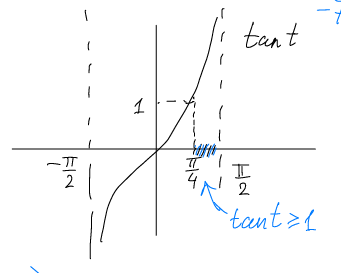
\includegraphics[0.6]{tanBoule.png}
   \end{center}
   \textbf{Explications}: \\
   \begin{enumerate}
       \item $A$ n'est pas ouvert: $(x, y) = (0, \frac{\pi}{4}) = p \in A$
       \begin{align*}
           \forall \delta > 0 \; \; B( \overline{p}, \delta) \text{ contient } (0, \frac{\pi}{4} - \frac{ \delta}{2}) \notin A
       \end{align*}
   \item $A$ n'est pas fermé: $(x, y) = (0, \frac{\pi}{2}) = q \in CA$ 
       \begin{align*}
           \forall \delta > 0 B( \overline{q}, \delta) \text{ contient } (0, \frac{\pi}{2}- \frac{ \delta}{2}) \in A \implies (0, \frac{\pi}{2} - \frac{ \delta}{2}) \notin CA
       \end{align*}
       Et comme $CA$ n'est pas ouvert, alors $A$ n'est pas fermé.
   \end{enumerate}
\end{parag}

\subsection{Méthodes de démonstration: Démonstration par le principe des tiroirs}
\begin{parag}{Principes des tiroirs}
    Si $(n+1)$ objets sont placés dans $n$ tiroirs, alors au moins un tiroir contient $2$ objets ou plus.
    \\
    Plus généralement:
    \begin{theoreme}
        Si $n$ objets sont placés dans $k$ tiroirs, alors au moins un tiroir contient $\left\ceiling \frac{n}{k} \right\ceiling = $min$\{m \in \mathbb{N}: m \geq \frac{n}{k}\}$ objets, ou plus.
    \end{theoreme}
    
    \begin{framedremark}
        Ceci est exactement la même méthode que celle vu en AICC I qu'on appelait le pigeon hole principle, Les preuves sont exactement les mêmes est le but est exactement le même.
    \end{framedremark}
    
\end{parag}


\lecture{8}{2025-02-12}{Suite d'élément de $\mathbb{R}^n$}{}

\begin{parag}{Rappel: Sous-ensembles ouvert et fermmés dans $ \mathbb{R}^n $}
    \begin{definition}
      Soit $E$ un ensemble tel que $E \subset \mathbb{R}^n $ Alors:
      \begin{align*}
          E \subset \mathbb{R}^n  \iff \begin{cases}
              E = \emptyset \\
              E \neq \emptyset \text{et pour chaque point} \overline{x} \in E \text{Il existe} \delta > 0 \text{ tel que } B( \overline{x}, \delta) \subset E
          \end{cases}
      \end{align*}
      
    \end{definition}
    \begin{definition}
        $E \subset \mathbb{R}^n $ est fermé $ \iff$ son complémentaire $CE = \{ \overline{x} \in \mathbb{R}^n : \overline{x} \notin E\}$ est ouvert
    \end{definition}
\end{parag}

\subsection{L'adhérence et la frontière d'un sous-ensemble $ \mathbb{R}^n $}
\begin{parag}{Adhérence}
    \begin{definition}
        Soit $E \subset \mathbb{R}^n $ sous-enesemble non vide. Alors l'intersection de tous les sous-ensembles fermés contenant $E$ est appelée \important{l'adhérence de $E$}.
    \end{definition}
    \begin{subparag}{Notation}
        $ \overline{E}$ est \important{l'adhérence} de $E$ dans $ \mathbb{R}^n $.
        \begin{framedremark}
            Si notre sous-ensemble est déjà fermé alors l'adhérence est égal à lui même:
            \begin{align*}
                E \subset \mathbb{R}^n  \text{fermé} \iff E = \overline{E}
            \end{align*}
            
        \end{framedremark}
        
    \end{subparag}
\begin{definition}
    $E \subset \mathbb{R}^n $ non-vide. $E \neq \mathbb{R}^n $. Un point $ \overline{x} \in \mathbb{R}^n $ est un point de \important{frontière} de $E$ si toute la boule ouverte de centre $x$ cotient au moins un point de  $E$ et au moins un point de $CE$
\end{definition}
L'ensemble des points frontières de $E$ est \important{la frontière de $E$} Notation: $ \partial E$ le d des dérivé partielle.


\end{parag}
\begin{parag}{Exemple}
    \begin{align*}
        E = \{ \overline{x} \in \mathbb{R}^n  : x_i > 0, i = 1, \dots, n\} \implies \partial E = \{ \overline{x} \in \mathbb{R}^n  :  \exists i: x_i = 0, x_j \geq 0 i \neq j\} \\
        \overline{E} = \{ \overline{x} \in \mathbb{R}^n : x_i \geq 0, i = 1, \dots, n\}
    \end{align*}
Soit $E \subset \mathbb{R}^n $ non vide. Alors:
\begin{itemize}
    \item $ \partial E \cap \mathring{E} = \emptyset$
    \item $\mathring{E} \cup \partial E = \overline{E}$ \\
        Ici, on le sait parce que en premier lieu $ \mathring{E} \cup \partial E$ est fermé, et aussi $ E \subset \mathring{E} \cup \partial E$)
    \item $ \partial E = \overline{E} \setminus \mathring{E} = \overline{E} \cup C\mathring{E} \implies \partial E$ est fermé
    \item $ \partial \emptyset = \emptyset$, $ \partial \mathbb{R}^n  = \emptyset$
\end{itemize}
Pourquoi faut il distinguer entre les sous-ensembles ouverts et fermés dans $ \mathbb{R}^n $? La topologie de $ \mathbb{R}^n $ est liée au propriétés des limites des suites d'éléments de $ \mathbb{R}^n $. Et comme la base de l'analyse se base sur la limite, il y a de quoi creuser.

\end{parag}

\subsection{Suites d'éléments de $ \mathbb{R}^n $ et la topologie de $ \mathbb{R}^n $}
\begin{definition}
    \important{Une suite} d'éléments de $ \mathbb{R}^n $ est une application $ f: \mathbb{N} \to \mathbb{R}^n $ 
    \begin{align*}
        f: k \to \overline{x_k} = (x_{1_k}, x_{2_k}, \dots, x_{n_k}) \in \mathbb{R}^n 
    \end{align*}
    Où:
    \begin{align*}
        \{ \overline{x}_k\}_{k=0}^\infty
    \end{align*}
    est une suite d'éléments de $ \mathbb{R}^n $
\end{definition}
\begin{definition}
    $\{ \overline{x}_k\}_{k=0}^\infty$ est \important{convergent} et admet pour \important{limite} $ \overline{x} \in \mathbb{R}^n $ si, pour tout $ \epsilon > 0 \exists k_o \in \mathbb{N}: \forall k \geq k_0, \mid \mid \overline{ \overline{x_k} - \overline{x}} \mid \mid \leq \epsilon$
    Ou alors:
    \begin{align*}
        \overline{x_n} \in \overline{B( \overline{x}, \epsilon} \; \; \forall k \geq k_0
    \end{align*}
    
\end{definition}

\begin{parag}{Remarque}
    soit $ \overline{x} = (x_1, \dots, x_n), \overline{x_k} = (x_{1_k}, \dots, x_{n_k}$, $ \lim_{n \to \infty} \overline{x_k} = \overline{x}$ si et seulement si la limite  $ \lim_{k \to \infty}x_{j_k} = x_j \; \; \forall j= 1, \dots, n$ 

\end{parag}
\begin{parag}{Propriétés}
    \begin{enumerate}
        \item La limite d'une suite $\{ \overline{x}_k\}$, si elle exitste, est unique.
        \item Toute suite convergente $\{ \overline{x_k}\}$ est bornée
            $( \iff $ est contenue dans une boule fermé $ \overline{B( \overline{o}, M)}$
            \begin{align*}
                \lim \overline{x_k} = \overline{x} \implies \exists k_0 \in \mathbb{N}: \forall k \geq k_0 \implies \mid \mid \overline{x} - \overline{x_k} \mid \mid \leq \epsilon \\
                \implies \{ \overline{x_0}, \dots \} \subset \overline{B( \overline{x}, \epsilon)}\\
            \{ \overline{x_0}, \overline{x_1}, \dots, \overline{x}_{k_0-1}\} \cup \{ \overline{x_k}, k \geq k_0\} = \{ \overline{x_k}\}_{k \in \mathbb{N}}
            \end{align*}
            Si nous prenons $M = $ max$\{ \mid \mid \overline{x_i} \mid \mid, i = 0, \dots, k_{o-1}, \mid \mid \overline{x} \mid \mid   + \epsilon\}$
    \end{enumerate}
    

\end{parag}

\begin{parag}{Bolzano-Weierstrass}
    \begin{theoreme}
        De toute suite bornée $\{ \overline{x}_k\} \subset \mathbb{R}^n $ on peut extraire une sous-suite convergente.
    \end{theoreme}
    

\end{parag}
\begin{parag}{Théorème à savoir, Un sous-ensemble non-vide $E \subset \mathbb{R}^n $ est fermé}
\begin{theoreme}
    Un sous-ensemble non vide $E \subset \mathbb{R}^n $ est fermé \important{si et seulement si} toute suite $\{ \overline{x}_k\} < E$ d'élément $E$ qui converge, a pour limite un élément de $E$.
\end{theoreme}
\begin{subparag}{Demonstration $ \implies$ par absurde}
    On cherche dont avec $P$ et $ \neg Q \implies$ absurde
    Soit $ \overline{x} = \lim_{k \to\infty} \overline{x_k}, \overline{x_k} \in E \forall k \in \mathbb{N} $. Supposons par l'absurde que $ \overline{x} \notin E$, $E$ est fermé \\
    ce qui implique que $ \overline{x} \in CE$ où $CE$ est ouvert dans $ \mathbb{R}^n $. Par la définition:
    \begin{align*}
        \exists \delta > 0: B( \overline{x}, \delta) \subset CE \implies \{ \overline{x_k} \forall k \in \mathbb{N}\} \cap B( \overline{x}, \delta) = \emptyset
    \end{align*}
    
    D'autre côté, $ \lim_{k \to \infty} = \overline{x} \implies \exists k_0 \in \mathbb{N}: \forall k \geq k_0, \overline{x}_k \in \overline{B( \overline{x}, \frac{ \epsilon}{2})} \subset B( \overline{x}, \delta)$
\end{subparag}
\begin{subparag}{Contraposé, par contraposé}
    Supposons que $E$ n'est pas fermé, $ \iff$ $CE$ n'est pas ouvert\\
    Alors:
    \begin{align*}
        \implies \exists \overline{y} \in CE \; \forall k \in \mathbb{N}_+ \; \;B( \overline{y}, \frac{1}{k}) \cap E \neq \emptyset\\
        \implies \exists \overline{y_k} \in B( \overline{y}, \frac{1}{k}) \text{ tel que } \overline{y_k} \in E \\
        \text{On a obtenu une suite } \{ \overline{y_k}\}_{k \in \mathbb{N}_+} \subset E \text{ et } \lim_{k \to \infty} \overline{y}_k = \overline{y} \in CE \\
        \iff \overline{y} \notin E\\
        \implies \neq Q \text{ Alors } Q \implies P
    \end{align*}
    

\end{subparag}
\begin{framedremark}
    Pour construire l'adhérence $E$ d'un sous-ensemble non-vide $E \subset \mathbb{R}^n $, il faut et suffit d'ajouter les limites de toues suites convergentes d'éléments de $E$.
\end{framedremark}
    \begin{definition}
        Un sous-ensemble non-vide de $ \mathbb{R}^n $ est \important{compact} s'il est fermé et borné
    \end{definition}
\begin{subparag}{Exemple}
    Soit une boule fermé $ \overline{B( \overline{x}, \delta)} = \{ \overline{y} \in \mathbb{R}^n : \mid \mid \overline{x} - \overline{y} \mid \mid = \delta\}$ Alors $ \overline{B( \overline{x}, \delta)} \subset \overline{B( \overline{o}, \mid \mid \overline{x} \mid \mid+ \delta)}$ est borné. Et donc le sous-ensemble est compact
\end{subparag}
\begin{subparag}{Exemple 2}
    \begin{align*}
        E = \{ \overline{x} \in \mathbb{R}^n : n \geq 2, x_1 = 0\}
    \end{align*}
    est fermé, mais non bornée
    \begin{align*}
        \{ \overline{a}_k = (0, k, 0, \dots)\}_{k \in \mathbb{N}}
    \end{align*}
    Ici les normes $ \mid \mid a_k \mid \mid = k \in \mathbb{N}$. Et donc $CE$ n'est ni borné ni fermé
    
\end{subparag}
\end{parag}
\begin{parag}{Théorème Heine-Borel-Lebesgue}
    \begin{theoreme}
        Un sous-ensemble non-vide $E \subset \mathbb{R}^n $ est compact $ \iff$ de tout recouvrement de $E$ par des sous-ensembles dans $ \mathbb{R}^n $:
        \begin{align*}
            ( E \subset \bigcup_{i \in I} A_i, \; A_i \subset \mathbb{R}^n  \text{ouverts, } A_i \in I \text{ un recouvrement de } E )
        \end{align*}
        On peut extraire une \important{famille finie} d'ensemble que forment un recouvrement de $E$:
        \begin{align*}
            E \subset \bigcup_{i \in I} A_i \; \; A_i \subset \mathbb{R}^n  \text{ ouverts } \implies \exists \{ A_{i_j}\}_{j=1}^m: E \subset \bigcup_{j = 1}^m A_{i_j}
        \end{align*}
    \end{theoreme}
   Ici on peut prendre un nombre infini d'ensemble qui peut recouvrire un nombre fini d'ensemble. Cela ne marche pas si $E$ n'est pas compact.
\begin{subparag}{Exemple 1}
    Une droite dans $ \mathbb{R}^n $, $ n \geq 2$ est fermée, pas bornée $ \implies$ qu'elle n'est pas compacte.
\end{subparag}
\begin{subparag}{Exemple 2}
    Intervalle ouvert dans $  \mathbb{R}$ tel que $E = ] 0, 1 [ \subset \mathbb{R}$ n'est pas fermé ce qui implique que notre ensemble $E$ n'est pas compact
    \begin{align*}
        E \subset \bigcup_{i \in \mathbb{N}} ]0, \frac{i}{i + 1}[
    \end{align*}
    On ne peut pas choisir un sous recouvrement fini. Car si on prends un nombre fini $k$ on dois pouvoir s'arrêter à un $k$ néanmoins ici on n'y arrive pas car on a toujours le nombre $k + 1$
    \begin{framedremark}
        La propriétés d'être compactes est une propriétés très fortes
    \end{framedremark}
\end{subparag}
\end{parag}

\begin{parag}{Exemple}
\begin{subparag}{Exercice}
    \begin{align*}
        A = \{ (x, y) \in \mathbb{R}^2 : \ln (\sin(y-x)) \leq 0\}
    \end{align*}
    Il faut démontrer que $A$ est ouvert.
\end{subparag}
\begin{subparag}{Question 6}
        \begin{align*}
            S = \{ (x, y) \in \mathbb{R}^2: \sqrt{ y \cdot \ln x} < 1\}
        \end{align*}
        \begin{enumerate}
            \item Compact
            \item Ouvert et borné
            \item ni ouvert, ni fermé et non borné
            \item fermé et non borné
            \item ouvert et non borné
            \item ni ouvert, ni fermé et borné
        \end{enumerate}
            
       Pour répondre à cette question, on va prendre tout les cas possibles:
       \begin{enumerate}
           \item $ln x \implies x > 0$
           \item Soit $y = 0 \implies \{ y = 0, x > 0\} \in S$\\
               Aussi $\{ x = 1, y \in \mathbb{R}\} \in S$
           \item Soit $y > 0 \implies y \ln x \geq 0 \implies \ln x geq 0 \wedge x \geq 1$\\
               \begin{align*}
                   y \ln x < 1 \implies y < \frac{1}{\ln x}\\
                   \{y > 0, x > 1, y < \frac{1}{\ln x}\} \subset S
               \end{align*}
           \item Soit $y < 0 \implies y \ln x \geq 0 \implies \ln x \leq 0$ Alors:
               \begin{align*}
                   y \ln x < 1 \implies < \frac{1}{\ln x} \\
                   \{ y < 0, 0 < xx < 1, y > \frac{1}{\ln x}
               \end{align*}
               Ce qui donne comme ensemble:
               \begin{center}
                   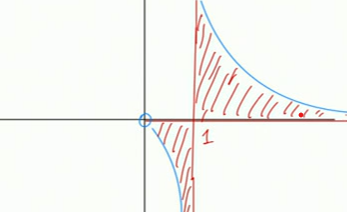
\includegraphics[scale=1.3]{12025-03-12.png}
               \end{center}
               Qui est une droite vertical avec $x = 1$ entre nos deux droite bleu. Néanmoins les lignes bleu ne sont pas inclus, et comme vu sur l'image l'ensemble tends vers les infinis en $x = 1$ et donc, il n'est ni fermé ni borné. Et la raison pour laquelle ce n'est pas ouvert, la  ligne rouge horizontale et fermé et donc ce n'est pas ouvert.
               \begin{framedremark}
                   Attention à faire attention car ici les courbes bleu impliquent que l'ensemble n'est pas fermé mais même si elles étaient fermés, il manquerait quand même le point $0$ qui impliquerait que l'ensemble ne serait pas fermé.
               \end{framedremark}
       \end{enumerate}
\end{subparag}
\end{parag}

\chapter{Fonction réelles de plusieurs variables réelles limite et continuité}
\subsection{Définition et exemples}
\begin{definition}
    Soit $E \subset \mathbb{R}^n $ sous-ensemble non-vide, $n \geq 1$ Une fonction $f : E \to \mathbb{R}$ est une application qui envoie chaque point $ \overline{x} = (x_1, \dots, x_n) \in E$ dans $ \mathbb{R}$. \\
    $E$ est le domaine de définition de $f$ et $f(E)\subset \mathbb{R}$ est l'ensemble image.
\end{definition}
\begin{parag}{Exemple 1}
    \begin{align*}
        f(x, y) = \sqrt{1 - (x^2 - y^2)}
    \end{align*}
    
    
\end{parag}
\begin{parag}{Exemple 2}
    \begin{align*}
        f(x, y) = 2x + 1
    \end{align*}
    Plus généralement:
    \begin{align*}
        f(x, y) = ax + by + c; \; a, b, c, \in \mathbb{R}, E = \mathbb{R}^2
    \end{align*}
  Comment visualiser cette fonction?\\
  \begin{align*}
      \text{Soit } c = 0
  \end{align*}
  Considérons $f(x, y) = ax + by$: Graphique $F = \{(x, y, z): ax + by = z\} = \{(x, y, z) \in \mathbb{R}^3: ax + by -z = 0\} = \{ (x, y, z) \in \mathbb{R}^3: <(x, y, z), (a, b, -1)> = 0\}$ On a donc un plan dont les valeur $a$, $b$ $-1$ sont les composantes d'un vecteur orthogonal: $ \overline{n} = (a, b, -1)$ et contenant $(0, 0, 0)$.
  \\
  Soit $c \in \mathbb{R}$ arbitraire, alors il faut monter le plan par $c$ unité le long de l'axe $z$ pour obtenir le graphique de $f(x, y) = ax+ by + c$ Et donc:
  \begin{align*}
      z = ax + by + x
  \end{align*}
  qui est le plan $ \perp \overline{n} = (a, b, -1)$ qui contient $(0, 0, c)$
  
  
    
\end{parag}
\begin{parag}{Niveau}
    \begin{definition}
        Soit $f : E \to \mathbb{R}$ et $c \in f(E)$ Alors $ \mathcal{N}_f(c) = \{ \overline{x} \in E: f( \overline{x}) = c\} \subset E$
    \end{definition}
    \begin{subparag}{Exemple 4}
        \begin{align*}
            f(x, y) &= \sin(x^2 + y) : E = \mathbb{R}^2\\
            f(E) &= [-1, 1]
        \end{align*}
        
        \begin{framedremark}
            Je conseil de taper sur google les fonctions pour avoir une bonne visualisation de ces fonctions:
            \begin{center}
                \href{https://www.google.com/search?q=sin(x%5E2+%2B+y)&oq=sin(x%5E2+%2B+y)&gs_lcrp=EgZjaHJvbWUyBggAEEUYOTIICAEQABgWGB4yCAgCEAAYFhgeMggIAxAAGBYYHjIICAQQABgWGB4yCAgFEAAYFhgeMgYIBhBFGDwyBggHEEUYPNIBCDM0MDlqMGo0qAIAsAIB&sourceid=chrome&ie=UTF-8}{google.com}
            \end{center}
            
        \end{framedremark}
        On cherche donc les niveaus:
        \begin{align*}
            \mathcal{N}_f(1) &= \{x, y) \in \mathbb{R}^2: \sin(x^2 + y) = 1\}  \\
                             &= \{(x, y) \in \mathbb{R}^2: x^2 + y = \frac{\pi}{2} + 2k\pi, k \in \mathbb{Z}\}\\
                             &= \{(x, y) \in \mathbb{R}^2: y = -x^2 + \frac{\pi}{2} + 2k\pi, k \in \mathbb{Z}
        \end{align*}
        
        
    \end{subparag}

\end{parag}





















\lecture{9}{2025-03-15}{Limite est continuité}{}
\begin{parag}{Rappel}
    \begin{definition}
        Soit $E \subset \mathbb{R}^n $ sous-ensemble non vide, $n \geq 1$ Une fonction est une application qui envoie chaque point $ \overline{x0} = (x_1, \dots, x_n) \in E$ dans $ \mathbb{R}$.\\
        $E$ est le domaine de définition de $f$ et $f(E) \subset \mathbb{R}$ est l'ensemble image.
    \end{definition}
    

\end{parag}

\subsection{Limites et continuité}
\begin{definition}
    Une fonction \important{définie au voisinage de $\overline{x_0}$} (mais pas nécéssairement en $ \overline{x_0}$ tel que
    \begin{align*}
        [ \exists \delta > 0: B( \overline{x}_0, \delta) \subset E \cup \{ \overline{x_0}\}]
    \end{align*}
    admet pour \important{limite} le nombre réel $l$ lorsque $ \overline{x}$ tend vers $ \overline{x_0}$ si \important{pour tout $ \epsilon > 0 \exists \delta > 0$ tel que pour tout $ \overline{x}\in E$ et $0 < \mid \mid \overline{x} - \overline{x}_0 \mid \mid \leq \delta$,  on a $ \mid f( \overline{x}) - l \mid \leq \epsilon$} 
\end{definition}


 \begin{parag}{Notation}
     Pour notre notation on utilise comme à notre habitude:
     \begin{align*}
         \lim_{ \overline{x} \to \overline{x_0}}f( \overline{x}) = l
     \end{align*}
     \begin{framedremark}
         Ici on a la norme $  \mid \mid \overline{x} - \overline{x_0} \mid \mid$ à la place de la valeur absolue lorsqu'on parlait de fonction à une variable. 
     \end{framedremark}
     
 \end{parag}
 \begin{parag}{Continuité}
 
 
 \begin{definition}
     Soit $ \overline{x_0} \in E$ un point intérieur de $E$. Alors $f: E \to \mathbb{R}$ est continue en $ \overline{x} = \overline{x_0}$ \important{si et seulement si}
     \begin{align*}
     \lim_{ \overline{x} \to \overline{x_0}} f( \overline{x}) = f( \overline{x_0})
     \end{align*}
     
 \end{definition}
 

 \begin{subparag}{Exemple 1}
     \begin{align*}
         f(x, y) = 2x + y
     \end{align*}
     soit $(x_0, y0) \in \mathbb{R}^2$: Alors 
     \begin{align*}
         \lim_{(x, y) \to (x_0, y_0)} (x + 2y) = x_0 + 2y_0
     \end{align*}
     Soit $ \epsilon > 0$ alors on cherche $ \mid f(x, y) - f(x_0, y_) \mid = \mid  (x + 2y) - (x_0 + 2y_0) \mid$ si on utilise plus la norme ici et la valeur absolue car on est sur le côté à droite. On utilise l'inéégalité triangulaire:
     \begin{align*}
        &\leq \mid x - x_0 \mid + 2 \mid y - y_0 \mid
     \end{align*}
     Ici on peut toujours prendre comme on a que $ \overline{x} - \overline{x_0}$ plus petit que $ \delta$ on doit les gérer ensembles et non séparément. Des lors:
     Dès lors on choisit $ \delta = \frac{ \epsilon}{3}$
        \begin{align*}
        \leq \sqrt{ (x-x_0)^2 + (y-y_0)^2} + 2\sqrt{(x-x_0)^2 + (y-y_0)^2} = 3\sqrt{(x -x_0)^2 + (y-y_0)^2} \leq 3 \delta = 3 \cdot \frac{ \epsilon}{3} = \epsilon
           \end{align*}

 \end{subparag}
 \begin{subparag}{Exemple 2}
     \begin{align*}
         f(x, y) = x \cdot y \\
         f: \mathbb{R}^2 \to \mathbb{R}
     \end{align*}
     Soit $(x_0, y_0) \in \mathbb{R}^2$ Alors $ \lim_{(x, y) \to (x_0, y_0)} x \cdot y = x_0 \cdot y_0$
     
     \textbf{Démonstration:}\\
    Le cas où $x_0 = 0$ est vu en exercice, dès lors, nous traiterons ici le cas où nous supposerons que $x_0 \neq 0$. Soit $ \epsilon > 0$ alors:
    \begin{align*}
        \mid f(x, y) - f(x_0, y_0)\mid &= \mid xy - x_0y_0 \mid  \\
        &= \mid  (x - x_0)y + x_0(y-y_0) \mid\\
        &\leq \mid x-x_0 \mid \cdot \mid y \mid + \mid y-y_0 \mid \cdot \mid x_0 \mid\\
        \mid y - y_0 \mid \cdot \mid x_0\mid \leq \sqrt{ (x-x_0)^2 + (y-y_0)^2} \mid x_0 \mid \leq  \frac{ \epsilon}{2} \implies \delta \leq \frac{ \epsilon}{2 \mid x_0 \mid} (x_0 \neq 0)\\
        \mid x - x_0 \mid y \mid\mid \leq \sqrt{ (x-x_0)^2 + (y-y_0)^2}\cdot \mid y \mid \leq  \delta  ( \mid y_0 \mid + \delta) \leq \frac{ \epsilon}{2}\\
        \leq \frac{ \epsilon}{2}\\
        \implies \delta \leq \frac{ \epsilon}{2( \mid y_0 \mid + 1)}
    \end{align*}
    On peut choisir comme valeur pour $ \delta$:
    \begin{align*}
        \implies \delta = \text{min} \left( \frac{e}{2 \mid x_0 \mid}, \frac{ \epsilon}{2( \mid y_0\mid + 1)} , 1 \right)  \implies \mid f(x, y)  f(x_0, y_0) \mid \leq \frac{ \epsilon}{2} + \frac{ \epsilon}{2} = \epsilon
    \end{align*}
    
    
     
 \end{subparag}
 \end{parag}

 \begin{parag}{Caractérisation de la limite à partir des suites convergentes}
     \begin{theoreme}
         Une fonction $f: E \to \mathbb{R}$ définie au voisinage de $ \overline{x_0}$ admet pour limite $l \in \mathbb{R}$ lorsque $ \overline{x} \to \overline{x_0}$  \important{Si et seulement si} pour toute suite d'élément $\{ \overline{a_k}\}$ de $\{ \overline{x} \in E: \overline{x} \neq \overline{x_0}\}$, qui converge vers $ \overline{x_0}$, la suite $\{f( \overline{a}_k)\}$ converge vers $l$.
         \begin{align*}
             \lim_{ \overline{x} \to \overline{x_0}} f( \overline{x}) = l \iff \lim_{ k \to \infty} f( \overline{a_k}) = l \text{ pour toute suite } \{ \overline{a_k}\} \subset E \setminus \{ \overline{x_0}\}: \lim_{k \to \infty} \overline{a_k} = \overline{x_0}
         \end{align*}
     \end{theoreme}
 \end{parag}
 
 \begin{parag}{Démonstration}
     \begin{subparag}{ $ \implies$ $P \implies Q$}
         Comme ce théorème est une équivalence, nous allons devoir prouver les deux sens. Commençons par $P \implies Q$. Prenons la définition de la limite à gauche:
         \begin{align*}
             &\lim_{ \overline{x} \to \overline{x_0}} f( \overline{x})= l \implies \forall \epsilon > 0 \exists \delta > 0: \forall \overline{x}: 0 < \mid \mid \overline{x} - \overline{x_0} \mid \mid \leq \delta\\
             &\implies \mid f( \overline{x}) - l \mid \leq \epsilon \\
             &\text{Si on a } \{ \overline{a_k}\}: \lim_{k \to \infty} \overline{a_k} = \overline{x_0} \implies \text{  pour } \delta > 0 \exists k_0 : \forall k \geq k_0 \\
             &\implies \mid \mid \overline{a_k} - \overline{x_0} \mid \mid \leq \delta \implies \mid f( \overline{a_k}) - l \mid \leq \epsilon \\
             &\mid  f( \overline{a}_k) - l \mid \leq \epsilon
         \end{align*}
         \begin{framedremark}
             L'idée ici est de prendre le même $ \delta$ sur les deux première lignes.
         \end{framedremark}
         
     \end{subparag}
     \begin{subparag}{$(\impliedby)$ par contraposée}
         Petit rappel pour la contraposée: si on a $ Q \implies P$ alors la contraposé est $ \neg P \implies \neg Q$ donc ici on veut prouver que si la limite n'est pas $l$ alors la limite de $f( \overline{a_k})$ n'est pas non plus $l$.\\
         Supposons donc que $\lim_{ \overline{x} \to \overline{x_0}}f( \overline{x}) \neq l $ Alors:
             \begin{align*}
                 \exists \epsilon > 0: \forall \delta > 0 \exists \overline{x}_\delta: \mid \mid \overline{x_k} - \overline{x_0} \mid \mid \leq \frac{1}{ \delta} \mid \text{ et } \mid f( \overline{x}_\delta) - l \mid > \epsilon
             \end{align*}
             Dès lors, on peut choisir $ \delta = \frac{1}{k}$, $k \in \mathbb{N}^*$  ce qui implique:
             \begin{align*}
                 \exists \overline{x}_k \in E : \mid \mid  \overline{x_k} - \overline{x_0} \mid \mid \leq \frac{1}{k} \text{ et } \mid f( \overline{x_k}) - l \mid > \epsilon
             \end{align*}
             On obtient la suite $\{ \overline{x}_k\}_{k=1}^\infty: \lim_{k \to \infty} \overline{x_k} = \overline{x_0}$ mais $ \mid f( \overline{x_k}) - l \mid > \epsilon \forall k \in \mathbb{N}^*$ Dès lors
             \begin{align*}
                 \implies f( \overline{x}_k) \neq l
             \end{align*}
     \end{subparag}

     \begin{subparag}{Idée générale de la preuve}
         Ici on prends $P$ et \important{Ensuite} $\neg P$ il est important de pouvoir différencier les deux et de pouvoir construite $\neg P$ à partir de $P$.
         
     \end{subparag}
 \end{parag}

 \begin{parag}{Opération algébrique}
     Soit $f, g$ deux fonctions: $ E_{ \mathbb{R}^n } \to \mathbb{R}$ telles que $\lim_{ \overline{x} \to \overline{x_0}}f( \overline{x}) = l_1$ et $\lim_{ \overline{x} \to \overline{x_0}}g( \overline{x}) = l_2$ Alors:
     \begin{enumerate}
         \item $\lim_{ \overline{x} \overline{x_0}} ( \alpha f + \beta g)( \overline{x}) = \alpha l_1 + \beta l_2$
         \item $\lim_{ \overline{x} \to \overline{x_0}} (f \cdot g)( \overline{x}) = l_1 \cdot l_2$ 
         \item Si $l_2 \neq 0$, alors $\lim_{ \overline{x} \to \overline{x_0}}( \frac{f}{g})( \overline{x}) = \frac{l_1}{l_2}$
     \end{enumerate}
    \begin{subparag}{Conclusion}
        Tous les polynômes en plusieurs variables et toutes les fonctions rationnelles sont continues sur leur domaines de définition,
        \begin{framedremark}
            La caractérisation de la limite à partir des suites convergentes est pratique pour montrer qu'une fonction n'admet pas de limite en $ \overline{x_0} \in \mathbb{R}^n $.
        \end{framedremark}
    \end{subparag} 
    \begin{subparag}{Exemple 1}
        \begin{align*}
            f: \mathbb{R}^2 \to \mathbb{R}\\
            f(x, y) = \begin{cases}
                \frac{xy}{x^2 + y^2} \text{ si } (x, y) \neq (0, 0)\\
                0 \text{ si } (x, y) = (0, 0)
            \end{cases}
        \end{align*}
        Soit $ \overline{a_k} = ( \frac{1}{k}, \frac{1}{k}) \to (0, 0)$ qui implique donc pour la limite:
        \begin{align*}
            \lim_{ k \to \infty} f( \overline{a_k}) = \lim_{k \to\infty} \frac{ \frac{1}{k} \cdot \frac{1}{k}}{ \frac{1}{k^2} + \frac{1}{k^2}} = \frac{1}{2}
        \end{align*}
        Dès lors, on peut aussi prendre $ \overline{b_k} = ( \frac{1}{k},0) \to (0, 0)$ qui par le même procédé:
        \begin{align*}
            \lim_{k \to \infty} f( \overline{b_k}) = \lim_{k \to \infty} \frac{ 0 \cdot \frac{1}{k}}{0 + \frac{1}{k^2}} = 0
        \end{align*}
        Et donc, par la caractérisation à partir des suites, $\lim_{(x, y) \to (0, 0)} f(x, y)$ ne peut pas exister.\\
        On peut aussi prendre une autre suite du genre $ \overline{c_k} = ( - \frac{1}{k}, \frac{1}{k}) \implies \lim_{k \to \infty} f( \overline{a_k}) = - \frac{1}{2}$\\
        Alors quelle est la limite $f(x, y)$ en $(0, 0)$
         \begin{center}
     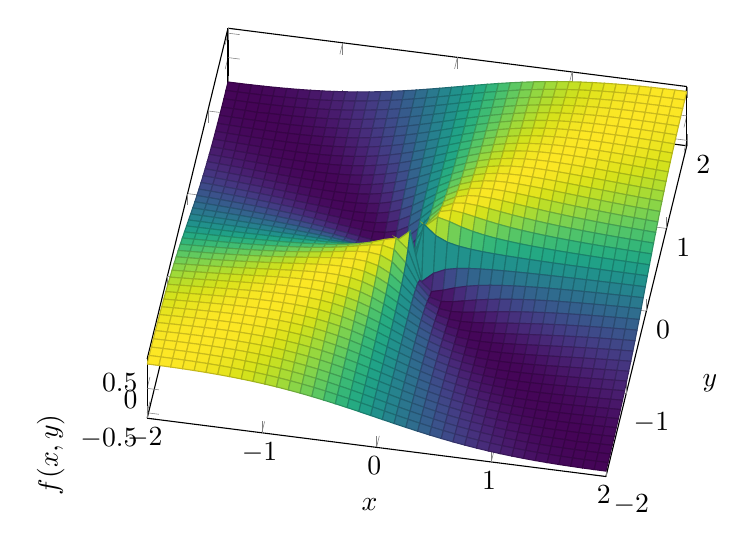
\begin{tikzpicture}
         \begin{axis}[
         view={10}{80},
         domain=-2:2,
         y domain = -2:2,
         colormap/viridis,
         xlabel={$x$},
         ylabel={$y$},
         zlabel={$f(x, y)$},
         samples=40,
         samples y=40,
         ]
         \addplot3[surf] {x*y/(x^2 + y^2)};
     \end{axis}
     \end{tikzpicture}
     
     
 \end{center}
 
    \end{subparag}
    \begin{subparag}{Proposition}
        \begin{theoreme}
            soir $D \subset \mathbb{R}^n $, $f: D \to \mathbb{R}$ définie au voisinage de $ \overline{x_0} \in \mathbb{R}^n $. Alors $\lim_{ \overline{x} \to \overline{x_0}}f( \overline{x}) =l$ si et seulement si pour toute courbe $ y: [a, b] \to \mathbb{R}^n $ telle que:
            \begin{align*}
                 \Upsilon([a, b]) \subset D \setminus\{ \overline{x_0}\} \text{ et } \lim_{t \to a^*} y(t) = \overline{x_0}, \text{ on a } \lim_{t \to a^+} f(y(t)) = l
            \end{align*}
           
        \end{theoreme}
       \begin{framedremark}
           On ne peut pas calculer la limite d'une fonction de plusieurs variable en faisant de manière consecutive par rapport à chaque variable.

       \end{framedremark}
        
    \end{subparag}

    \begin{subparag}{Exemple 2}
        \begin{align*}
            f(x, y) = \begin{cases}
                \frac{x^2 - y^2}{x^2 + y^2} \text{ si } (x, y) \neq (0, 0)\\
                0 \text{ si } (x, y) = (0, 0)
            \end{cases}
        \end{align*}
        Alors on prends deux fonctions;:
        \begin{align*}
            y_1(t) = (t, 0)\\
            y_2(t) = (0, t)
        \end{align*}
        \begin{align*}
            \lim_{t \to o}( \gamma_1(t)) = \lim_{t \to o} \frac{t^2 - 0}{t^2 + 0} = 1\\
            \lim_{t \to 0}f( \gamma_2(t)) = \lim_{t \to 0} \frac{0 - t^2}{0 + t^2} = -1
        \end{align*}
       Et donc la fonction n'a pas de limite en ce point.
    \end{subparag}
    \begin{subparag}{Exemple 3}
        soit:
        \begin{align*}
            f: \mathbb{R}^2 \to \mathbb{R}\\
            f(x, y) = \begin{cases}
                \frac{x^3 + y^3}{x^2 + y^2}\\
                0
            \end{cases}
        \end{align*}
        En prenant les mêmes fonctions:
        \begin{align*}
            \gamma_1(t) = (t, 0) \implies \lim_{t \to 0} \gamma_1(t) = \overline{0}, \lim_{t \to 0} \frac{t^3 + 0}{t^2 + 0} = 0\\
            \gamma_2(t) = (0, t) \implies \lim_{ t \to 0} \gamma_2(t) = \overline{0}, \lim_{t \to 0} \frac{0 - t^3}{0 + t^2} = 0\\
                    \gamma_3 (t, t) \implies\lim_{t \to 0} \gamma_3(t) = \overline{0}, \lim_{t \to 0} \frac{t^3 + t^2}{t^2 + t^1} = 0
        \end{align*}
       On voit ici que ces fonctions ont toute la même limite, et si on prenait n'importe quelle autre  fonction la limite existerait toujours.
       \textbf{Hypothèse} $\lim_{(x, y) \to (0, 0)} f(x, y) = \overline{0}$
    \end{subparag}
 \end{parag}
 
 \begin{parag}{Méthode de changement de variables polaires}
     On peut démontrer l'existence de cette limite par le changement de variables en coordonnées polaires.:
     \begin{align*}
         x = r\cos \phi \text{ si } r \in \mathbb{R}_{ \geq 0}\\
         y = r\sin \phi \text{ si } r \neq 0
     \end{align*}
     Alors on a:
     \begin{align*}
         f(x, y) &= \frac{x^3 + y^3}{x^2 + y^2} \implies f(r, \phi) = \frac{r^3\cos^3\phi + r^3\sin^3\phi}{r^2\cos^2\phi + r^2\sin^2\phi}\\
         &= \frac{r^2(cos^3\phi + \sin^3\phi)}{r^2}\\
         &= r(cos^3\phi + \sin^3\phi)
     \end{align*}
     Ici, $\phi(r)$ est une fonction inconnue, elle pourrait être n'importe quoi.
     \begin{align*}
         \lim_{(x, y) \to (0, 0)}f(x, y) = \lim_{r \to 0} \Phi(r, \phi)\\
         \lim_{r \to 0}\mid r (cos^3\phi + \sin^3\phi) \mid = 0\\
         \implies \lim_{(x, y) \to (0, 0)} f(x, y) = 0
     \end{align*}
     
     
     \begin{framedremark}
         Cette méthode est efficace pour montrer l'existence des limites pour des fonctions de seulement deux variables, et qui tendent vers $(0, 0)$ tel que $\lim_{(x, y) \to (0, 0)} f(x, y)$
     \end{framedremark}
     
     
 
 \end{parag}
\begin{parag}{Théorème des $2$ gendarme}
    \begin{theoreme}
        Soit $f, g, h: E^{\subset \mathbb{R}^n } \to \mathbb{R}$ telles que:
        \begin{enumerate}
            \item $\lim_{ \overline{x} to \overline{x_0}}f( \overline{x}) = \lim_{ \overline{x} \to \overline{x_0}} g( \overline{x}) = l$
            \item Il existe $ \alpha > 0$ pour tout $x \in \{ x \in E: o < \mid \mid \overline{x}- \overline{x_0} \mid \mid \leq \alpha\}$ on a:
                \begin{align*}
                    f( \overline{x}) \leq h( \overline{x}) \leq g( \overline{x})
                \end{align*}
       Alors:
       \begin{align*}
           \lim_{ \overline{x} \to \overline{x_0}}h( \overline{x}) = l
       \end{align*}
        \end{enumerate}
    \end{theoreme}
    
\end{parag}
 
\begin{parag}{Critère des $2$ gendarmes en coordonnées polaires}
    \begin{subparag}{Proposition}
        Soit $D \subset \mathbb{R}^2, f: D \to \mathbb{R}$ définie au voisinage de $(x_0, y0) \in \mathbb{R}^2$. \\
        Alors
        \begin{align*}
            \lim_{(x, y) \to (x_0, y_0)} f(x, y) = l \text{ si et seulement si}
        \end{align*}
      \begin{align*}
          \exists \delta > 0 \text{ et } \phi: ] 0 , \delta [ \to \mathbb{R}:
      \end{align*}
    \begin{itemize}
        \item $ \forall \phi \in [0, 2\pi] \implies \mid f(x_0, r\cos\phi, y_0 + r\sin\phi) - l \mid \leq \phi(r)$
        \item $\lim_{r \to o^+} \phi(r) = 0$
    \end{itemize}    
    \end{subparag}

    \begin{subparag}{Exemple 5}
       soit 
       \begin{align*}
           f(x, y) = \begin{cases}
               \frac{4xy^2}{x^2 + y^2 + 3y^4} \\
               0
           \end{cases}\\
           f(r\cos\phi, r\sin\phi) = \frac{4r^3\cos\phi\sin^2\phi}{r^2 + 3r^4\cos^4\phi} = \frac{4r^3\cos\phi\sin^2\phi}{r^2(1 + 3r^2\sin^4\phi}\\
           \mid f(r\cos\phi, r\sin\phi) - 0 \mid = \frac{4r^3 \mid \cos\phi\sin^2\phi \mid}{r^2 \mid 1 + 3r^2\sin^4\phi \mid}
       \end{align*}
       On sait ici que la partie du nominateur (la partie en haut j'ai un doute) est toujours plus petite ou égale à 1 et la partie du bas plus grande ou égal à $1$. ce qui nous donne:
       \begin{align*}
           \leq \frac{4r^3}{r^2} = 4r = \Phi(r)
       \end{align*}
       Alors 
        \begin{align*}
            \lim_{r \to 0} \Phi(r) = 0
        \end{align*}
        Ce qui par les $2$ gendarmes en coordonnées polaires nous donne:
        \begin{align*}
            \lim_{(x, y) \to (0, 0)} f(x, y) = (0, 0)
        \end{align*}
    \end{subparag}
\end{parag}
\begin{parag}{Question à la fin du cours (Question 7)}
Soit les fonctions \begin{align*}
    f(x, y) = \begin{cases}
        \frac{cos(xy)(x^2 + \sin(y^2))}{\sqrt{x^2 + y^2}}, \; (x, y) \neq (0, 0)\\ 
        0 , \; \text{ Autrement}
    \end{cases} \\
    g(x, y) = \begin{cases}
        \frac{x^2 + y^4}{y^2 + x^4 + x^6}, \; \text{ si } (x, y) \neq (0, 0)\\
        0, \text{ autrement}
    \end{cases}
\end{align*}
La question est quelle fonction est continue en $(0, 0)$?
\begin{subparag}{Solution $f(x, y)$}
    On passe d'abord en coordonnées polaire:
    \begin{align*}
        f(r\cos\phi, r\sin\phi) = \frac{\cos(r^2\sin\phi\cos\phi)(r^2\cos\phi + \sin(r^2\sin^2\phi))}{r}
    \end{align*}
    On prend ensuite la limite:
    \begin{align*}
        \mid f(r\cos\phi, r\sin\phi) - 0 \mid &= \frac{ \mid \cos(r^2\sin\phi\cos\phi) \mid \mid r^2\cos\phi + \sin(r^2\sin^2\phi) \mid}{r}\\
                                              &\leq \frac{ \overbrace{r^2\cos\phi}^{ \geq r^2} + \mid \overbrace{\sin(r^2\sin^2\phi)}^{\leq \mid r^2\sin^2\phi \mid \leq r^2} \mid}{r}\\
                                              &\leq \frac{2r^2}{r} = 2r
    \end{align*}
    Et donc ici on voit que la limite de la fonction va bien vers $0$. ON peut aussi le \textit{"deviner}" en voyant un $r$ tout seul en bas et une $r^2\cos \dots$ en haut. Cela peut donner quelque indice.
\end{subparag}
\begin{subparag}{Solution $g(x, y)$}
    Pour cette fonction on refait le même procédé mais avant on va tester les limites du type $\lim_{t \to 0}g(0, t)$ et aussi $\lim_{t \to 0}g(t, 0)$ et on voit qu'elle ne donne pas la même réponse et que donc, la limite n'existe pas. 
    
\end{subparag}
\end{parag}


 
 
        

\lecture{10}{2025-03-19}{Limites de fonctions}{}
\begin{parag}{Rappel}
    Voici un petit tappel sur les méthodes de calcul des limites de fonction $f: E_{ \subset \mathbb{R}^2} \to \mathbb{R}$
    \begin{enumerate}
        \item s'il existent $2$ suites $ \overline{a_k}$ et $ \overline{b}_k \subset E \setminus\{ \overline{x_0}\}: \lim_{ k \to \infty} \overline{a_k} = \overline{x_0}, \lim_{k \to \infty} \overline{a_k} = \overline{x_0}$ et que, $\lim_{k \to \infty}f( \overline{a_k}) \neq \lim_{k \to \infty} f( \overline{b_k})$ Alors la limite
            \begin{align*}
                \lim_{ \overline{x} \to \overline{x_0}} f( \overline{x})
            \end{align*}
            n'existe pas
        \item S'il existent $2$ courbe $ \gamma_1, \gamma_2: [a, b] \to E \setminus \{ \overline{x_0}\}$ tel que:
            \begin{align*}
                \lim_{t \to a^+} \gamma_1(t) = \lim_{ t \to a^+} \gamma_2(t) = \overline{x_0}
            \end{align*}
            Et que:
            \begin{align*}
               \lim_{t \to a^+}f( \gamma_1(t)) \neq \lim_{t \to a^+} f( \gamma_2(t))
            \end{align*}
            Alors, la limite $ \lim_{ \overline{x} \to \overline{x_0}}f( \overline{x})$ n'existe pas. 
        \item Deux gendarmes: soit $f, g, h: E \to \mathbb{R}$ telles que 
            \begin{align*}
                    \lim_{ \overline{x} \to \overline{x}_0} f( \overline{x}) = \lim_{ \overline{x} \to \overline{x}_0} g( \overline{x})= l
            \end{align*}
            Et que $ \exists \alpha > 0:\; \forall x \in \{x \in E: 0 < \mid \mid \overline{x}- \overline{x_0} \mid \mid < \alpha\}$ on a
            \begin{align*}
                f( \overline{x}) \leq h( \overline{x}) \leq g( \overline{x})
            \end{align*}
            Alors, $h( \overline{x}) = l$
        \item Coordonnées polaires: $f: E \to \mathbb{R}$. Alors $ \lim_{r \to o} f( r\cos\phi, r\sin\phi) = 0 \iff \lim_{(x, y) \to (0, 0)} f(x, y) = 0$ 
            \important{Ici $\phi = \phi(r)$ est une fonction inconnue de $r$}
        \item Deux gendarmes en coordonnées polaires: $f: E \to \mathbb{R}$\\
           \begin{align*}
               \lim_{(x, y) \to (0, 0)} f(x, y) = l \iff \exists \delta > 0 \text{ et } \Phi : ]0, \delta[ \to \mathbb{R}\\
               \forall \phi \in [0, 2\pi], \; \; \forall r \in ]0, \delta [ \text{ on a } \mid f(r\cos\phi, r\sin\phi) - l \mid \leq \Phi(r) \\
               \text{ et } \lim_{r \to o^+} \Phi(r) = 0
           \end{align*}
    \end{enumerate}
    

\end{parag}

\begin{parag}{Développement limité}

    Pour calculer des limites, on peut aussi utiliser les DL connus pour les fonctions d'une seule variables pour trouver des estimations pour les deux gendarme.\\
    Notemment, dans les limites lorsque $ \mid \mid (x, y) - (0, 0) \mid \mid \to 0$ on peut remplacer des expression $\Phi(x)$, $\phi(x)$ par leur DL autour de $x = 0$ ou $y = 0$:
    \begin{align*}
        \Phi(t) = \sum_{k= 0}^n a_\alpha x^k + x^n \cdot \epsilon(x) \text{ 1 seule variable}\\
        x(y) = \sum_{k=0}^n b_k y^k + y^n \cdot \epsilon(y), \dots
    \end{align*}
   On peut composer une fonction d'une seule variable 
   \begin{subparag}{Proposition}
       oit $D \subset \mathbb{R}^2, \: (x_0, y_0) \in D, g:D \to \mathbb{R}$ définie au voisinage de $(x_0, y_0)$, telle que 
       
   \end{subparag}
\end{parag}



\lecture{11}{2025-03-24}{Differentiable}{}


\begin{parag}{Méthode $7$ Récurrence}
    \begin{subparag}{Le principe fondamental de récurrence}
        Soit $S \subset \mathbb{N}$ sous-ensemble : $ 0 \in S$ et pour tout $n \in S$ on a $(n+1) \in S$. Alors $S = \mathbb{N}$
    \end{subparag}
    \begin{subparag}{Méthode de récurrence}
        Soit $P(n)$ une proposition qui dépend de $n \in \mathbb{N}$, $n \geq n_0$\\
Supposons que
        \begin{itemize}
            \item $P(n_0)$ est vraie
            \item $P(n)$ implique $P(n+1)$ pour tout $n \geq n_0$ naturel
        \end{itemize}
        Alors $P(n)$ est vraie pour tout $n \geq n_0$
    \end{subparag}
On regroupe quatre étapes pour une preuve par récurrence:
\begin{enumerate}
\item La proposition ( Soit $P(n)$ la proposition pour $x$)
\item L'initialisation $P(0)$
\item L'hérédité: Supposons que $P(n)$ est vrai, alors il faut en déduire $P(n+1)$
\item Conclusion: Puisque $P(x_0)$ est vraie et que pour tout $x \geq x_0$, $P(n) \implies P(n+1)$, par récurrence $P(n)$ est vraie $ \forall n \geq x_0$. 
    
\end{enumerate}
\begin{framedremark}
    Attention a ne pas mélanger ce qu'on veut et ce qu'on a.
\end{framedremark}

\end{parag}
\begin{parag}{Récurrence généralisée}
    Soit $P(n)$ une proposition qui dépend de $n \in \mathbb{N}, n \geq n_0$.\\
    Supposons que $(1) P(n_0), \dots P(n_0 + k)$ sont vraie pour un $k \in \mathbb{N}$\\
    En deuxième $\{ P(n), P(n+1), \dots, P(n+k)\}$ impliquent $P(n +k+1) \forall n \geq n_0$, $n \in , \mathbb{N}$.\\
    Alors, $P(n)$ est vraie $ \forall n \geq n_0$, $ n \in \mathbb{N}$
\end{parag}

\chapter{Calcul différentielle des fonctions de plusieurs variables}

    \section{Dérivées parielles, le gradient}
    \begin{parag}{Dérivée partielle}
        \begin{definition}
            Soit $f : E \to \mathbb{R}$ une fonction, $E \subset \mathbb{R}$ sous-ensemble ouvert. \\
        Soit $g(s) = f(a_1, a_2, \dots, \overbrace{s}^{k}, a_{k+1}, \dots, a_n)$ où $ \overline{a} = (a_1, \dots, a_n) \in E$.
        \begin{align*}
            g: D = \{ s \in \mathbb{R} : (a_1, a_2, \dots, s, a_{k+1}, \dots, a_n) \in E\} \to R
        \end{align*}
        Alors si $g$ est dérivable en $a_k \in D$, on dit que la \important{k-ième dérivée partielle} de $f$ en $ \overline{a} \in E$ existe et est égale à $g'(a_k)$
        \begin{framedremark}
            Notation: $ \frac{ \partial f}{ \partial x_k}( \overline{a}) \equiv D_k f( \overline{a})$
        \end{framedremark}
        \end{definition}
        
       On a:
        \begin{align*}
            \frac{ \partial f}{ \partial x_k} ( \overline{a}) = \lim_{ t \to 0} \frac{g(a_k + t) - g(a_k)}{t} = \lim_{t \to 0} \frac{f( \overline{a} + t \overline{e_k}) - f( \overline{a})}{t}
        \end{align*}
      
    \end{parag}
    
   \begin{parag}{Gradient}
       \begin{definition}
           Si toutes les dérivées partielles existent en $ \overline{a} \in E$: $ \frac{ \partial f}{ \partial x}( \overline{a})  \dots \frac{ \partial f}{ \partial x_n}( \overline{a})$, alors on définit le \important{gradient} de $f$ en $ \overline{a}$ comme:
           \begin{align*}
             \nabla  f( \overline{a}) = \left( \frac{ \partial f}{ \partial x}( \overline{a}), \dots \frac{ \partial f}{ \partial x_2}( \overline{a}) , \dots\frac{ \partial f}{ \partial x_n}( \overline{a}) \right) 
           \end{align*}
           
       \end{definition}
   
   \end{parag}
    
       \section{Dérivée directionnelle}
       \begin{parag}{Définition}
           Soit $E \subset \mathbb{R}^n $ sous-ensemble ouvert, $ \overline{a} \in E$, $\overline{v} \in \mathbb{R}^n , \overline{v} \neq 0$ La droite passant par $ \overline{a}$ en direction $ \overline{v}$ admet la paramétrisation $ \overline{e}(t) = \overline{a}  + t \overline{v}$ et cela $ \forall t \in \mathbb{R}$.\\
           Considérons la fonction $ f : E \to \mathbb{R}$\\
           et soit $g(t) = f( \overline{a} + t + \overline{v})$ la fonction d'une seule variable $t \in \mathbb{R}$:
           \begin{align*}
               g: D = \{t \in \mathbb{R}: \overline{a} + t \overline{v} \in E\} \to R
           \end{align*}
           \begin{definition}
               Si $g$ est dérivable en $t = 0$ on dit qu'il existe \important{la dérivée directionnelle} de $f$ en $ \overline{a}$ suivant le vecteur $ \overline{v}$ (en direction de $\overline{v}$)\\
               La dérivée directionnelle de $f$ en $ \overline{a}$ en direction de $ \overline{v}$ est:
               \begin{align*}
                   Df( \overline{a}, \overline{v}) = \frac{\partial f}{\partial \overline{v}}( \overline{a}) = \lim_{t \to 0} \frac{g(t) - g(0)}{t} = \lim_{t \to 0} \frac{f( \overline{a} + t \overline{v}- f( \overline{a}}{t}
               \end{align*}
               
           \end{definition}
           
       \begin{framedremark}
           Si $ \overline{v} = \overline{e}_i$ ou $ \overline{e_i}$ est un vecteur unitaire, Alors \begin{align*}
              Df( \overline{a}, \overline{e}_i) = \frac{\partial f}{\partial x_i}( \overline{a})
           \end{align*}
           Si toutes les dérivées directionnelles existent en $ \overline{a}$ (pour tout $ \overline{v} \neq \overline{0}$), alors toutes les dérivées partielles existent en $ \overline{a}$. La réciproque est fausse en générale
       \end{framedremark}
         \begin{framedremark}
             \begin{align*}
                 Df( \overline{a}, \lambda \overline{v}) = \lambda \cdot Df( \overline{a}, \overline{v}) \;\; \forall \lambda \in \mathbb{R}: \; \lambda \neq 0
             \end{align*}
             
         \end{framedremark}
           
       
       \end{parag}
       
       
           \section{Dérivabillité et la différentielle}
           \begin{definition}
               Soit $f: E \to \mathbb{R}$, $E \subset \mathbb{R}^n $ ouvert, $ \overline{a} \in E$\\
               On dit que $f$ est \important{dérivable} au point $ \overline{a}$ s'il existe une transformation linéaire:
               \begin{align*}
                   L_{ \overline{a}}: \mathbb{R}^n  \to \mathbb{R}
               \end{align*}
               et une fonction $ r: E \to \mathbb{R}$ telle que:
               \begin{align*}
                   f(x) = f( \overline{a}) + L_{ \overline{a}}( \overline{x} - \overline{a}) + r ( \overline{x}) \; \; \forall \overline{x} \in E\\
                   \lim_{ \overline{x} \to \overline{a}} \frac{r( \overline{x})}{ \mid \mid \overline{x} - \overline{a} \mid \mid}
               \end{align*}
           \end{definition}
           \begin{definition}
               $L_{ \overline{a}}$ s'appelle \important{la différentielle} de $f$ au point $ \overline{a} \in E$\\
Notation:
\begin{align*}
    L_{ \overline{a}} = df( \overline{a})
\end{align*}

           \end{definition}
           \begin{framedremark}
               Une transformation linéaire $ T: \mathbb{R}^n  \to \mathbb{R}$ est une fonction telle que $\tau ( \alpha \overline{x}_1 + \beta \overline{x}_2) = \alpha T( \overline{x}_1) + \beta T( \overline{x}_2)$ pour tout $ \overline{x}_1, \overline{x}_2 \in \mathbb{R}^n $
Par example $x + 3y$ est une transformation linéaire tandis que $ x + 2y + 2$ n'en est pas une.
               
           \end{framedremark}
           
           

\lecture{12}{2025-03-26}{Tangente de la surface}{}
\begin{parag}{Rappel}
    \begin{definition}
        Soit $f: E \to \mathbb{R} , \; E \subset \mathbb{R}^n $ ouvert, $a \in E$.\\
        On dit que $f$ est dérivable au point $ \overline{a}$ s'il existe une transformation linéaire $L_{ \overline{a}}: \mathbb{R}^n  \to \mathbb{R}$ et une fonction $r: E \to \mathbb{R}$ telles que:
        \begin{align*}
            f( \overline{x}) = f( \overline{a}) + L_{ \overline{a}}( \overline{x} - \overline{a}) + r( \overline{x}) \; \forall \overline{x} \in E\\
            \lim_{ \overline{x} \to \overline{a}} = \frac{r( \overline{x})}{ \mid \mid \overline{x} - \overline{a}\mid \mid} = 0
        \end{align*}
        
    \end{definition}
    

\end{parag}

\begin{parag}{Théorème $1$}

    \begin{theoreme}
        Soit $f: E \to \mathbb{R}$, $ \overline{a} \in E$ tel que $f$ est dérivable en $ \overline{a}$ de différentielle $L_{ \overline{a}}: \mathbb{R}^n \to \mathbb{R}$. Alors:
        \begin{itemize}
            \item $f$ est continue en  $\overline{a} \in E$
            \item Pour tout $\overline{v} \in \mathbb{R}^n , \overline{v} \neq \overline{0}$, la dérivée directionnelle $Df( \overline{a}, \overline{v})$ existe et 
                \begin{align*}
                    Df( \overline{a}, \overline{v}) = L_{ \overline{a}}( \overline{v})
               \end{align*}
           \item Toutes les dérivées partielles existent de $f$ en $\overline{a}$ et
               \begin{align*}
                   \frac{\partial f}{\partial x_k}( \overline{a}) = L_{ \overline{a}}( \overline{e}_k)
               \end{align*}
               Le gradient de $f$ existent en $ \overline{a}$ et:
               \begin{align*}
                   \nabla f( \overline{a}) = \left( L_{ \overline{a}}( \overline{e_1}),  L_{ \overline{a}}( \overline{e_2}), \dots,  L_{ \overline{a}}( \overline{e_n}) \right)
               \end{align*}
           \item Pour tout $\overline{v} \in \mathbb{R}^n $, $ \overline{v} \neq \overline{0}$
               \begin{align*}
                   Df( \overline{a}, \overline{v}) = L_{ \overline{a}}( \overline{v}) = < \nabla f( \overline{a}), \overline{v}>
               \end{align*}
           \item Pour tout $ \overline{v} \in \mathbb{R}^n $, $ \mid \mid \overline{v} \mid \mid = 1$, on a que:
               \begin{align*}
                   Df( \overline{a}, \overline{v}) \leq \mid \mid \nabla f( \overline{a}) \mid \mid
               \end{align*}
               Et que si:
               \begin{align*}
                   Df \left( \overline{a}, \frac{\nabla f( \overline{a})}{ \mid \mid \nabla f( \overline{a}) \mid \mid} \right)= \mid \mid \nabla f( \overline{a}) \mid \mid
               \end{align*}
              Alors le gradient donne la direction de la plus grande croissance de $f$ en $\overline{a}$ 
        \end{itemize}

    \end{theoreme}
    
\end{parag}

\subsubsection{Equation du plan tangent de la surface}
\begin{definition}
    Soit $\overline{a}$: $F( \overline{a}) = 0$, $F: \mathbb{R}^n  \to \mathbb{R}$ dérivable en $\overline{x} = \overline{a}$ et $ \nabla F( \overline{a}) \neq 0$:\\
   L'équation de l'hyperplan tangent à $F( \overline{x}) = 0$ au point $\overline{a}$ est:
   \begin{align*}
       < \nabla F( \overline{a}),  ( \overline{x} - \overline{a})> =  0
   \end{align*}
   Et si $F(a, b, c) = 0$ et $ \nabla F(a, b, c) \neq 0$ Alors:
   \begin{align*}
       < \nabla F(a, b, c), (x-a, y-b, z-c) >\; = 0
   \end{align*}
   
\end{definition}
\begin{framedremark}
    Ce qu'on fait en \textit{gros}" c'est de prendre le gradient qui donne le vecteur normal au plan tangent qui a donc dans ces coordonnées les valeurs pour l'équation cartésienne du plan, et on fait comme un changement de référentiel pour pouvoir avoir le $0$ du plan à l'endroit ou il touche le point, c'est de là que provient le $x - x_0, y - y_0, z - z_0$.
\end{framedremark}





\begin{parag}{Résumé}
\begin{subparag}{Dérivée partielles}
   \begin{align*}
       \frac{\partial f}{\partial x_k}( \overline{a}) = \lim_{t \to 0} \frac{f( \overline{a} + t \overline{e_k})- f( \overline{a}) }{t}
   \end{align*}
   si la limite existe, $ \overline{e_k} = (0, \dots, \overbrace{1}^{k}, \dots, 0)$.\\
   Le gradient:
   \begin{align*}
       \nabla f( \overline{a}) = \left( \frac{\partial f}{\partial x_1}( \overline{a}), \frac{\partial f}{\partial x_2}( \overline{a}), \dots, \frac{\partial f}{\partial x_n}( \overline{a}) \right)
   \end{align*}
\end{subparag}

\begin{subparag}{Dérivée directionnelles}
    \begin{itemize}
        \item \begin{align*}
        Df( \overline{a}, \overline{v}) = \lim_{t \to 0} \frac{f( \overline{a} + t \overline{v}) - f( \overline{a})}{t}
    \end{align*}
    Si la limite existe, $ \overline{v} \in \mathbb{R}^n , \overline{v} \neq \overline{0}$.
\item $Df( \overline{a}, \overline{e}_k) = \frac{\partial f}{\partial x_k}( \overline{a})$ si $Df( \overline{a}, \overline{v})$ existent pour tout $ \overline{v} \in \mathbb{R}^n $
    \item Si $f$ est dérivable en $\overline{a}$, alors par le théorème $1$, $f$ est continue en $\overline{a}$, $Df( \overline{a}, \overline{v})$ existe, et on a:
\begin{align*}
    L_{ \overline{a}} ( \overline{v}) = Df( \overline{a}, \overline{v}) = < \nabla f( \overline{a}), \overline{v}>
\end{align*}

    
    
    \end{itemize}
\end{subparag}
\end{parag}

\begin{parag}{Théorème deux}
    \begin{theoreme}
        Soit $E \subset \mathbb{R}^n $ ouvert,  $f: E \to \mathbb{R}$, $\overline{a} \in E$. Supposons qu'il existe $ \delta > 0$ tel que toutes les dérivées partielles $ \frac{\partial f}{\partial x_k}( \overline{x})$ existent sur $B( \overline{a}, \delta)$ et sont continues en $\overline{a}$.\\
        Alors $f$ est dérivable en $\overline{a} \in E$
    \end{theoreme}
    \begin{subparag}{Note personnelle}
        Cela est vrai car, une fonction est dite de classe $C^1$ si au point donnée, toutes les dérivées partielles existent et sont continues. Dès lors, dans notre cas nous avons que notre fonction est de classe $C^1$ au alentour de notre point $\overline{a}$ dès lors elle est aussi dérivable.
        \begin{align*} C^1\left(\overline{a}\right)  \implies \text{ dérivable en } \overline{a} \end{align*}
    \end{subparag}
    
\end{parag}


\lecture{13}{2025-04-07}{Exemple}{}
J'ai rien noté pendant le cours donc je reviens dessus pendant les révisions:\\
Il y a eu que des exemples durant ce cours donc je fais en refaire quelqu'un
\begin{parag}{Exemple 1}
    Soit
    \begin{align*} f\left(x, y\right) =  
    \begin{cases}
        x^2 \sin\left(\frac{1}{x}\right) &, \mathspace x \neq 0, \forall y \in \mathbb{R}\\
        0 &, \mathspace x = 0 \mathspace \forall y \in \mathbb{R}
    \end{cases}
    \end{align*}
    On va chercher à savoir si notre fonction est continue sur $\mathbb{R}^2$.
    \begin{align*} 
        \lim_{\left(x, y\right) \to \left(0,0\right)} x^2 \sin\left(\frac{1}{x}\right) = \lim_{x \to 0} x^2 \sin\left(\frac{1}{x}\right)\\
        = 0
    \end{align*}
    Donc elle est bien continue sur $\mathbb{R}^{2}$.\\
    La question à poser maintenant ça va être la dérivabilité. Nous commençons par le ``bas'' c'est à dire les dérivée partielles.\\
    \begin{align*} \frac{\partial f\left(x, y\right)}{\partial x} &= 2x \sin\left(\frac{1}{x}\right) + x^2 \cos\left(\frac{1}{x}\right)\left(\frac{-1}{x^2}\right)\\
    &= 2x \sin\left(\frac{1}{x}\right) - \cos\left(\frac{1}{x}\right)   \end{align*}
     Et pour $y$:
     \begin{align*} \frac{\partial f\left(x, y\right)}{\partial y} = 0  \end{align*}
     Donc on va maintenant chercher à savoir si notre fonction est de classe $C^1$ c'est à dire si les dérivée partielles sont continues. On doit comparer notre formule avec la définition de la dérivée partielle au point non définie ($x = 0$). donc par la définition  on a:
     \begin{align*} 
         \frac{\partial f}{\partial x} \left(0, y_0\right) =  \lim_{t   \to 0} \frac{t^2\sin\left(\frac{1}{t}\right) - 0}{t} =  \lim_{t \to 0} t \sin\left(\frac{1}{t}\right) = 0
     \end{align*}
     Maintenant si on le fait par notre formule on obtient:
     \begin{align*} 
         \lim_{\left(x, y\right) \to \left(0, 0\right)}  \frac{\partial f}{\partial x}  = \lim_{x \to 0} \left(2x \sin \left(\frac{1}{x}\right) - \cos \left(\frac{1}{x}\right)\right) = \lim_{x \to 0} \cos\left(\frac{1}{x}\right)
     \end{align*}
     qui n'existe pas, donc la fonction $\frac{\partial f}{\partial x} $ n'est pas continue sur $\left(0, y_0\right) \mathspace \forall y_0 \in \mathbb{R}$.\\
     Maintenant on va garder la dérivabilité, une fonction peut être dérivable même si les dérivées partielles ne sont pas continues, néanmoins elles devront quand même exister. Donc ici, la fonction peut être dérivable.\\
     Par la définition on peut chercher
     \begin{align*} r\left(x, y\right) =  f\left(x, y\right)  - \underbrace{ f\left(0, y_0\right) }_{ = 0}- < \underbrace{\nabla f \left(0, y_0\right)}_{ = 0},  \left(x, y - y_0\right)> \end{align*}
     
     On a donc que 
     \begin{align*} r\left(x, y\right) =  f\left(x, y\right) =  x^2\sin\left(\frac{1}{x}\right) \end{align*}
     Par la définition:
     \begin{align*} 
         \lim_{\left(x, y\right) \to \left(0, 0\right)} \frac{\left|r\left(x, y\right)\right|}{\left|\left|\left(x, y\right) - \left(0, 0\right)\right|\right|} &= \lim_{\left(x, y\right) \to \left(0, y_0\right)} \frac{x^2 \left|\sin\left(\frac{1}{x}\right)\right|}{\sqrt{x^2  + \left(y - y_0\right)^2}}\\
         \leq \lim_{x   \to 0} \frac{x^2 \left|\sin\left(\frac{1}{x}\right)\right|}{\sqrt{x^2}} =  \lim_{x \to 0} \left|x\right|\left|\sin\left(\frac{1}{x}\right)\right| = 0
     \end{align*}
     Ce qui implique que noter fonction est bien dérivable sur $\left(0, y_0\right) \mathspace \forall y_0 \in \mathbb{R} \implies $ dérivable sur $\mathbb{R}^{2}$.

\end{parag}





\lecture{17}{2025-04-14}{Jacob}{}
beg
\begin{parag}{Rappel}
    Pour rappel des semaine précédentes
    \begin{align*}
       \mathbb{R}^n  \to \mathbb{R}^p \to \mathbb{R}^q \\
       \implies J_{ \overline{f} \cdot \overline{g}( \overline{a})} = J_{ \overline{f} ( \overline{g} ( \overline{a}))} \cdot J_{ \overline{g} ( \overline{a})}
    \end{align*}
alors:
\begin{align*}
    F'(t) = f(g(t), t) \cdot g'(t) - f(h(t), t) \cdot h'(t) + \int_{h(t)}^{g(t)} \frac{\partial f}{\partial t}( x, t)dx
\end{align*}

\begin{subparag}{Exemple}
    Si nous prenons une fonctions qui ne s'exprime en fonctions élémentaires:
    \begin{align*}
        \int_0^1 \frac{x - 1}{ \ln x} dx
    \end{align*}
    On a que:
    \begin{align*}
        I( \alpha) = \int_0^1 \frac{x^\alpha - 1}{\ln x} dx \implies I'( \alpha) &= \int_0^1 \frac{\partial}{\partial \alpha} ( \frac{x^{ \alpha} - 1}{ \ln x}) dx \\
                   &= \int_0^1 \frac{x^\alpha \cdot \ln x}{\ln x} dx \\
                   &= \int_0^1 x^{ \alpha} dx = \frac{1}{ \alpha + 1}
    \end{align*}
    Et ensuite on peut résoudre tout cela\\
    Tout cela ne se retrouve pas a l'examen
\end{subparag}

\end{parag}

\subsection{Formule de taylor}
\begin{parag}{Théorème}
    \begin{theoreme}
        Soit $f: E \to \mathbb{R}$ de classe $C^{p+1}$ au voisinage de $ \overline{a} \in E$. Alors il existe $ \delta > 0$ tel que pour tout $x \in B( \overline{a}, \delta) \cap E$ il existe $0 < \theta < 1$ tel que:
        \begin{align*}
            f( \overline{x}) = F(0) + F'(0) + \frac{1}{2} F''(0) + \cdots  + \frac{1}{p!}F^{(p)}(0) + \frac{1}{(p+1)!}F^{(p+1)}(\theta)
        \end{align*}
    \end{theoreme}
   \begin{subparag}{Explication}
       $f( \overline{x}) = F(1), f( \overline{a}) = F(0)$
      Depuis analyse I on sait que, la formule de Taylor pour $F(t)$, fonction d'une seule variable
      \begin{align*}
          F(t) = F(0) + F'(0) \cdot t + \frac{1}{2}F''(0) \cdot t^2 + \cdots  + \frac{1}{p!} F^{(p)}(0) \cdot t^p + \frac{1}{(1+p)!}F^{(p+1)}( \theta)\\
          \implies f( \overline{x}) = F(0) + F'(0) + \frac{1}{2}F''(0) + ...    \text{ Même chose}
      \end{align*}
      \begin{framedremark}
          On a donc ici:
          \begin{align*}
              F'(0) = \lim_{t \to 0} \frac{f( \overline{a} + t( \overline{x} - \overline{a})) - f( \overline{a})}{t} = Df( \overline{a}, ( \overline{x} - \overline{a}))
          \end{align*}
          
      \end{framedremark}
      
      
   \end{subparag} 

\end{parag}


\begin{parag}{Cas $n = 2$}
    Soit $ \overline{a} = (a, b)$, $ \overline{x} = (x, y)$, $f$ de classe $C^{p+1}$\\
    Soit $f(x, y) : E \to \mathbb{R}$, on cherche le polynôme de Taylor d'ordre $p$ autour de $(a, b)$.\\
    Par le changement de variable: $F(t) = f(a + t(x-a), b+t(y-b))$. Trouver $F'(t), F''(t)$ en termes de $f$.
    \begin{align*}
        F(t) = f \circ g(t), f_ \mathbb{R}^2 \to \mathbb{R}, \; g: \mathbb{R} \to \mathbb{R}^2, g(t) = (a + t(x - a) b+ t(y -b))^T \\
        \implies F'(t) = J
    \end{align*}
    


\end{parag}

\begin{parag}{Question 15}
    soit $f(x, y) = \frac{1}{\sin(x + y)}$ Et le coefficient de $(x - \frac{\pi}{2})^2y^2$ dans le polynôme de taylor d'ordre $4$ autour de $(x, y) = ( \frac{\pi}{2}, 0)$ est:
    \begin{itemize}
        \item $ \frac{1}{24}$
        \item $ \frac{5}{4}$
        \item $ \frac{5}{24}$ 
        \item $ \frac{5}{6}$
    \end{itemize}

    donc si on a $(x, y) = ( \frac{\pi}{2}, 0)$ si on regarde $\sin( \frac{\pi}{2} + 0) = 1$ et donc on ne peut pas faire un développement limité. On prends donc $s = ( x - \frac{\pi}{2}, y)$ afin de pouvoir utiliser les développement limité:
    \begin{align*}
        \sin(x) = x - \frac{1}{6}x^3 + \epsilon (x^4)
    \end{align*}
    Pour un développement d'ordre $4$. On pose:
    \begin{align*}
        \sin( \frac{\pi}{2} + s) = \frac{1}{\sin \frac{\pi}{2}\cos s + \cos \frac{\pi}{2}\sin s} = \frac{1}{\cos s} = \frac{1}{1 - \frac{s^2}{2} + \frac{s^4}{4!} \epsilon(s^4)}\\
        = \frac{1}{1 - ( \frac{s^2}{2} - \frac{s^4}{4!} + \epsilon(s^4)}
    \end{align*}
    On obtient donc pour le polynôme:
    \begin{align*}
        P_4 = 1 + ( \frac{s^2}{2} - \frac{s^4}{4!}) + ( \frac{s^2}{2} - \frac{s^4}{4!})^2
    \end{align*}
    
   On pose donc pour $ \frac{1}{\sin(s)}$:
   \begin{align*}
       f(x, y) = \frac{1}{(x - \frac{\pi}{2} + y - \frac{1}{6}(x - \frac{\pi}{2} + y)^3}
   \end{align*}

   

\end{parag}
\subsubsection{Le laplacien d'une fonction de classe $C^2$}

\begin{parag}{Le Laplacien}
    \begin{definition}
        Soit $f: E \to R $ de classe $C^2$ sur $E$. La fonction $ \delta f: E \to \mathbb{R}$:
        \begin{align*}
            \Delta f(x_1, \dots, x_n) = \frac{\partial^2 f}{\partial x_1^2} + \frac{\partial^2 f}{\partial x_2^2} + \cdots  + \frac{\partial^2 f}{\partial x_n^2}
        \end{align*}
        Est le laplacien de $f$.
    \end{definition}
\end{parag}
\begin{parag}{Harmonique}
    \begin{definition}
    Une fonction telle que $ \Delta f = 0$ sur $E \subset \mathbb{R}^2$ s'appelle \important{harmonique}
    \end{definition}
    
    Une fonction harmonique sur un domaine compact atteint son min et son max \important{sur la frontière} du domaine (Sans démonstration).\\
    On peut prendre par exemple la fonction $f(x, y) = x^2 - y^2$ qui si l'on calcule $ \Delta f(x, y) = 2 -2 = 0$ Et l'on voit sur un graphe que si l'on prends une ensemble compact ses max, min se trouvent toujours sur la frontière, ce qui n'est pas le cas par exemple pour $f(x, y) = x^2 + y^2$.
\end{parag}




\subsection{Extrema d'une fonction a plusieurs variable}

\lecture{18}{2025-04-16}{Cours}{}

\begin{parag}{Point historique}
    oui
\end{parag}
\begin{parag}{Rappel}
    Soit un ensemble ouvert $E \subset \mathbb{R}^n$ contenant un point $a \in E$ et $f : E \to \mathbb{R}$de classe $C^3\left(E\right)$.\\
    Alors $f$ s'écrit:
    \begin{equation} f\left(x\right) = P_2f_a\left(x\right) + \epsilon\left( \mid \mid x - a \mid \mid^2\right) \end{equation}
    Avec le polynôme de taylor de $f$ d'ordre $2$: autour de $\left(a, b\right)$ tel que:
    \begin{equation} P_2f_a\left(x\right) = f\left(a\right) + < \nabla f\left(a\right), x - a> + \frac{1}{2}\left(x-a\right)^T \text{Hess}f\left(a\right)\left(x-a\right) \end{equation}
\end{parag}
\begin{parag}{Extrema d'une fonction de plusieurs variable}
    \begin{definition}
    Soit $E \subset \mathbb{R}^n$ et $f: E \to \mathbb{R}$ alors on appelle $a \in E$ un \important{point stationnaire} si $\nabla f\left(a\right) = 0$
    \end{definition}
    
\end{parag}
\begin{parag}{Extremum local}
    \begin{definition}
    La fonction $f: E \to \mathbb{R}$ admet un \important{maximum local (resp. minimum local)} au point $a \in E $ s'il existe $\delta > 0$ tel que pour tout $x \in E \cap B\left(a, \delta\right)$ on a $f\left(x\right) \leq f\left(a\right)$ (resp. $f\left(x\right) \geq f\left(a\right)$
    \end{definition}
    \begin{subparag}{Proposition}
        si $a \in E$ est un extremum local et $\nabla f \left(a\right)$ existe, alors $a$ est un point stationnaire $\left(\nabla f\left(a\right) = 0\right)$
        
    \end{subparag}
    \begin{subparag}{Proposition}
        Soit $g_i\left(x\right) = f\left(a_1, \ldots, a_{i-1}, x, a_{i+1}, \ldots, a_n\right)$.\\
        Par nos hypothèses, $g_i'\left(a_i\right)$ existe et $g_i\left(x\right)$ admet un extremum local en $x = a$ et donc, $g_i'\left(a_i\right) = 0$. Vu que $\frac{\partial f}{\partial x_i}\left(a\right) = g_i'\left(a_i\right) = 0$, et que l'argument s'applique pour tout $i = 1, \ldots, n$, on a  $\nabla f\left(a\right) = 0$.
    \end{subparag}
    \begin{subparag}{Remarque}
        La réciproque est fausse, $\nabla f\left(a\right) = 0$ n'implique par que $a$ est un extremum local.
    \end{subparag}
\end{parag}

\begin{parag}{Selle}
    \begin{definition}
    Un point stationnaire qui n'est pas un extremum local est un \important{point selle} de $f$.
    \end{definition}
    
    \begin{subparag}{Exemple}
        Si $f\left(x, y\right) = x^2 - y^2$, alors $\nabla f\left(x, y\right) = \left(2x, -2y\right)$ s'annule au point $\left(0, 0\right)$, mais ce n'est pas un extremum local.
    \end{subparag}
\end{parag}
        
       \begin{parag}{Point critique}
           \begin{definition}
            $a \in E$ est un point critique de $f : E \to \mathbb{R}$ si $a$ est un point stationnaire $\left( \nabla f\left(a\right) = 0\right)$, ou bien au moins une dérivées partielles de $f$ n'existe pas en $x = a$.
           \end{definition}
           \begin{theoreme}
           soit $f: E \to \mathbb{R}^2$ de classe $C^2\left(E\right), a \in E$ un point stationnaire, et $\lambda_i$ les valeurs propres de Hess de $f\left(a\right)$.
           \begin{itemize}
               \item $\forall i, \lambda_i > 0 \implies a$ est un minimum local
               \item $\forall i , \lambda_i < 0 \implies a$ est un maximum local
               \item $\exists i , j$ tels que $\lambda_i > 0$ et $\lambda_j < 0 \implies a$ est un point selle:
               
           \end{itemize}
           
           \end{theoreme}
           
       \end{parag}
       

       \begin{parag}{Résultat du théorème}
           Ce que nous dit ce théorème et que les Hessiennes peuvent nous dire si un point est un extremum local.\\
           Prenons comme exemple:
           \begin{equation*} f\left(x, y\right) = x^2 + y^2 \end{equation*}
           On a pour la Hessienne
           \begin{equation*} \text{Hess} f\left(0\right) = \begin{pmatrix} 2 & 0 \\ 0 & 2 \end{pmatrix} \end{equation*}
           On peut aussi prendre la fonction
           \begin{equation*} f\left(x, y\right) = x^2 - y^2 \end{equation*}
           On a pour la Hessienne:
                    \begin{equation*} \text{Hess} f\left(0\right) = \begin{pmatrix} 2 & 0 \\ 0 & -2 \end{pmatrix} \end{equation*}
   

                    Soit maintenant un dernier exemple:
                    \begin{equation*} f\left(x, y\right) = x^2 \end{equation*}
                    On a pour notre matrice:
         \begin{equation*} \text{Hess} f\left(0\right) = \begin{pmatrix} 2 & 0 \\ 0 & 0 \end{pmatrix} \end{equation*}
   
         Ce genre d'exemple sont pas très pratique car le théorème nous permet pas de faire le calcul a notre place.
       \end{parag}
       \begin{parag}{Esquisse de démonstration}
           La démonstration n'est pas parfaite, il y a des imprécisions.\\
           Si la fonction est de classe $C^2$, par le théorème de schwartz, on a que la Hessienne de $f\left(a\right)$ est symmetrique, alors cela implique que la Hessienne est diagonalisable.\\
           On écrit $\text{Hess}f\left(a\right) = ODO^T$ avec $O$ orthogonale et $D = \text{diag}\left(\lambda_1, \ldots, \lambda_n\right)$.\\
           De manière équivalente, on a Hess $f \circ O^T\left(a\right) = D$, un changement de variable $y = O^Tx$. \\
           On veut donc analyser notre fonction grâce au valeur propre de la Hessienne\\
           Par la formule de Taylor de $f\left(y\right)$ dans un voisinnage de $a$, on peut écrire de manière approciamtive:
           \begin{equation*} f\left(y\right) = f\left(a\right) + <\nabla f\left(a\right), y-a> + \frac{1}{2}\sum_{i = 1}^{n} \frac{\partial^2 f}{\partial y_i^2}\left(a\right)\left(y_i - a_i\right) + \epsilon\left( \mid\mid y - a\mid\mid^2\right)  \end{equation*}
           Ce qui si on l'approxime:
           \begin{equation*} \approx f\left(a\right) +   \frac{1}{2}\sum_{i = 1}^{n} \lambda_i\left(y_i - a_i\right)^2 \end{equation*}
           Ici on remplace la fonction directment par les valeurs propre de la Hessienne.
           Donc si $\lambda_i > 0$ on  a $f\left(y\right) \geq f\left(a\right)$, $\forall y$ dans un voisinage de $a \implies a$ est un minimum local de $f$. La ``faute'' ici est que l'on est entrain d'étudier le changement de variable de $f$ et non $f$ directement.

\begin{framedremark}
    Ici on a deux chose a ne pas confondre, $f \circ O^T\left(a\right)$ et $ODO^T$ qui n'ont pas le même produit, le premier ici prends un produit de matrice classique tandis que $f \circ O^T$ est une composition de fonction entre des fonctions dans $\mathbb{R}^n \to \mathbb{R}^p$.
\end{framedremark}
           
       \end{parag}
\begin{parag}{Remarque}
    Soit $c\left(t\right) = a + tv$ pour $v \in \mathbb{R}^n$. si $h\left(t\right) = f\left(c\left(t\right)\right)$ admet un minimum au point $0$ cela n'implique pas que $a$ est un minimum local de $f$.\\
    Si on prends la fonction $f\left(x, y\right) = \left(y-x^2\right)\left(y-2x^2\right)$ autour de $a = 0$, selon la droite $c\left(t\right) = t\left(u, v\right)$.\\
    On remplace par $c\left(t\right) = t\left(u, v\right)$:
    \begin{equation*} h\left(t\right) = \left(tv . \left(tu\right)^2\right)\left(tv - 2\left(tu\right)^2\right) = t^2\left(v^2 + q\left(t\right)\right) \end{equation*}
    \begin{equation*} h'\left(t\right) = 2t\left(v^2 + q\left(t\right)\right) + t^2q'\left(t\right) \end{equation*}
    Donc on redérive une fois encore pour pouvoir trouve les maximum est minimum locaux.
    \begin{equation*} h''\left(t\right) = 2v^2 + q\left(t\right) + 2\telque'\left(t\right) + t^2 q''\left(t\right) \end{equation*}
    On a que $h'\left(0\right) = 0$ et $h''\left(0\right) \geq 0$ et donc $0$ est un minium local de $h$.\\
    Cependant si on prends la courbe, $c'\left(t\right) = \left(t, \frac{3}{2}t^2\right)$ quand $t \neq 0$ on a des points proches de $\left(0, 0\right)$, mais tels que:
    \begin{equation*} f\left(c'\left(t\right)\right) = \left(\frac{3}{2}t^2 - t^2\right)\left(\frac{3}{2}t^2 - 2t^2\right) = -\frac{1}{4}t^4 < f\left(0, 0\right) \end{equation*}
    
    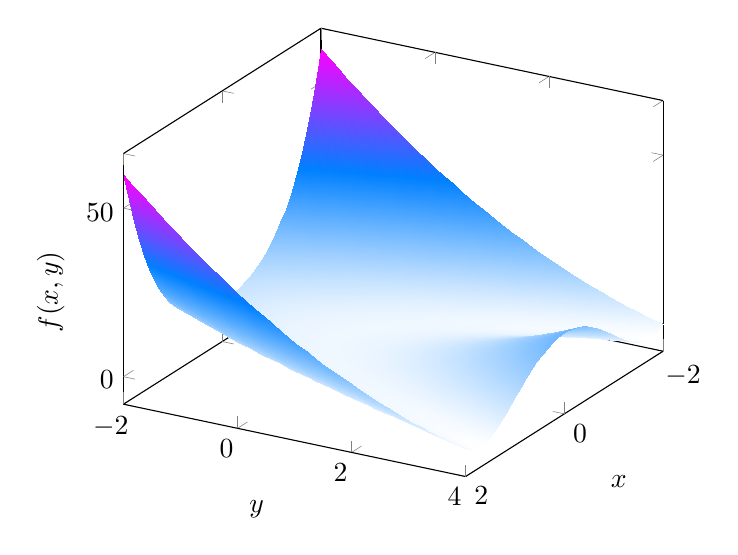
\begin{tikzpicture}
        \begin{axis}[
                view={120}{30},
                  xlabel={$x$},
                     ylabel={$y$},
            zlabel={$f(x,y)$},
                                domain=-2:2,
                                    y domain=-2:4,
                                        samples=40,
                                            samples y=40,
                                                colormap/cool,
                          ]
                \addplot3[
                        surf,
                        shader=interp,
                         ]
                         {(y - x^2)*(y - 2*x^2)};
         \end{axis}
         \end{tikzpicture}
    
\end{parag}

\begin{parag}{Théorème à connaître (condition équivalents sur Hess $f\left(a\right)$, cas $n = 2$}
    \begin{theoreme}
    La proposition suivante s'applique à tous les matrice symmétrique, donc on notre $H := \text{Hess} f\left(a\right) = \begin{pmatrix}r & s \\ s & t \end{pmatrix}$
    \begin{itzemize}
    \item $\lambda_1 > 0, \lambda_2 > 0 \iff \det H > 0$ et $r > 0$
    \item $\lambda_1 <0 , \lambda_2 < 0 \iff  \det H > 0$ et $r < 0$
    \item sgn $\left(\lambda_1\right) \neq $ sgn $\left(\lambda_2\right) \neq 0 \iff \det H < 0$
    \end{itzemize}
    
    \end{theoreme}
    
\end{parag}
\begin{parag}{Démonstration}
    Le déterminant et la trice de $H$ sont invariants par conjugaison. La diagonalisation $H = ODO^T$ donne alors:
    \begin{equation*} rt - s^2 = \det H = \det D = \lambda_1 \lambda_2 \end{equation*}
    \begin{equation*} r + t = Tr\,H = Tr\,D = \lambda_1 + \lambda_2 \end{equation*}
    \begin{subparag}{1 $\implies$}
        Supposons que $\lambda_1 > 0, \lambda_2 > 0$ immédiatement, on a que $\det H = \lambda_1\lambda_2 > 0$.\\
        Ensuite, $\lambda_1\lambda_2 = rt - s^2 > 0$ dont $rt > s^2 \geq 0 \implies$ $r$ et $t$ qui sont de même signe.\\
        De plus, $Tr\,H = \lambda_1 + \lambda_2 = r + t > 0$. On conclut que $r$ doit être strictement positif. (si la multiplication est positive \important{et} l'addition est positif).
    \end{subparag}
    \begin{subparag}{Dans l'autre sens}
        Suppsons que $\det H > 0$ et $r > 0$.\\
        Alors $\det H = \lambda_1\lambda_2 > 0 \implies \lambda_1$ et $\lambda_2$ sont de même signe.\\
        Ensuite, $\lambda_1 \lambda_2 = rt - s^2 > 0$ dont $rt > s^2 \geq 0$ mais $r > 0$ dont $t > 0$ aussi, $Tr\, H \implies r + t = \lambda_1 + \lambda_2 > 0$ et donc on utilise le même arguement que précédemment, $\lambda_1 > 0$ et $\lambda_2 > 0$.
    \end{subparag}
    \begin{subparag}{2}
        Le point 2 est laissé en exercice
        
    \end{subparag}
    \begin{subparag}{3}
        $\det H < 0 \iff \lambda_1\lambda_2 < 0 \iff \lambda_1$ et $\lambda_2$sont de signe opposés.
    \end{subparag}
    
\end{parag}

\begin{parag}{Critère de Sylvester}
    \begin{theoreme}
    Condition équivalentes aux condition suffisantes dans le cas $n = 3$.\\
    Soit $f \in C^2\left(E\right)$ au voisiange de $a$ tel que $\nabla f\left(a\right) = 0$.:\\
    Soit 
    \begin{itemize}
        \item $\Delta_1 = \det Hess_x f\left(a\right)$
        \item $\Delta_2 = \det Hess_{x, y}f\left(a\right)$
        \item $\Delta_3 = \det Hess_{x, y, z} f\left(a\right)$
        
    \end{itemize}
    Alors:
    \begin{itemize}
        \item $\Delta_1 > 0, \Delta_2, \Delta_3 > 0 \iff \lambda_1 > 0, \lambda_2 > 0, \lambda_3 > 0 \iff a$  est un minium local de $f$
        \item $\Delta_1 <0, \Delta_2 < 0 \delta_3 < 0 \iff \lambda_1 < 0 , \lambda_2 <0, \lambda_3 < 0 \iff a$ est un maximum local de $f$
           \item Autrement $\Delta_3 \neq 0 \implies \exists \lambda_i > 0$ et $\lambda_j > 0$ et $\lambda_j < 0 \implies a$ est un point selle de $f$
    \end{itemize}
    \end{theoreme}
\end{parag}
\begin{parag}{Exercice}
    Le  but est de trouver les points critique et de déterminer leur nature.\\
    Soit $f\left(x, y\right) = y^3 + 3y^2 - 4xy + x^2$. Alors $f \in C^{\infty}\left(\mathbb{R}^2\right)$ donc tout les points critiques trouvés sont stationnaire.\\
    On calcule
    \begin{equation*} \nablaf\left(x, y\right) = \left(-4y + 2x, 3y^2 + 6y - 4x\right) \end{equation*}
    Et Pour la Hessienne:
    \begin{equation*} \text{Hess} f\left(x, y\right) = \begin{pmatrix} 2 & -4 \\ -4 & 6y + 6 \end{pmatrix} \end{equation*}
    \begin{equation*} \nabla f\left(x, y\right) = 0 \iff \begin{cases} 2x = 4y \\ 3y^2 + 6y = 4x \end{cases} \iff \begin{cases} x = 2y \\ y\left(3y - 2\right) = 0\end{cases} \end{equation*} 
    Donc si on remplace ce qu'on trouve dans la Hessienne:\\
    On étudie donc les points stationnaire $\left(x, y\right) \in \{\left(0, 0\right), \left( \frac{4}{3},\frac{2}{3}\right)\}$
    Si on cherche donc les points selles:
    \begin{equation*} \text{Hess} f\left(0, 0\right) = \begin{pmatrix}2 & -4 \\ -4 & 6\end{pmatrix} \implies \det = -4 < 0 \end{equation*}
    Ce qui implique que le point $\left(0, 0\right)$ est un point selle.\\
    Si on prends donc Hess $f\left(\frac{4}{3}, \frac{2}{3}\right) = \begin{pmatrix} 2 & -4 \\ -4 & 10\end{pmatrix} = 4 > 0 \implies$ que ce point est un minimum local.
   

\end{parag}



       
       




\lecture{19}{2025-04-28}{Test blanc}{}
\subsection{Corrigé du test blanc}
Ici ce n'est pas le corrigé de la professeur mais moi directement lorsque je fais mes exercices donc il se peut que l'approche ne soit pas rigoureuse peut être même éronnée en quelque sorte:
\begin{parag}{Question 1}
   La solution $y\left(x\right)$ de l'équation différentielle:
   \begin{align*} y'\left(x\right) = \frac{x}{x^2 + 9}\left(y\left(x\right) - 1\right) \end{align*}
   qui satisfait la condition initiale $y\left(0\right) = 7$ vérifie aussi pour $y\left(4\right) = \ldots$.\\
   \begin{subparag}{Corrigé}
       Donc on voit ici en premier lieu que l'équation est une EDVS, on arrive à séparer les $y$ des $x$:
       \begin{align*} y'\left(x\right) = \frac{x}{x^2 + 9}\left(y - 1\right) \\
       \frac{y'}{y - 1} = \frac{x}{x^2 + 9}
    \end{align*}
       A partir de là, il faut alors intégrer des deux côtés et on trouvera la solution:
       \begin{align*} 
            \int \frac{1}{y - 1} dy = \int \frac{x}{x^2 + 0} dx\\
           \ln \left|y - 1\right| + C' = \frac{1}{2}\ln \overbrace{\left|x^2 + 9\right|}^{\geq 0} + C\\
       \left|y - 1 \right| =  \ln C\overbrace{\sqrt{x^2 + 9}}^{\geq 0} \\
       y - 1 = C\sqrt{x^2 + 9}\\
       y = 1 + C \sqrt{x^2 + 9}
   \end{align*}
   Ensuite on va donc trouver la valeur pour $y\left(0\right)$:\\
   On évalue $y\left(0\right) = 1 + C \cdot \sqrt{9} = 1 + 3C \implies C = 2$. Et donc On évalue notre fonction en $y\left(4\right) = 1 + 2\sqrt{16 + 9} = 11$
   \end{subparag}

    
\end{parag}

\begin{parag}{Question 2}
    La solution $y\left(x\right)$ de l'équation différentielle:
    \begin{align*} y' + \frac{1}{x}y = \frac{2}{\left(1 + x^2\right)^2} \end{align*}
    sur l'intervalle $] 0, + \infty [$ qui satisfait la condition initiale $y\left(1\right) = 0$...\\
    Pour cette question soit on apprends par coeur la formule soit on la construit.\\
    On a une équation du type $y' + p\left(x\right)y = f\left(x\right)$. On sait que la solution générale est donné par:
    \begin{align*} y\left(x\right) = y_{hom}\left(x\right) + y_{part}\left(x\right) \end{align*}
    Commençons par la solution homogène:
    \begin{align*} y' + \frac{y}{x} = 0 \end{align*}
    On arrive assez aisément à la séparer:
    \begin{align*} y' &= -\frac{y}{x}\\
    \frac{y'}{y} &= -\frac{1}{x}\end{align*}
    Ensuite on intègre des deux côtés:
    \begin{align*} \int \frac{1}{y} dy = - \int \frac{1}{x}\\
        \ln \left|y\right| = - \ln \left|x\right| + C''
    \end{align*}
    Et à partir d'ici (je vais le faire très proprement un peu overkill)
    \begin{align*} e^{\ln \left|y\right|} = e^{ \ln \left|\frac{1}{x}\right| + C''}\\
        y = e^{C''}e^{\ln \left|\frac{1}{x}\right|}\\
        y = C'''\frac{1}{x}
    \end{align*}
    Après avoir trouver la solution homogène associé $y_{hom} = C\frac{1}{x}$, On utilise la méthode de la variation de la constante pour trouver la solution particulière:
\begin{align*} y_{part}\left(x\right) = c\left(x\right)y_{hom}\left(x\right) \end{align*}
Et par le cours (section \ref{subsec:variationconstante}) on cherchera donc la fonction $c\left(x\right)$:
\begin{align*}c\left(x\right) = \int f\left(x\right) e^{P\left(x\right)}  \end{align*}
On voit ici qu'il faudra faire attention au signe qu'on avait enlevé dans le $\ln$.
Donc on avait trouver pour $P\left(x\right) = \ln \left|Cx\right| $ (on peut mettre le C dedans si on fait une manip avec l'exponentielle).
        \begin{align*} c\left(x\right) &= \int \frac{2x}{\left(1 + x^2\right)^2} dx
        \end{align*}
        Ici j'ai essayé avec les éléments simples mais j'ai rien trouvé donc je vais essayé avec un changement de variable:\\
        Soit $u = 1 + x^2$, on prends $\frac{du}{dx} = 2x$ si on remplace:
            \begin{align*} c\left(x\right) &= \int \frac{2x}{u^2}\frac{du}{2x}\\
            &= \int \frac{1}{u^2}du\\
            &= -\frac{1}{u} + C = -\frac{1}{\left(1 + x^2\right)}
        \end{align*}
        On obtient donc pour la solution particulière:

        \begin{align*} y_{part}\left(x\right) = -\frac{1}{1+x^2}\cdot \frac{1}{x} \end{align*}
On a donc la solution générale:
\begin{align*} y\left(x\right) = \frac{1}{x\left(1+x^2\right)} + \frac{C}{x} \end{align*}
avec $C = \frac{1}{2}$ 

\end{parag}
\begin{parag}{Question 3}
    La solution de $y\left(x\right)$:
    \begin{align*} y'' - y' - 6y = 4e^{-x}
    \end{align*}
    On trouve d'abord la solution homogène:
    \begin{align*} \lambda^2 - \lambda - 6 = 0 \end{align*}
    Qui a pour racine $3$ et $-2$:
    \begin{align*} y_{hom} = C_1e^{3x} + C_2e^{-2x} \end{align*}
    Pour la solution particulière, on pose $y = Ae^{-x}$ avec:\\
    \begin{align*} y' = -Ae^{-x}\;\;\; y'' = Ae^{-x} \end{align*} 
    Si on rempli l'équation on obtient:
    \begin{align*} Ae^{-x} + Ae^{-x} -6Ae^{-x} = 4e^{-x}\\
    2A - 6A = 4\\
    A = -1
\end{align*}
Et donc on trouve que:
\begin{align*} y\left(x\right) = -e^{-x} + C_1e^{3x} + C_2e^{-2x} \end{align*}
Et donc on posera pour les deux conditions tel que:
\begin{align*} 
    \begin{cases}
        -2 = -1 + C_1 + C_2\\
        3 = 1 + 3C_1 - 2C_2
    \end{cases}
   \\
   \begin{cases}
       C_1 = 0\\
       C_2 = -1
   \end{cases}
\end{align*}
Ce qui donne comme sollution final:
\begin{align*} y\left(x\right) = -e^{-x} - e^{-2x} \end{align*}
\end{parag}



\begin{parag}{Question 4}
    Le sous ensemble:
    \begin{align*} E = \{ \left(x, y\right) \in \mathbb{R}^2: x > 1 \text{ et } -1 < xy < 1\} \subset \mathbb{R}^2 \end{align*}
    Est 
    \begin{itemize}
        \item ouvert et borné
        \item fermé et non borné
        \item fermé et borné
        \item ouvert et non borné
    \end{itemize}
    Ici déja on peut voir en quelque sorte a l'oeil nu si le sous-ensemble est ouvert ou fermé. Si l'on le regard comme un ensemble dans $\mathbb{R}$ on voit que tout les $<$ ou $>$ donne des ensemble ouvert (de ce type ] [) ce qui est ``l'équivalent'' de ouvert. et donc peut deviner ici que l'ensemble est ouvert et non fermé.\\
    Pour ce qui est de borné, prenons la deuxième condition, pour montrer qu'un ensemble n'est pas borné il faut montrer qu'il y a une de ces variables qui peut s'étendre jusqu'à l'infini (c'est une sorte d'esquisse de preuve mais ca permet de se répérer lors de qcm).\\
    Donc on prend la deuxième condition: $-1 < xy < 1$ si on prends par exemple: $y = \frac{1}{k + 1}$ et $x = k$ et que nous faisons la limite du produit:
    \begin{align*} \lim_{k \to \infty} \frac{k}{k+1} \end{align*}
    On voit que cette limite est bornée par $1$: soit $k \in \mathbb{R}$prenons:
    \begin{align*} 0 < 1\\
k < k + 1\\
\frac{k}{k+1} < 1
    \end{align*}

    On voit ici donc que $x$ peut tendre vers l'infini et fera toujours parti de l'ensemble, donc l'ensemble n'est pas bornée.

    
    
\end{parag}
\begin{parag}{Question 5}
    Soit $\{\overline{x}_n\}$ la suite d'éléments de $\mathbb{R}^2$ définie par
    \begin{align*} \overline{x_n} = \left(n\sin\left(\frac{\left(-1\right)^n}{n}\right), \frac{\left(-1\right)^n}{n}\sin\left(n\right)\right)^T \end{align*}
    Et on demande la convergence de la suite et/ou elle est bornée.\\
    Pour rappel lorsqu'on traite de suite dans $\mathbb{R}^n$ c'est comme si on traite de suite individuelle donc prenons la première:
    On reconnaît ici bien le schéma de la suite:
    \begin{align*} \lim_{x \to 0} \frac{\sin\left(x\right)}{x} = 1 \end{align*}
    Si on prends la premiere suite on voit que cela ressemble dangereusement comme ceci:
    \begin{align*} \frac{\sin\left(\frac{\left(-1\right)^n}{n}\right)}{\frac{1}{n}} \end{align*}
    Néanmoins à cause du $\left(-1\right)^n$ la suite converge \important{absolument} vers 1 mais oscille entre -1 et 1, donc la suite est bornée mais pas convergente.\\
    Pour l'autre On peut aussi utilise le même arguement mais dans ``l'autre sens'' car on a $\frac{\left(-1\right)^n}{n}$ qui tends vers 0 mais $\sin\left(n\right)$ quant a lui va juste oscillé à l'infini, donc la suite ne pourra jamais converger vers une valeur.\\
    \begin{align*} \left|\frac{1}{n}\sin\left(n\right)\right| \leq \frac{n}{n} \end{align*}
    Et on arrive pas a montrer que la limite tends vers 0 (le sinus se ``comporte'' comme la variable a l'intérieur lorsque celle ci s'approche de 0).
    Et donc la suite est bornée mais pas convergente


\end{parag}


\begin{parag}{Question 6}
    Soit la fonction $f: \mathbb{R}^2 \to \mathbb{R}$ définie par:
    \begin{align*} 
\begin{cases}
    \frac{x^3y + y^3x}{x^2 + y^2} \; \; \text{ si } \left(x, y\right) \neq \left(0, 0\right)\\
    0  \; \; \text{ si } \left(x, y\right) = \left(0, 0\right)
\end{cases}
    \end{align*}
    Comme je soupçonne grandement que la fonction soit dérivable je vais commencer par ça:\\
 Soit $r\left(\overline{x}\right) = f\left(\overline{x}\right) - f\left(\overline{a}\right) - < \nabla f\left(\overline{a}\right), \overline{x}- \overline{a}>$.\\
 Pour ce qui est du gradient, on peut le faire de tête car il y a une puissance de 3 en haut et une puissance de 2 en bas. donc quand tu feras la limite tu tomberas sur 0 des deux côtés. donc $r\left(\overline{x}\right) =  f\left(\overline{x}\right)$
    
 \begin{align*} \lim_{\left(x, y\right) \to \left(0, 0\right)} f\left(x, y\right) = \lim_{r \to 0} \frac{r^4\cos^3\psi\sin\psi + r^4\sin^3\psi\cos\psi}{r^2}\\
     = \lim_{r \to 0} r^2\left(blabla\right) = 0
\end{align*}
Donc la fonction est dérivable.
\end{parag}
\begin{parag}{Question 7}
    Soit la fonction
    \begin{align*} f\left(x, y\right) = \sin\left(\pi x^2 y\right) \end{align*}
    On demande la dérivée directionnelle $D_{\overline{v}}f\left(1, 1\right)$ en suivent le vecteur $\overline{v} = \left(-\frac{1}{\sqrt{5}}, \frac{2}{\sqrt{5}}\right)^T$\\
    Par la definition:
    \begin{align*} \lim_{h \to 0}\frac{ f\left(\overline{e} + h \overline{v}\right)}{h} \end{align*}
    Ce qui nous donne:
    \begin{align*} \lim_{h \to 0} \frac{\sin\left(\pi\left(1-\frac{h}{\sqrt{5}}\right)^2\left(1 + \frac{2h}{\sqrt{5}}\right)\right)}{h}  \end{align*}

    Ce qui après des simplifications:
    \begin{align*}\lim_{h \to 0} \frac{\sin\left(\pi + \frac{-3h^2}{5} + \frac{2h^3}{5\sqrt{5}}\right)}{h}  \end{align*}
    qui nous donne avec les identités trigonométrique:
    \begin{align*} \lim_{t \to 0} \frac{\cos \pi \sin\left(-\frac{3}{h^2} + \frac{2h^3}{5\sqrt{5}}}{h} = 0 \end{align*}
On sait que c'est $0$ parce qu'il y a une puissance $3$ dans le sinus qui va dépasser la puissance $1$ qui est en bas.
\end{parag}
\begin{parag}{Question 8}
    Donc ici il suffit de trouver la jacobienne de $\overline{f}\left(x, y\right)$:
    On calcule donc directement:
    \begin{align*} \nabla f_1\left(x, y\right) = \left(x, y\right)\\
    \nabla f_2\left(x, y\right) = \left(2x, 2y\right)\end{align*}
    Ce qui donne lorsqu'on met en matrice et qu'on évalue en $\left(1, 1\right)$:
    \begin{align*} J_{\overline{f}\left(1, 1\right)} = \begin{pmatrix} 1 & 1 \\ 2 & 2 \end{pmatrix}  \end{align*}
    Et comme on demande directement le gradient de la fonction composée de matrice qui font $1 \times 2 $ avec $2 \times 2$ on a juste besoin de faire le produit matriciel de nos deux jacobienne:
    \begin{align*} \nabla h\left(1, 1\right) = \begin{pmatrix} 1 & -\frac{1}{4} \end{pmatrix} \times\begin{pmatrix} 1 & 1 \\ 2 & 2 \end{pmatrix} = \begin{pmatrix} \frac{1}{2} & \frac{1}{2} \end{pmatrix}  \end{align*}
    Je note juste ici qu'on a pas eu besoin de faire d'autre calcul car aussi $f\left(1, 1\right) = \left(1, 2\right)$ qui était exactement le point du gradient de $f\left(x, y\right)$.
\end{parag}





\lecture{20}{2025-04-30}{Test blanc ou pas}{}

\begin{parag}{Rappel: Thm. Condition suffisante pour un extremum local d'une fonction}
    \begin{theoreme}
        Soit $f: E \to \mathbb{R}$ une fonction de classe $C^2$, $\overline{a} \in E: \; \nabla f \left( \overline{a}\right) = \overline{o}$.\\
        Alors:
        \begin{enumerate}
            \item Si toutes les valeurs propres de Hess$_f\left(\overline{a}\right)$ sont positives $ \implies$ il y a un minimum locale en $\overline{x}$.
            \item $\lambda_1 < 0 , \lambda_2, < 0 \ldots, \lambda_n < 0$ sont négatives $\implies$ un maximum locale en $\overline{x}$.
            \item $\exists \lambda_i > 0$ et $\exists \lambda_j < 0 \implies$ pas \important{pas d'extremum en} en $\overline{x} = \overline{a}$ (un point selle).
        \end{enumerate}
    \end{theoreme}
    
\end{parag}
\begin{parag}{Proposition cas $n = 2$}
    Les condition du Théorème sur la matrice $Hess_f\left(\overline{a}\right)$ sont équivalentes aux conditions suivantes. Posons  
    \begin{align*} \begin{pmatrix} r & s \\ s & t \end{pmatrix} = Hess_f\left(\overline{a}\right) \end{align*}

\end{parag}
\begin{parag}{Cas $n= 3$}
    Lorsque $n = 3$ on a la matrice de Hessienne qui est donnée par:
    \begin{center}
        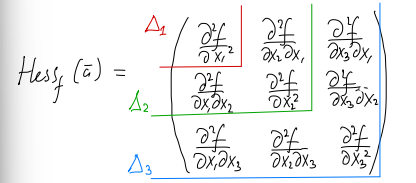
\includegraphics[scale=1.2]{12025-04-30.png}
    \end{center}
\end{parag}


\begin{parag}{Min et Max d'une fonction conitnue sur un ensemble compact}
   \begin{subparag}{Rappel}
       \begin{theoreme}
       Une fonction \important{continue} sur un sous-ensemble \important{compact} $D \subset \mathbb{R}^n$. atteint son min et sont maximum . Formellement:
       \begin{align*} \exists \overline{c_1} \in D: f\left(\overline{c_1}\right) = \text{min}_{\overline{x}\in D}f\left(\overline{x}\right) \\
           \exists \overline{c_2} \in D : f\left(\overline{c_2}\right) = \text{max}_{\overline{x}\in D} f\left(\overline{x}\right)
       \end{align*}
       \end{theoreme}
       
       Pour trouver $\overline{c_1}$ et $\overline{c_2}$ il faut:
       \begin{enumerate}
           \item Trouver les points critiques $\{\overline{c_1}\}$ de $f$ sur $D$ (avec la frontière)
           \item Trouver les points $\{\overline{d_j}\}$ de min, max de $f\left( \nabla D\right)$ calculer les valeurs de $f\left(\overline{d_j}\right)$
           \item Choisir le min et le max de $\{f\left(\overline{c_i}\right), f\left(\overline{d_j}\right)\}$
       \end{enumerate}
   \end{subparag} 
   \begin{subparag}{Exemple}
       $f\left(x, y\right) = 6x^2 + 2x^2y - 3y^2 + 2y + 1$ Trouver le min et le max absolus (global) de $f$ sur le carré $E = \{-2 \leq x, y \leq 2\}$.\\
       La première étape et sur l'ensemble $E = \{-2 < x, y < 2\}$ \\
       On calcule les dérivée partielles:
       \begin{align*} \frac{\partial f}{\partial x} = -12x + 4xy = 4x\left(3-y\right) = 0 \end{align*}
       Qui arrive lorsque $x = 0$ ou $y = 3$ qui n'est pas dans notre ensemble, et donc: $-6y + 2 = 0 \implies y = \frac{1}{3}$, $\left(0, \frac{1}{3}\right) \in E$ .\\
       De l'autre côté:
       \begin{align*} \frac{\partial f}{\partial y} = 2x^2 - 6y + 2 \end{align*}
       En calculant les dérivée partielle seconde:
       \begin{align*} \frac{\partial^2 f }{\partial x^2} = -12 + 4y\\
       \frac{\partial^2 f}{\partial y^2} = -6\\
        \frac{\partial^2 f}{\partial x \partial y} = 4x 
   \end{align*}
   Ce qui implique lorsqu'on calcule la Hessienne:
   \begin{align*} Hess_f\left(0, \frac{1}{3}\right) = \begin{pmatrix} -12 + \frac{4}{3} & 0 \\ 0 & -6 \end{pmatrix} \left(0, \frac{1}{3}\right) \end{align*}
   Et on voit que le déterminant de cette matrice est plus grande que $0$ et que tout les valeurs propres sont négative ($\det > 0$ et $\lambda_i < 0$ nous donne que tout les valeurs propres sont négative (les deux seulement). Ce qui nous donne un maximum locale sur $E$ avec la frontière en $\left(0, \frac{1}{3}\right)$.
       
   \end{subparag}
   \begin{subparag}{Min et Max de $f$ sur la frontière de E}
       Maintenant on cherche le miniment et maximum sur la frontière directement tel que:
       \begin{align*} f\left(x, y\right)_{x = \pm 2} = -24 + 8y - 3y^2 + 2y + 1 \\
       = -3y'2 + 10 y - 23 = g\left(y\right)\end{align*}
       \begin{align*} g'\left(y\right) = -6y + 10 \implies y \frac{5}{3} \end{align*}
       Ce qui nous donne comme élément de l'ensemble $\left(\pm 2, \frac{5}{3}\right)$.\\
       Du côté du $y$:
       \begin{align*} f\left(x, y\right)_{y = 2} = -6x^2 + 4x^2 -12 + 4 + 1 = -2x^2 - 7 = h_1\left(x\right) \implies \left(0, 2\right) \text{ est un max local} \end{align*}
       Avec $h_1'\left(x\right) = -4x, h_1''\left(x\right) = -4 < 0$.\\
       \begin{align*} f\left(x, y\right)_{y = -2} = -6x^2 - 4x^2 -12 -4 + 1 = -10x^2 - 15 = h_2\left(x\right) \implies \left(0, -2\right) \text{ este un max local} \end{align*}
       Avec $h_2'\left(x\right) = -20x$ et $h_2''\left(x\right) = -20 < 0$.\\
       On regarde finalement les coins:
        \begin{align*} f\left(\pm 2, 2\right) = -15\\
        f\left(\pm 2, -2 \right) = -55\end{align*}
        On cherche donc sur toute les valeurs qu'on a trouvées le min et le max qui nous donne $\frac{4}{3}$ pour le max global sur $E$ et $-55$ le minimum global sur $E$. avec:
        \begin{align*} f\left(0, \frac{1}{3}\right) = \frac{4}{3}\\
        f\left(\pm 2, -2\right) = -55 \end{align*}

       
   \end{subparag}
\end{parag}


\subsection{Théorème des fonctions implicites}
\begin{parag}{Question}
    Fonction implicite: Une dépendance $f = f\left(\overline{x}\right)$ qui est définie par une équation.\\
   La question posée est, est ce que l'équation $F\left(x, y\right) = 0$ définit une fonction $y = y\left(x\right)$? 
   \begin{subparag}{Exemple 1}
        Soit $F\left(x, y\right) = x + 3y = 0$\\
        On voit ici que a fonction $y = f\left(x\right)$ et donnée par: $y = - \frac{1}{3}x$ et on voit que cela est définit partout.
   \end{subparag}
   \begin{subparag}{Exemple 2}
       Soit la fonction $F\left(x, y\right) = x^2 + y^2 - 1 = 0$. Et soit $\left(a, b\right) \in$ le cercle, alors $a^2 + b^2 + 1 = $
       Si $b > 0 \implies y = \sqrt{1 - x^2}$ au voisinage de $\left(a, b\right)b > 0$\\
       Si $b < 0 0> y = -\sqrt{1-x^2}$ au voisinage de $\left(a, b\right)$:  $b < 0$.
       Si $b = 0$ on a deux solution pour chaque $x$ dans le voisinage $\left(\pm 1, 0\right)$
   \end{subparag}
    
\end{parag}


\begin{parag}{Surface}
    \begin{definition}
        Une surface (\important{ligne}) de niveau d'une fonction $F\left(x, y, z\right)$ ou ($F\left(x, y\right)$) est la surface (ligne) définie par l'équation
        \begin{align*} F\left(x, y, z\right) = C , \; \; C \in \mathbb{R}\end{align*}

    \end{definition}
    
    \begin{subparag}{Exemple 3}
        soit la fonction $F\left(x, y\right) = 2-ye^x + xe^y$ on cherche $y = f\left(x\right)$ autour d'une point donné $\left(0, 1\right)$?\\
        \begin{center}
            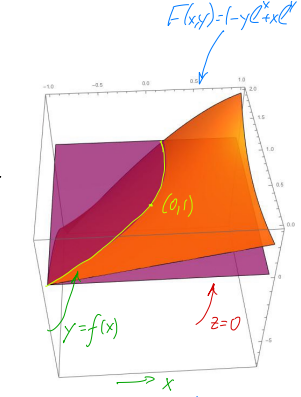
\includegraphics[scale=0.8]{22025-04-30.png}
        \end{center}
        Soit $\left(x, y\right) = \left(0, 1\right)$. On vérifie que $F\left(x, y\right) = 0$ définit autour de $\left(0, 1\right)$ une fonction $y = f\left(x\right)$ telle que $F\left(x, f\left(x\right)\right)= 0$ au voisinage de $x = 0$ et trouver  $f'\left(0\right)$.\\
        On trouve d'abord:
        \begin{align*} \frac{\partial F}{\partial y}= -e^x xe^y \text{ en (0, 1) } = -1 \neq 0 \end{align*}
        Ce qui implique que le TFI est appliquable.\\
        Il existe alors une fonction $f\left(x\right)$ tel que $y = f\left(x\right)$au voisinage de $\left(0, 1\right)$: $F\left(x, f\left(x\right)\right) = 0$. et
        \begin{align*} f'\left(x\right) = -\frac{\frac{\partial F}{\partial x}\left(x, y\right)}{\frac{\partial F}{\partial y}\left(x, y\right)} =- \frac{ye^x + e^y}{-e^x + xe^y}_{\left(0, 1\right)} = -\frac{-1 + e}{-1} = -1 + e = f'\left(0\right) \end{align*}
        On a donc pour l'equation de la tangente au point $\left(0, 1\right)$ à la courbe $y = f\left(x\right)$.
        \begin{align*} y - 1 = \left(-1 + e\right)\left(x - 0\right)\\
        y = 1 + \left(e-1\right)x\end{align*}
        
        
    \end{subparag}
\end{parag}
\begin{parag}{Théorème des fonctions implicites}
    \begin{theoreme}
    $F: E \to \mathbb{R}$ une fonction de classe $C^1$ au voisinage de $\overline{a} = \left(a_1, \ldots, a_n\right) \in E$ telle que:
   \begin{align*} 
       F\left(\overline{a}\right) &= 0\\
       \frac{\partial F}{\partial x_n}\left(\overline{a}\right) &\neq 0
   \end{align*}
   Alors il existe un voisinage $B\left( \overline{a}', \delta\right)$ de $\overline{a}' = \left(a_1, a_2, \ldots, a_{n-1}\right)\in \mathbb{R}^{n-1}$ et une fonction $f : B\left(\overline{a}', \delta\right) \to \mathbb{R}$ telle que\\
   \begin{enumerate}
       \item $a_n = f\left(a_1, \ldots a_{n-1}\right)$
       \item $F\left(x_1, x_2, \ldots, x_{n-1}, f\left(x_1, \ldots, x_{n-1}\right)\right) = 0 $ et cela $\forall \left(x_1, x_2, \ldots, x_{n-1}\right) \in B\left( \overline{a}', \delta\right)$.
   \end{enumerate}
   
    \end{theoreme}
    De plus, $f$ est de classe $C^1$ dans un voisinage de $\overline{a}'$ et on a
    \begin{align*} \frac{\partial f}{\partial d_p} \left(x_1, x_2, \ldots, x_{n-1}\right) = - \frac{\frac{\partial F}{\partial x_p}\left(x_1, \ldots, x_{n-1}, f\left(x_1, \ldots, x_{n-1}\right)\right)}{\frac{\partial F}{\partial x_n}\left(x_1, \ldots, x_{n-1}, f\left(x_1, \ldots, x_{n-1}\right)\right)} \; \; \forall p \in \{1, \ldots, n-1\} \end{align*}

\end{parag}
\begin{parag}{Cas particulier du TFI: deux variables}
    Soit $F\left(x, y\right): E \to \mathbb{R}$ de classe $C^1$ telle que $F\left(a,b\right) = 0$ et $\frac{\partial F}{\partial y}\left(a, b\right) \neq 0$.\\
    Alors l'équation $F\left(x, y\right) = 0$ définit localement autour de $\left(a, b\right)$ une fonction $y = f\left(x\right) $ telle que:
    \begin{enumerate}
        \item $f\left(a\right) = b$
        \item $F\left(x_1, f\left(x\right)\right) = 0$
        \item $f'\left(x\right) = - \frac{\frac{\partial F}{\partial x}\left(x, f\left(x\right)\right)}{\frac{\partial F}{\partial y}\left(x, f\left(x\right)\right)}$
    \end{enumerate}
    Cela veut dire que l'on peut calculer $f'\left(a\right)$ sans savoir la formule explicite pour $f\left(x\right)$.
    
\end{parag}

\begin{parag}{Cas particulier du TFI: trois variables}
    Soit $F\left(x, y, z\right): E \to \mathbb{R}$ de classe $C^{1}$ tel que $F\left(a,b, c\right) = 0$ et $\frac{\partial F}{\partial z}\left(a, b, c\right) \neq 0$.\\
    Alors il existe localement une fonction $z = f\left(x, y\right)$ telle que 
    \begin{enumerate}
        \item $f\left(a, b\right) = c$
        \item $F\left(x, y, f\left(x, y\right)\right) = 0$ pour tout couple, $\left(x, y\right)$ dans un voisinage de $\left(a, b\right)$
        \item $\frac{\partial f}{\partial x}\left(x, y\right) = - \frac{\frac{\partial F}{\partial x}\left(x, y, f\left(x, y\right)\right)}{\frac{\partial F}{\partial z}\left(x, y, f\left(x, y\right)\right)}$; $\partial $ je ferais après
        
    \end{enumerate}
    
    
\end{parag}

\begin{parag}{Q16}
    L'équation $F\left(x, y\right) = \sin\left(x + y\right)\cos\left(x-y\right) - \frac{1}{2} = 0$. On cherche $g\left(x\right)$.\\
\begin{align*} \frac{\partial F}{\partial x}\left(x, y\right) = \cos\left(x + y\right)\cos\left(x-y\right) - \sin\left(x + y\right)\sin\left(x-y\right) \end{align*}
\begin{align*} \frac{\partial F}{\partial y}\left(x, y\right) = \cos\left(x + y\right)\cos\left(x-y\right) + \sin\left(x+y\right)\sin\left(x-y\right) \end{align*}

Donc si on simplifie:
\begin{align*} \frac{\cos\left(2x\right)}{\cos\left(2y\right)} \end{align*}
    On pose les questions: $\exists x =  h\left(y\right)$ et $\exists y =  g\left(x\right)$ et nous voyons que cela est vrai seulement pour $x = h\left(y\right)$.:\\
Comme dit précédemment on trouve donc la dérivée de la fonction grâce a notre formule:
\begin{align*} h'\left(y\right) = - \frac{\frac{\partial F}{\partial y}}{\frac{\partial F}{\partial x}}_{\left(\frac{\pi}{2}, \frac{\pi}{4}\right)} = -\frac{0}{-1}\end{align*}
On obtient logiquement pour la pente de la tangent $x =  h\left(y\right)$ en $\left(\frac{\pi}{2}, \frac{\pi}{4}\right)$ est $0$.

\end{parag}




\lecture{21}{2025-05-05}{TFI}{}
\begin{parag}{Rappel TFI}
    \begin{subparag}{TFI en $2$ variables}
        \begin{theoreme}
            Soit $F\left(x, y\right) : E^{\subset \mathbb{R}^2} \to \mathbb{R}$ de classe $C^1$ telle que $F\left(a, b\right) = 0$ et $\frac{\partial F}{\partial y}\right)a, b\right) \neq 0 $ Alors l'équation $F\left(x, y\right) = 0$ définit localement autour de $\left(a, b\right)$ une fonction $y =  f\left(x\right)$ telle que:
            \begin{itemize}
                \item $f\left(a\right) = b$
                \item $F\left(x, f\left(x\right)\right) = 0$pour tout $x$ dans un voisinage de $x = a$
                \item $f'\left(x\right) = - \frac{\frac{\partial F}{\partial x}\left(x, y\right)}{\frac{\partial F}{\partial y}\left(x, y\right)}_{\left(x, f\left(x\right)\right)}$
            \end{itemize}
        \end{theoreme}
    \end{subparag}
    
    \begin{subparag}{TFI en 3 variables}
        Soit $F\left(x, y, z\right): E \to \mathbb{R}$ de classe $C^1$, tel que $F\left(a, b, c\right) = 0$ et $\frac{\partial F}{\partial z}\left(a, b, c\right) \neq 0$.\\
       Alors il existe localement une fonction $z =  f\left(x, y\right)$ telle que:
       
       \begin{enumerate}
           \item j'ai pas eu le temps parce que vim compuile pas
       \end{enumerate}
       
    \end{subparag}
\end{parag}
\begin{parag}{Exemple 4}
    Soit $F\left(x, y, z\right) = x\cos y + y \cos z + z \cos x -1$\\
    En premier lieu on vérifie les conditions, $F\left(0, 0, 1\right) = 0$ et que $F\left(x, y, z\right) = 0$ definit autour de $\left(0, 0, 1\right)$ une fonction $z = f\left(x, y\right)$ telle que $F\left(x, y, f\left(x, y\right)\right) = 0$. On cherche ensuite $\frac{\partial f}{\partial x} \left(0, 0\right)$ et $\frac{\partial f}{\partial y} \left(0, 0\right)$\\
   \begin{enumerate}
       \item $F\left(0, 0, 1\right) = 0 \cos 0 + 0 \cos 1 + 1 \cos 0  1 = 1  1 = 0$
       \item $\frac{\partial F}{\partial z}\left(0, 0, 1\right) = -y\sin z + \cos x$ en $\left(0, 0, 1\right)$ ce qui implique:
           \begin{align*} -0 \sin 1  + \cos 0 =  1 \neq 0 \implies \text{ TFI est applicable} \end{align*}
           Ce qui implique que $\exists z = f\left(x, y\right)$ la solution de $F\left(x, y, z\right) = 0$ autout de $\left(0, 0, 1\right)$
       \item 
       \begin{align*} \frac{\partial f}{\partial x} \left(0, 0\right) = - \frac{\frac{\partial F}{\partial x}\left(x, y, z\right)}{\frac{\partial F}{\partial z}\left(x, y, z\right)} = - \frac{\cos y - z \sin x}{- y\sin z + \cos x} =  -\frac{1}{1} = -1 \end{align*}
   \item 
   \begin{align*} \frac{\partial f}{\partial y}\left(0, 0\right) =  - \frac{\frac{\partial F}{\partial y}\left(x, y, z\right)}{\frac{\partial F}{\partial z}\left(x, y, z\right)} = - \frac{-x\sin y + \cos z}{-y \sin z + \cos x} = -\cos 1 = -\cos 1\end{align*}
   \end{enumerate}
   Donc ici lorsqu'on a une question de ce type lors de l'examen on voit que ces une question  qui est censée être facile vu que sa résolution est très algorithmique.
\end{parag}
\begin{parag}{Plan tangent}
   Des lors grâce à ce qu'on a trouvé et aussi comme on à trouvé que l'équation du plan tangent est:
   \begin{align*} z = f\left(a, b\right) + <\nabla f\left(a, b\right), \left(x - a, y -b\right)> \end{align*}
   Comme on a déjà trouvé les dérivée partielles grâce à notre petit exemple on a:
   \begin{align*} z = 1 + <\left(-1, -\cos 1\right), \left(x-0, y-0\right) > = 1 + \left(-x\right) + \left(-\cos 1\right) \cdot y = 1 -x - \left(\cos 1\right) \cdot  y\\
    \implies z = 1 - x - \left(\cos 1\right) \cdot  y \text{ est l'équation du plan tangent à la surface}
   \end{align*}
   (Surface qui est celle de $z = f\left(0, 0, 1\right)$


\end{parag}
\subsection{Application de TFI Equation d'un (hyper plan tangent à la surface définie par une équation}

\begin{parag}{Application de TFI:}
        Soit $F\left(x_1, \ldots, x_n\right)$ de classe $C'$ sur $E \subset \mathbb{R}^n$ et $\exists i: i \leq i \leq n$ tel que:
        \begin{align*} p\frac{\partial F}{\partial x_i}\left(\overline{a}\right) \neq 0\text{ pou un } \overline{a} \in E \text{ où } F\left(\overline{a}\right) = 0 \end{align*}
        Alors le TFI implique que l'équation $F\left(x_1, \ldots, x_n\right) = 0$ définit une (hyper) surface $x_i = f\left(x_1, \ldots , x_n \right)$ (où on a enlevé le i)
\end{parag}
\begin{parag}{Equation du plan tangent  }
    Si $\nerline{a}\right) \neq 0$, alors $DF\left(\overline{a}, \overline{v}\right) = 0 \iff \overline{v}$ est tangent à la hyper surface de niveau.
    \begin{align*} DF\left(\overline{a}, \overline{v}\right) = <\nabla F\left(\overline{a}\right), \overline{v}> = 0 \text{ pour tout vecteur } \overline{v}\text{ dans l'hyperplan tangent à } F\left(\overline{x}\right) \end{align*}
    Et tout cela au point $\overline{x} =  \overline{a}$
    Ce qui implique et se fait implique (ssi):
    \begin{align*} \overline{v} =  \left(\overline{x} - \overline{a}\right) \perp \nabla F\left(\overline{a}\right) \end{align*}
    \begin{theoreme}
    L'équation de l'hyperplan tangent à $F\left(\overline{x}\right) = 0$ au point $\overline{a}$ : $F\left(\overline{a}\right) = 0$ est:
        \begin{formule}
            \begin{align*} 
            <F(a, b, c), (x-a, y-b, z-c)> = 0
            \end{align*}
        \end{formule}
        
    \end{theoreme}
\end{parag}







\begin{parag}{Exemple 4}
    soit donc la même fonction $F\left(x, y, z\right) = x\cos y + y \cos z + y \cos z + z \cos x - 1 = 0$ et on a aussi que $\overline{a} = \left(0, 0, 1\right)$\\
\begin{align*} \nabla F\left(0, 0, 1\right) = \left(1, \cos 1, 1\right) \neq \overline{0} \\
\implies <\left(1, \cos 1, 1\right), \left(x-0, y-0, z-1\right)> = 0\\
\implies x + y \cos 1 + z-1 = 0\\
\implies z =  1 - x - \left(\cos 1\right)y
\end{align*}
Ce qui nous donne bien l'équation du plan tangent\\
Ce qui pourrait donner comme exercice: $y =  g\left(x, z\right)$ tel que:
\begin{align*} F\left(x, g\left(x, z\right), z\right) = 0 \text{au voisinnage de } \left(0, 0, 1\right) \end{align*}
\end{parag}
\begin{parag}{Exemple 5}
    Soit l'ellipsoïde $F\left(x, y, z\right) =  x^2 + 2y^2 + 3z^2 - 6 = 0$\\
    Soit $\left(a, b, c\right) \in \mathbb{R}^3$: $a^2 + 2b^2 + 3c^2 = 6 $ Trouver une équation du plan tangent à la surface au point $\left(a, b, c\right)$.\\
    \begin{align*} 
        \nabla F\left(x, y, z\right) = \left(2x, 4y, 6z\right)_{\left(a, b, c\right)} = \left(2a, 4b, 6c\right) \neq \overline{0} \;\; \forall \left(a, b, c\right) \in \text{l'ellipsoide}\\
        <\nabla F\left(a, b, c\right), \left(x-a, y-b, z-x\right) > = 0
    \end{align*}
    Ce qui nous donne l'équation du plan tangent en $\left(a, b, c\right)$:
    \begin{align*}
        <\left(2a, 4b, 6c\right), \left(x-a, y-b, z-c\right)> = 2ax -2a^2 + 4by - 4b^2 + 6cz - 6c^2 = 0 \\ 
    ax + 2by + 3cz - a^2 2b^2 - 3c^2 = 0\\
ax + 2by + 3cz = 6
\end{align*}
    \end{parag}




\begin{parag}{Lien avec le plan tangent au graphique d'une fonction $z = f\left(x, y\right)$}
    
    Si $F\left(x, y, z\right) = z-f\left(x, y\right) \implies \frac{\partial F}{\partial z} = 1 \neq 0 $ Ce qui implique que $\nabla F\left(x, y, z\right) \neq \overline{0}$. Alors:
    \begin{align*} 
    \forall \left(x,y, z\right) \text{ où } z = f\left(x, y\right)\end{align*}
    Si $c = f\left(a, b\right) \iff \left(a, b, c\right) \in $ surface de niveau $F\left(x, y, z\right) = 0$\\
    Et donc par le TFI l'équation du plan tangent au point $\left(a, b, c\right)$ est:
    \begin{align*} \nabla F\left(a, b, c\right), \left(x-a, y-b, z-c\right) > = 0 \end{align*}


    \begin{subparag}{Développement}
        Donc is on développe notre équation:
        \begin{align*} 
            \frac{\partial F}{\partial x} \left(a, b, c\right)\cdot \left(x-a\right) + \frac{\partial F}{\partial y} \left(a, b, c\right) \cdot  \left(y - b\right) + \frac{\partial F}{\partial z} \left(a, b, c\right)\cdot  \left(z-x\right) = 0\\
                - \frac{\partial f}{\partial x} \left(a, b\right) - \frac{\partial f}{\partial y} \left(a, b\right) + z - f\left(a, b\right) = 0\\
                z = f\left(a, b\right) + <\nabla f\left(a, b\right), \left(x-a, y-b\right)>
        \end{align*}
    \end{subparag}
\end{parag}

\begin{parag}{Example: droite tangent à la fonction définie implicitement:}
    \begin{subparag}{Exemple 6}
        Soit la surface tel que: $F\left(x, y\right) = x^{\frac{2}{3}} + y^{\frac{2}{3}} - 4 = 0$ Alors, le but est de trouver l'équation de la tangente au point $\left(a, b\right) = \left(2^{\frac{3}{2}}, 2^{\frac{3}{2}}\right)$

        Donc on met nos valeurs dedans: $2^{\frac{2}{3}}^{\frac{2}{3}} + 2^{\frac{2}{3}}^{\frac{2}{3}} - 4 = 0 $ ce qui implique que $F\left(a, b\right) = 0$\\
On calcule ensuite le gradient:
\begin{align*} \nabla F\left(x, y\right) = \left(\frac{2}{3}x^{-\frac{1}{3}}, \frac{2}{3}y^{-\frac{1}{3}}\right)_{\left(2^{\frac{3}{2}}, 2^{\frac{3}{2}}\right)} = \left(\frac{\sqrt{2}}{3}, \frac{\sqrt{2}}{3}\right) \neq \overline{0} \end{align*}
On a donc que l'équation de la tangente est $< \nabla F\left(a, b\right), \left(x-a, y-b\right)> = 0$\\
On va donc développer et simplifier:
\begin{align*} 
    <\left(\frac{\sqrt{2}}{3},\frac{\sqrt{2}}{3}\right) , \left(x - 2^{\frac{3}{2}}, y - 2^{\frac{3}{2}}\right)> = \frac{\sqrt{2}}{3} \left(x-2^{\frac{3}{2}}\right) + \frac{\sqrt{2}}{3}\left(y - 2^{\frac{3}{2}}\right) =  0\\
        x + y - 2\cdot 2^{\frac{3}{2}} = 0\\
        x + y - 2 ^{\frac{5}{2}} =  0
\end{align*}
    \end{subparag}
    
\end{parag}


\begin{parag}{Question 17}
   Soit la fonction $f\left(x, y\right) = \ln\left(x + y^2\right) - y^2 - x^2$ 
   Alors sur son domaine de définition la fonction $f$ on demande un peu tout ce qui se passe avec les points stationnaires etc..\\
   On commence par calculer le gradient:
   \begin{align*} 
        \nabla f\left(x, y\right) = \frac{1}{x + y^2} - 2x, \frac{2y}{x + y^2}- 2y
   \end{align*}
   On chercher donc comment on peut arriver a trouver les 0 tel que:
   \begin{align*} 
        \nabla f\left(x, y\right) =  \overline{0}\\
        \begin{cases}
            \frac{1}{x + y^2} -2x = 0\\
            \frac{2y}{x+y^2} - 2y = 0
        \end{cases} \implies 1 = 1\frac{1}{x + y^2}
   \end{align*}
   et ce qui si on simplifie grâce a notre premiere équation:
    \begin{align*} 
        2x = \frac{1}{x + y^2} = 1 \implies x = \frac{1}{2}
    \end{align*}
    On obtient donc $y = \pm \sqrt{\frac{1}{2}}$ ce qui nous donne donc 2 points stationnaires, on peut aussi poser $y = 0$ ce qui nous donne bien $0$ pour la dérivée partielle de $y$ et pour celle de $x$:
    \begin{align*} \frac{1}{x + y^2} = 2x\\
        \frac{1}{x} = 2x \implies x^2 = \frac{1}{2}\\
        x = \pm \sqrt{\frac{1}{2}}
    \end{align*}
    et il faut faire attention au domaine de définition qui ne prends par en compte le point $\left(-\sqrt{\frac{1}{2}}, 0\right)$ caril n'est pas définit pour le $\ln$ et donc on obtient $3$ point stationnaire.\\
    On va maintenant calculer la hessienne avec ces quatre valeurs  propres:
\end{parag}



\subsection{Extrema liés. Méthode des multiplicateurs de Lagrange}

\begin{parag}{Théorème cas $n = 2$}
    \begin{theoreme}
    Condition nécessaire pour un extremum sans contrainte.\\
    Soient les fonctions $f, g: E \to \mathbb{R}$ de classe $C^1$.\\
    Supposons que $f\left(x, y\right)$ admet un extremum en $\left(a, b\right) \in E$ sous la contrainte $g\left(x, y\right) = 0$:
    \begin{align*} \text{min}, \text{max}\left\{f\left(x, y\right): \left(x, y\right) \in E \text{ et } g\left(x, y\right) = 0\right\} \end{align*}
    et que $\nabla g\left(x, y\right) \neq \overline{0}$ pour $g\left(x, y\right) = 0$ Alors il existe $\lambda \in \mathbb{R}$ tel que:
    \begin{formule}
        \begin{align*} \nabla f\left(a, b\right) = \lambda \nabla g\left(a, b\right) \end{align*}
    \end{formule}
    
    \end{theoreme}
    
\end{parag}


\begin{parag}{Extrema liés interpretation géométrique}
    Soit $g\left(x, y\right) = 0$ la contrainte $\implies$ c'est une courbe d niveau:
    \begin{align*} \implies \nabla g\left(x, y\right) \perp \text{ a la courbe}, \nabla g\left(x, y\right) \neq 0 \end{align*}
    Si $\left(a, b\right)$ est un extremum local de $f\left(x, y\right)$ sur la courbe. Alors: 
    \begin{align*} Df\left(a, b\right) \left(\overline{v} \text{tangent à } g\left(x, y\right) = 0\right) =  <\nabla f\left(a, b\right), \overline{v}_{tang}> = 0 \end{align*}
    On obtient donc que:
    \begin{align*} \nabla f\left(a, b\right) =  \overline{0} \implies \nabla f\left(a, b\right) = 0 \cdot  \nabla g\left(\overline{a}, b\right) \cdot  \lambda = 0\\
        \nabla f\left(\overline{a}, b\right) \perp \text{ à la courbe} \iff \nabla f\left(a, b\right) = \lambda \nabla g\left(a, b\right), \lambda \neq 0
    \end{align*}
    Ce qui implique finalement:
    \begin{align*} \exists \lambda \in \mathbb{R}: \nabla f\left(a, b\right) = \lambda \cdot  \nabla g\left(a, b\right) \end{align*}
    Qui est le théorème de Lagrange.
    
\end{parag}


\lecture{22}{2025-05-07}{Méthode de Lagrange}{}
\subsubsection{Rappel Extrema liés. Méthode des multiplicateur de Lagrange}

\begin{parag}{Théorème (cas $n = 2$)}
    \begin{theoreme}
        Condition nécessaire pour un extremum sans contrainte.(mais qui n'est pas suffisante)\\
        Soit les fonctions $f, g: E^{\subset \mathbb{R}^2} \to \mathbb{R}$ de classe $C^1$.\\
        Supposons que $f\left(x, y\right)$ admet un extremum en $\left(a, b\right) \in E$ sous la contrainte $g\left(x, y\right) = 0$, Ce qui se dit tel que:
        un extremum de $\left\{f\left(x,y\right): \left(x, y\right) \in E \text{ et } g\left(x, y\right) = 0\right\}$. Et que $\nabla g\left(a, b\right) \neq \overline{0}$. \\
        Alors il existe $\lambda \in \mathbb{R}$ tel que:
        \begin{align*} 
            \nabla f\left(a, b\right) = \lambda \nabla g\left(a, b\right)
        \end{align*}
    \end{theoreme}
    
    \begin{definition}
        $\lambda$ est le multiplicateur de Lagrange
    \end{definition}
\end{parag}
\begin{parag}{Extrema liés: interpretation géométrique}
    soit $g\left(x, y\right) = 0 $ avec la contrainte que c'est sur une courbe de niveau, alors $\nabla g\left(x, y\right) \perp $ à cette courbe de niveau, $\nabla g\left(x, y\right) \neq \overline{0}$ (contrainte mentionnée dans le théorème).\\
    Si $\left(a, b\right)$ est un extremum local de $f\left(x, y\right)$ sur la courbe, il y a deux possibilités:
    \begin{itemize}
        \item Soit c'est un extremum local de $f$ sur $\mathbb{R}^{2}$
        \item Soit ce n'est pas un extremum local de de $f$ sur $\mathbb{R}^{2}$ mais un extremum local seulement sur la courbe.
    \end{itemize}
    Ce qui implique donc dans chaque cas:
    \begin{itemize}
        \item $\nabla f\left(a, b\right) = 0$
        \item $\nabla f\left(a, b\right) \perp$ à la courbe de niveau.
    \end{itemize}
    Ce qui implique donc que:
    \begin{itemize}
        \item $\nabla f\left(a, b\right) = 0 \cdot \nabla g\left(a, b\right)$
        \item $\nabla f\left(a, b\right) =  \lambda \cdot  \nabla g\left(a, b\right)$ où $\lambda \neq 0$
    \end{itemize}
    
\end{parag}

\begin{parag}{Démonstration}
    Pour la démonstration je renvoie le pdf de Joachim Favre qui est plus propre et plus clair que moi \\
Les idées majeurs sont TFI, qui permet de mieux réecrire notre fonction, par la suite la dérivée de la composition (avec la jacobienne avec le ``changement de variable''  :)
\begin{align*} \begin{pmatrix} 1 \\h\left(x\right)  \end{pmatrix}  \end{align*}



\end{parag}

\begin{parag}{Extrema liés cas général}
    \begin{theoreme}
        Soit $f, g_1, \ldots, g_m : E^{ \subset \mathbb{R}^{n}} \to \mathbb{R}$ les fonctions de classe $C^1$ tel que $m \leq n - 1$. Soit $\overline{a} \in E $ un extremum de $f$ sous les contraintes $g_1\left(\overline{x}\right) = \ldots = g_m\left(\overline{x}\right) = 0$.\\
        Supposons que les vecteurs $\nabla g_1\left(\overline{a}\right), \ldots, \nabla g_m\left(\overline{a}\right)$ sont linéairement indépendants.\\
        Alors il existe un vecteur $\overline{\lambda} = \left(\lambda_1, \ldots, \lambda_m\right) \in \mathbb{R}^{m}$ tel que:
        \begin{formule}
            \begin{align*} \nabla f\left(\overline{a}\right) = \sum_{k = 1}^{m} \lambda_k \nabla g_k\left(\overline{a}\right) \end{align*}
        \end{formule}
        
    \end{theoreme}
    Ici on utilise linéairement indépendant comme ``analogie'' à $\nabla g\left(a, b\right) \neq \overline{0}$ lorsque on avait $g: \mathbb{R}^{n} \to \mathbb{R}$. (maintenant on va dans $\mathbb{R}^{n}$)
    En particulier si on cherche un extremum de $f$ sour la contrainte $g\left(\overline{x}\right) = 0$ on obtient les équations:
    \begin{align*} 
        \begin{cases}
            \nabla f\left(\overline{x}\right) =  \nabla g\left(\overline{x}\right)\; \; \; \text{ si } \nabla g\left(\overline{x}\right) \neq 0 \text{ pour } g\left(\overline{x}\right) = 0\\
            g\left(\overline{x}\right) = 0
        \end{cases}
    \end{align*}
\end{parag}
\begin{parag}{Exemple 1}
    Trouver les extrema de la fonction $f\left(x, y, z\right) = 4x + 2y - z$ sous la contrainte $g\left(x, y, z\right) = x^2 + y^2 + z^2 - 21 = 0$ (qui est donc une sphère de rayon $\sqrt{21}$).\\
    On commence avec le théorème, le gradient: $\nabla g\left(2x, 2y, 2z\right) \neq \left(0, 0, 0\right)$ sur la sphère de rayon $\sqrt{21}$\\
    Alors, par le théorème de Lagrange, si on a $\left(x, y, z\right) \in $ sphère qui est un point d'extremum local de $f$ sur la sphère, alors, $\exists \lambda \in \mathbb{R}$ tel que:
    \begin{align*} 
        \nabla f\left(x, y, z\right) = \lambda \nabla g\left(x, y, z\right)\\
        x^2 + y^2 + z'2 =  21
    \end{align*}
    On a donc ici quatre équation dont les trois du gradients:
    \begin{align*}
        \begin{case}
            \left(4, 2, -1\right) =  \lambda \left(2x, 2y, 2z\right)\\
            x^2 + y^2 + z^2 =  21
        \end{case}
    \end{align*}
    Donc si on pose notre première trois relations:
    \begin{align*}
        \begin{case}
            4 =  \lambda 2x\\
            2 =  \lambda 2y \\
            -1 =  \lambda 2z
            \end{case} \implies \begin{case}
            x =  \frac{2}{\lambda}\\
            y =  \frac{1}{\lambda}\\
            z =  - \frac{1}{2\lambda}
        \end{case}
        \implies \begin{case} x =  -4z \\ y =  -2z \end{case}
    \end{align*}
    Et cela dans $g\left(x, y, z\right) =  0$.\\
    On implique ce qu'on trouve à notre contrainte:
    \begin{align*} 16z^2 + 4z^2 + z^2 =  21 \implies 21z^2 =  21 \implies z = \pm 1 \end{align*}
    Ce qui nous implique que: $z =  -1, y = 2, x = 4$ ou alors l'opposé qui nous donne:
    \begin{align*} \left(-4, -2, 1\right), \; \; \left(4, 2, -1\right) \end{align*}
    On remet notre valeur dans notre fonction:
    \begin{align*} f\left(-4, -2, 1\right) =  4x + 2y - z =  -16 -4 -1 =  -21\\
                    f\left(4, 2, -1\right) =  16 + 4 + 1 =  21
    \end{align*}
    Néanmoins ici on parle d'une sphère qui est un espace fermé dans $\mathbb{R}^{3}$, qui est aussi borné. Comme on est donc dans un ensemble compact, et puisque que notre fonction est aussi continue sur cette ensemble alors, notre fonction atteint \important{forcement} son maximum et son minimum sur la sphère.\\
    Ce qui implique que $f$ atteint son minimum et son maximum absolus sur la sphère.\\
    On va donc chercher les plans où il y a le minimum et le maximum, logiquement ces plans se retrouvent au sommets de la sphère, ces plans sont donc tangent à cette sphères:
    \begin{center}
        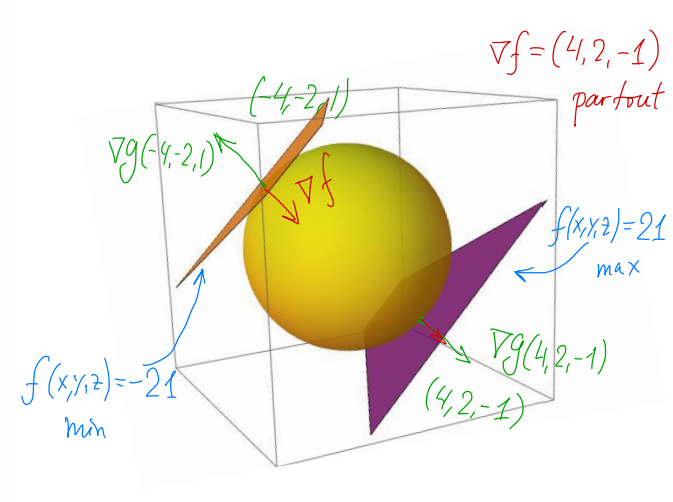
\includegraphics[scale=0.5]{12025-05-07.png}
    \end{center}
    Ici on a des plans qui sont en pente car on a notre plan  qui est ``pas tout joli'' ces plan veulent dire que notre fonction a toujours la même valeur dans ce point, et donc notre valeur a toujours la même valeur sur ce plan ce qui ``fausse'' notre idée d'un plan horizontale
    
\end{parag}
\begin{parag}{Example 2}
    Trouver les extrema de la fonction $f\left(x, y, z\right) =  xyz$ sous les contraintes 
    \begin{align*} \begin{cases}
        g_1\left(x, y, z\right) = x + y + z - 5 =  0\\
        g_2\left(x, y, z\right) =  xy + yz + xz - 8 =  0
    \end{cases} \end{align*}
    On va donc chercher:
    \begin{align*} \nabla g_1 \left(x, y, z\right) =  \left(1, 1, 1\right) \forall \left(x, y, z\right) \in \mathbb{R}^{3}\; \; \; \; \nabla g_2 \left(x, y, z\right) =  \left(y + z , x + z, x + y\right) \; \forall \left(x, y, z\right) \in \mathbb{R}^{3} \end{align*}
    On va donc chercher:
    \begin{align*} \nabla g_2\left(x, y, z\right) =  k \nabla g_1\left(x, y, z\right) \implies \left(y + z, x + z, x + y\right) = \left(k, k, k\right) \implies x =  y = z \end{align*}
    Et donc si on remplace ce que l'on vient de trouver dans notre fonction $g$:
    \begin{align*} 
        \begin{case}
            g_1\left(x, x, x\right) =  3x - 5 = 0 \implies x =  \frac{5}{3}\\
            g_2\left(x, x, x\right) =  3x^2 - 8 = 0 \implies 3\left(\frac{5}{3}\right)^2 =  \frac{25}{3} \neq 8
        \end{case}
    \end{align*}
    Ce qui implique donc que $\nabla g_1\left(x, y, z\right)$ et $\nabla g_2\left(x, y, z\right)$ sont linéairement indépendants ce qui implique que le théorème de Lagrange est applicable.\\
    Et donc obtient donc les équations:
\begin{align*}
    \begin{case}
        \nabla f\left(x, y, z\right) =  \left(yz, xz, xy\right) =  \lambda_1\left(1, 1, 1\right) + \lambda_2 \left(y + z, x + z, x + y\right)\\
        g_1\left(x, y, z\right) =  x + y + z - 5 =  0\\
        g_2\left(x, y, z\right) =  xy + yz + xz - 8 = 0
    \end{case}
\end{align*}
Ce qui nous donne:
\begin{align*} 
    \begin{case}
        yz =  \lambda_1 + \lambda_2 \left(y + z\right)\\
        xz =  \lambda_1 + \lambda_2\left(x + z\right)\\
        xy =  \lambda_1 + \lambda_2\left(x + y\right)\\
        x + y + z = 5\\
        xy + yz + xz =  8
    \end{case}
\end{align*}
Donc on voit ici que ça a l'air embêtant à faire donc on va se poser quelque minute pour voir s'il y a quelque chose afin d'accélérer tout ça.\\
Si on additionne nos deux première relations: 
\begin{align*} \left(1\right) + \left(2\right) \implies z\left(x + y\right) =  2\lambda_1 + \lambda_2\left(x + y + 2z\right)\\
    z\left(5-z\right) =  2\lambda_1 + \lambda_2\left(5 + z\right)
\end{align*}
On obtient donc une équation quadratique pour $z$.\\
Si on additionne $\left(2\right) + \left(3\right)$:
\begin{align*} x\left(5-x\right) =  2\lambda_1 + \lambda_2\left(5 + x\right) \end{align*}
Et finalement pour $\left(1\right) + \left(3\right)$:
\begin{align*} y\left(5-y\right) = 2\lambda_1 + \lambda_2\left(5 + y\right) \end{align*}
Ce qui revient donc:
\begin{align*} 
    \begin{case}
        z^2 + \left(\lambda_2 - 5\right)z + 5\lambda_2 + 2\lambda_1 =  0\\
        x^2 + \left(\lambda_2 - 5\right)x + 5\lambda_2 + 2\lambda_1 = 0\\
        y^2 + \left(\lambda_2 - 5\right) y + 5\lambda_2 + 2\lambda_1 = 0
    \end{case}
\end{align*}
Vu qu'on a trois fois la même équations; soit $x= y= z$ qui ne satisfait pas les contraintes, soit une variable différente des $2$ autres, par exemple $x =  y, z \neq x$.\\
On peut maintenant utiliser les équations (4) et (5):
\begin{align*} 
    \begin{case}
        2x + z =  5\\
        x^2 + 2xz =  8
        \end{case} \implies \begin{case} z = 5 - 2x\\ x^2 + 2x\left(5-2x\right) - 8 =  0 \implies 3x^2 + 10x - 8 = 0\end{case}
\end{align*}
Donc on peut résoudre notre équation tel que:

\begin{align*} 
    x = \frac{10 \pm \sqrt{100 - 96}}{6} =  \frac{10 \pm 2}{6} \\
    \implies x_1 =  2 =  y_1 \implies z_1 =  1\\
    \implies x_2 =  \frac{4}{3} =  y_2 \implies z_2 =  \frac{7}{3}
\end{align*}
Donc ici les points qu'on a trouvé sont:
\begin{align*} \left(x, y, z\right) =  \left(2, 2, 1\right), \left(1, 2, 2\right), \left(2, 1, 2\right)\\
\left(\frac{4}{3}, \frac{4}{3}, \frac{7}{3}\right), \left(\frac{7}{3}, \frac{4}{3}, \frac{4}{3}\right), \left(\frac{4}{3}, \frac{7}{3}, \frac{4}{3}\right)\end{align*}
Qui sont donc nos 6 points candidats. Donc il suffit maintenant de trouver on faisant les calculs:
\begin{align*} 
    f\left(2, 2, 1\right) =  f\left(1, 2, 2\right) =  f\left(2, 1, 2\right) =  4\\
f\left(\frac{4}{3}, \frac{4}{3}, \frac{7}{3}\right) = f\left(\frac{7}{3}, \frac{4}{3}, \frac{4}{3}\right) =f \left(\frac{4}{3}, \frac{7}{3}, \frac{4}{3}\right) = \frac{112}{3}
\end{align*}
Puisque les $g_1\left(x, y, z\right) =  0$, $g_2\left(x, y, z\right)$ est compact dans $\mathbb{R}^{3}$ et $f$ est continue. Alors $f$ atteint son min et son max sur le  compact; $f$ est de classe $c^{\infty}$ alors $f$ atteint son max, min, aux points donnés par notre calcul.\\
\begin{subparag}{remarque}
    Ici il faudrait aussi prouver que le sous-ensemble soit compact
\end{subparag}

\end{parag}
\section{Résumé: Méthode de démonstration}
\begin{parag}{Démonstration direct}
   \begin{align*} P \implies Q \end{align*}
   A base de logique tel que:
   \begin{align*} P \implies \ldots \implies Q \end{align*}
\end{parag}
\begin{parag}{Par contraposée}
   \begin{align*} P \implies Q \end{align*} 
   On le prouve tel que :
   \begin{align*} \neg Q \implies \ldots \implies \neg P \end{align*}
\end{parag}
\begin{parag}{Disjonction des cas}
    \begin{align*} P \implies Q \end{align*}
    On le fait par cas:
    \begin{align*} 
        P = \begin{case}
            \text{cas 1} \implies Q\\
            \vdots\\
            \text{ cas n} \implies Q
        \end{case}
    \end{align*}
\end{parag}

\begin{parag}{Si et seulement si}
    \begin{align*} \iff \end{align*}
\end{parag}

\begin{parag}{Par récurrence}
   \begin{align*} P\left(n\right) \end{align*} 
   \begin{subparag}{Simple}
       \begin{itemize}
           \item \textbf{Base}: $P\left(n_0\right)$
           \item \textbf{Hérédité}: $P\left(n\right) \implies P\left(n+1\right)$
       \end{itemize}
   \end{subparag}
   \begin{subparag}{Généralisé}
       \begin{itemize}
           \item \textbf{Base}: $P\left(n_0\right), \ldots, P\left(n_0 + k\right)$
           \item \textbf{Hérédité}: $\left\{P\left(n\right), \ldots, P\left(n + k\right)\right\} \implies P\left(n+k+1\right)$
       \end{itemize}
   \end{subparag}
   \begin{subparag}{Forte}
       \begin{itemize}
           \item \textbf{Base}: $P\left(n_0\right)$
           \item \textbf{Hérédité}: 
       \end{itemize}
       
   \end{subparag}
\end{parag}











\begin{parag}{Exemple: choisir la méthode de démonstration}
    \begin{subparag}{Proposition 1}
        Pour tout $n \in \mathbb{N}$, $2n^2 + n + 1$ n'est pas divisible par $5$.
    \end{subparag}
    \begin{subparag}{Question 2}
        Il y a 12 boules vertess, $15$ boules rouges et 16 boules blanches dans un sac, Quel nombre minimal de boules faut-il sortir du sac pour avoir au moins $4$ boules de même couleur?
    \end{subparag}
    \begin{subparag}{Proposition 3}
            Il existe une infinité de nombre premier tels que:
            $p + 2$ n'est pas premier.
    \end{subparag}
    \begin{subparag}{Proposition 4}
        Il n'existe pas de nombre entiers $x, y$ tels que $42x - 70 y =  124$
    \end{subparag}
    \begin{subparag}{Proposition 5}
        Pour tout $n \geq 2$ naturel, on a:
        \begin{align*} P\left(n\right): \prod_{k = 2}^{n} \left(1- \frac{1}{k^2}\right)  \end{align*}
    \end{subparag}
    \begin{subparag}{Proposition 6}
        Si $f: \mathbb{R}^{3} \to \mathbb{R}$ de classe $C^2$, telle que $\det $ Hes$s_f\left(\overline{0}\right) < 0$, Alors $\overline{0}$ n'est pas un point de minimum local de $f$
    \end{subparag}
    \begin{subparag}{Proposition 7}
        Soient $x, y \in \mathbb{R}$. Si $y^3 + yx^2 - x^3 \leq xy^2$, alors $y \leq x$
    \end{subparag}
\end{parag}
\begin{parag}{Méthode}
    
    \begin{subparag}{Proposition 1}
        Pour cette méthode on va plutôt utilise la disjonction des cas comme la plupart des propositions avec la divisibilité
    \end{subparag}
    \begin{parag}{Question 2}
        Ici on utilise Les tiroirs car un a un nombre ``minimale'' qui peut facilement se compter.
    \end{parag}
    
    \begin{subparag}{Proposition 3}
        On utilise l'absurde avec le Euclide\\
        On prends un premier $q$ premier quelque part tel que $q + 2$ est premier néanmoins si on prends donc $q\left(q+2\right)$ est un nombre qui rentre dans la contradiction.
    \end{subparag}

    \begin{subparag}{Proposition 4}
        Donc ici on fait par l'absurde tel que ``imaginons que cela existe'' on voit que cela est une contradiction, donc cela ne peut pas exister.
    \end{subparag}
    \begin{subparag}{Proposition 5}
        
    \end{subparag}
    \begin{subparag}{Proposition 6}
        Ici on peut juste faire une preuve direct
    \end{subparag}
    \begin{subparag}{Proposition 7}
        Ici on utilise la contraposée 
    \end{subparag}
\end{parag}



\begin{parag}{Question}
    Soit une famille des propostions $\left\{P\left(n\right)\right\}_{n \in \mathbb{N}}$, telle que, pour tout $n \in \mathbb{N}$, si $P\left(n\right)$ est vraie, alors $P\left(n+4\right)$ est vraie.\\
    Alors:
    \begin{enumerate}
        \item $P\left(6\right)$ et $P\left(8\right)$ ne peuvent pas être vrai les deux
        \item si $P\left(19\right)$ est vrai, alors $P\left(7\right)$ est vraie
        \item $P\left(2\right)$ et $P\left(10\right)$ sont soit les deux vraies, soit les deux fausses
        \item si $P\left(21\right)$ est fausse, alors $P\left(9\right)$ est faux
    \end{enumerate}
    

\end{parag}


\chapter{Calcul d'intégrale des fonctions de plusieurs variables}
\lecture{23}{2025-05-12}{Intégrale à plusieurs variables}{}

\section{Intégrale sur un pavé fermé}
\begin{definition}
    Un \important{pavé fermé} est un sous-ensemble de $\mathbb{R}^{n}$ qui est le produit cartésien de $n$ intervalles fermés bornés:
    \begin{align*} P =  \left[a_1, b_1\right] \times \ldots \times \left[a_n b_n\right] \; \; a_i < b_i \forall i = 1, \ldots, n\end{align*}
    On note le pavé ouvert $\mathring{P} =  ] a_1, b_1 [ \times \ldots \times ] a_n b_n [$
\end{definition}


\begin{parag}{Exemple}
    Pour un pavé de dimension $1$ , $P_1 =  \left[a, b\right]$ qui est juste un intervalle fermé.\\
    Pour un pavé de dimension $2$ $\implies P_2 = \left[a_1, b_1\right] \times \left[a_2, b_2\right]$
\end{parag}
\begin{parag}{Volume d'un pavé fermé}
    \begin{definition}
        Le volume d'un pavé fermé set défini par:
        \begin{align*} \left|P\right| =  \left(b_1 - a_1\right)\left(b_2 - a_2\right) \cdot  \ldots \cdot  \left(b_n - a_n\right) \end{align*}
    \end{definition}
    
    \begin{definition}
        Soit $G_j$ une \important{sbdivision} de $\left[a_j, b_j\right]; a_j < b_j$ tel que
        \begin{align*} G_j =  \left\{a_j =  x_0^i < x_1^j < \ldots < x_{n_j}^j < b_j\right\} \end{align*}
        Alors $G = \left(G_1, \ldots, G_n\right)$ est appelée une \important{subdivision de $P$}
    \end{definition}

\end{parag}
\begin{parag}{Somme de Darboux}
    \begin{definition}
        Soit $f: P \to \mathbb{R}$ \important{bornée sur $P$} Alors on définit \important{les sommes de Darboux} de $f$ sur $P$.\\
        Soit $D\left(\sigma\right)$ une collection des pavées fermés engendrée par la subdivision $\sigma$.\\
        Alors $S_{\sigma}\left(f\right) =  \sum_{Q \subset D\left(\sigma\right)}m\left(Q\right)\left|Q\right| $ où $m\left(Q\right) =  \text{inf}_{\overline{x}\in Q}f\left(\overline{x}\right)$\\
        $\overline{S}_{\sigma} =  \sum_{Q \subset D\left(\sigma\right)} M\left(Q\right) \left|Q\right| $ où $M\left(Q\right) =  \text{sup}_{\overline{x}\in Q}f\left(\overline{x}\right)$\\
        Alors $S\left(f\right) = \text{sup}\{S_{\sigma}\left(f\right)$, $\sigma$ est une subdivision de $P \}$ est la somme de Darboux.\\

    \end{definition}
\end{parag}
\begin{parag}{Integrabilité}
    \begin{definition}
        Soit $P \subset \mathbb{R}^{n}$ une pavé fermé et $f: P \to \mathbb{R}$ une fonction bornée. Alors,  $f$ est \important{intégrable sur $P$} si et seulement si:
        \begin{align*} S\left(f\right) =  \overline{S}\left(f\right)  \end{align*}
        Pour lesquels on a toujours $S\left(f\right) \leq \overline{S} \left(f\right)$\\
        Dans ce cas, \important{l'integrale de $f$ sur $P$} est définie par:
        \begin{align*} \int \int \int \int_P f\left(\overline{x}\right) d\overline{x} =  \int_P \int\ldot\s\int f\left(x_1, \ldots, x_n\right) dx_1 \ldots dx_n =  S\left(f\right) =  \overline{S}\left(f\right) \end{align*}
    \end{definition}
\end{parag}
\begin{parag}{Exemple $3$}
    Soit $P \subset \mathbb{R}^{n}$ un pavé fermé: $f: P \to \mathbb{R}$, $f\left(\overline{x}\right) =  C \in \mathbb{R}$ constante.\\
    Soit $\sigma$ une subdivision de $P$. $S_{\sigma}\left(f\right) =  \sum_{Q \in D\left(\sigma\right)} \text{inf}_Q\left(f\right)\left|Q\right| =  C \sum_{Q}\left|Q\right|= C \left|P\right| $
\end{parag}

\begin{parag}{Quelque exemple}
    Soit $f\left(\overline{x}\right) =  1$ Alors:
    \begin{align*} \int_P d\overline{x} =  \int\int\ldot\s\intdx_1, \ldots dx_n \end{align*}
\end{parag}

\begin{parag}{Théorème}
    \begin{theoreme}
        Toute fonction \important{continue} est \important{intégrable} sur \important{un pavé fermé}.
    \end{theoreme}
    \begin{subparag}{Idée de la preuve}
        Soit $f : P \to \mathbb{R}$ une fonction continue.\\
        En premier lieu, $f$ est bornée sur $P$. Puisque $P$ est un sous-ensemble compact. Alors cette fonction atteint son minimum et maximum sur $P \implies f$ est bornée sur $P$.\\
        Soit $\epsilon > 0$ si $f$ est continue en chaque point de $P$. Cela implique que:
        \begin{align*} \forall \overline{x}_0 \in P\;\; \exists \delta_{\overline{x}_0}  : \left|\left|\overline{x}_0 - \overline{x}\right|\right|< \delta_{\overline{x}_0} \implies \left|f\left(\overline{x}\right) - f\left(\overline{x}_0\right)\right| \leq \frac{\epsilon}{2}\end{align*}
        On considère le recouvrement de $P$ pour des boules ouvertes $B\left(\overline{x}_0, \sigma_{\overline{x}_0}\right)$ Ce qui implique par le théorème de Heine-Borel_Lebesgue que parce que c'est un recouvrement fini, on a une subdivision fini $\sigma$ ce qui implique que $\overline{S}_{\sigma} - S_{\sigma} \leq \epsilon\left|P\right| \implies \overline{S} - S \leq \epsilon \left| P\right|$ Ce qui implique finalement que $f$ est intégrable sur $P$.
    \end{subparag}
\end{parag}
\begin{parag}{Propriétés de l'intégrale}
    \begin{enumerate}
        \item \textbf{Additivité}: Soit $P$ un pavé fermé et $\left\{P_i\right\}_{i \in I}$ une famille finie (dénombrable) des pavés fermés tels que $P =  \bigcup_{i \in I}P_i$ \\
            Alors pour toute fonction continue $f: P \to \mathbb{R}$ on a:
            \begin{align*} \int_P \end{align*}

    \end{enumerate}
    
\end{parag}
\subsection{Théorème de Fubini sur un pavé fermé}
\begin{theoreme}
    Soit $f: P \to \mathbb{R}$ continue, $P =  \left[a_1, b_i\right] \times \ldots \times \left[a_n, b_n\right]$\\
    Alors $f$ est intégrable sur $P$ et on a:
    \begin{align*} \int_P f\left(\overline{x}\right)d\overline{x} = \int_{a_n}^{b_n}\left(\int_{a_{n-1}}^{b_{n-1}}\ldots \left(\int_{a_1}^{b_1} f\left(x_1, \ldots, x_n\right)dx_1\right)dx_2\ldots dx_{n-1}\right)dx_n \end{align*}
\end{theoreme}
\begin{parag}{Explication}
    Donc en fait on intègre une variable à la fois avec les autres $x_j$ comme paramètre.  On commence de l'intérieur  jusqu'à l'extérieur (Cela est fait pour le théorème de Fubini, néanmoins on peut quand même échanger l'ordre des variables dans l'intégrale). \important{Attention},  cela ne fonction seulement sur un pavé fermé.\\

\end{parag}









\lecture{24}{2025-05-14}{Intégrale sur un domaine borné}{}
\begin{parag}{Example avec le théorème de Fubini}
    Le but ici est de calculer le volume du sous-ensembe de  $\mathbb{R}^{3}$ défini par:
    \begin{align*} \left\{\left(x, y, z\right) in \mathbb{R}^{3}: 0 \leq x \leq 4, 0 \leq y \leq 3, 0 \leq z \leq \left( 1 + 3x + x\sin\left(xy\right)\right)\right\} \end{align*}
    \begin{framedremark}
        La fonction $1 + x\left(3 + \sin\left(xy\right)\right) > 0$ et elle est continue.
    \end{framedremark}
    Donc on a que $P =  \underbrace{\left[0, 4\right]}_{x} \times \underbrace{\left[0, 3\right]}_{y}$.\\
    On calcule dont le volume $V =  \int_\P\int \left(1 + 3x + x\sin\left(xy\right)\right)dxdy$ Qui par la linéarité nous donne:

    \begin{align*}  
        V &= \int_\P\int 1dxdy + 3\int\int_Pxdxdy + \int\int_Px\sin\left(xy\right)dxdy\\
          &= 1\cdot \overbrace{1\left(4-0\right)\left(3-0\right)}^{= 12} + 3 \int_0^5\left(\int_0^4 xdx\right)dy + \int\int_px\sin\left(xy\right)dxdy 
    \end{align*}
    Pour la deuxième intégrale on a:
    \begin{align*} 3\int_0^5\left(\int_0^4xdx\right)dy = 3\int_0^31dy\cdot \int_0^4xdx\\
    = 3y_{0 \to 3}\cdot \frac{1}{2}x^2_{0 \to 4} =  9 \cdot  8 =  72\end{align*}
    Pour la dernière intégrale on a:
    \begin{align*} \int\int_P x \sin\left(xy\right)dxdy &=  \int_0^4\left(\int_0^3x\sin\left(xy\right)dy\right)dx =  \int_0^4\left(\int_0^3 \sin\left(xy\right)d\left(xy\right)\right)dx\\
    &= \int_0^4 - \cos\left(xy\right)_{0 \to 3}dx\\
    &= \int_0^4 \left(-\cos\left(3x\right) +\right) 1 dx =  -\frac{1}{3}\sin\left(3x\right) + x_{0 \to 4} =  -\frac{1}{3}\sin\left(12\right) + 4
\end{align*}
Ce qui nous donne pour le volume final: $V =  12 + 72 - \frac{1}{3}\sin\left(12\right) =  88 - \frac{1}{3}\sin\left(12\right)$.
\end{parag}
\begin{parag}{Dans l'autre sens}
    On peut considérer la même intégrale  dans l'autre sens $\int_0^3\left(\int_0^4 x \sin\left(xy\right)dx\right)dy$\\
    Pour résoudre cela on va faire une intégration par partie ce qui nous donne:
    \begin{align*} 
        \int_0^4 x \sin\left(xy\right)dx =  -\int_0^4\frac{x}{y}d\left(\cos\left(xy\right)\right) 
    \end{align*}
    \begin{align*} 
        = - \frac{x\cos\left(xy\right)}{y}_{0\to 4} + \int_0^4 \cos\left(xy\right) \cdot  \frac{1}{y}dx\\
        = -\frac{4\cos\left(4y\right)}{y} + \frac{1}{y^2}\sin\left(xy\right)_{0 \to 4} = -\frac{4\cos\left(4y\right)}{y} + \frac{\sin\left(4y\right)}{y^2}
    \end{align*}
    Nous voyons que cette fonctions n'est pas définie en $0$ si l'on veut éviter de faire une intégrale impropre, ça peut être rentable d'essayer de prolonger la fonction en $y = 0$:\\
    Par un développement limité de sinus:
    \begin{align*} 
        \lim_{y  \to 0} \frac{\sin\left(4y\right) - 4y\cos\left(4y\right)}{y^2} =  \lim_{y \to 0} \frac{4y - \frac{1}{6}\left(4y\right)^3 + \ldots - 4y\left(1 - \frac{1}{2}\left(4y\right)^2^+ \ldots \right)}{y^2} \\
        = \lim_{y \to 0} \frac{C\left(y^3\right)}{y^2} =  0
    \end{align*}
    On a donc que:
    \begin{align*} 
        \int_0^3 \frac{\sin\left(4y\right) - 4y\cos\left(4y\right)}{y^2}dy = \int_0^3 \frac{\sin\left(4y\right)}{y^2}dy - \int_0^3 \frac{4y\cos\left(4y\right)}{y^2} dy
    \end{align*}
    Néanmoins ces primitives ne s'expriment pas en fonctions élémentaires. Pour quand même essayer de trouver un résultat convaincant, on peut en tirer des sommes:\\
L'idée ici c'est d'utiliser le faite que la dérivée de $\frac{1}{y}$ est $\frac{-1}{y^2}$:
    \begin{align*} 
        \int_0^3 \frac{\sin\left(4y\right)-4y\cos\left(4y\right)}{y^2} dy &= \int_0^3\left(4y\cos\left(4y\right)-\sin\left(4y\right)\right)d\left(\frac{1}{y}\right)\\
            &= -\frac{\sin\left(4y\right)}{y} + 4\cos\left(4y\right)_{0 \to 3} - \int \frac{4\cos\left(4y\right) - 16y\sin\left(4y\right) - 4\cos\left(4x\right)}{y} dy\\
            &= -\frac{\sin\left(12\right)}{3} + 4\cos\left(12\right) + \lim_{x \to 0} \frac{\sin\left(4y\right)}{y} - 4 + \int_0^3 16\sin\left(4y\right)dy\\
            &= -\frac{\sin\left(12\right)}{3} + 4\cos\left(12\right) + 4 - 4 -4\cos\left(4y\right)_{0 \to 3}\\
            &= -\frac{\sin\left(12\right)}{3} + 4\cos\left(12\right) - 4 \cos\left(12\right) + 4\\
            &= 4- \frac{1}{3}\sin\left(12\right)
    \end{align*}
    Qui est le même résultat que l'intégrale précédente.
    
    \begin{subparag}{Conclusion}
        Il est important donc de choisir un bonne ordre pour l'intégration afin d'éviter des calculs techniques
    \end{subparag}
\end{parag}


\subsection{Intégrale sur un domaine bornée}
\begin{parag}{Définition}
    \begin{definition}
        Soit $E \subset P \subset \mathbb{R}^{n}$; $f: E \to \mathbb{R}$ fonction bornée sur $E$.\\
        Posons $\bhat{f}\left(\overline{x}\right) =  \begin{cases} f\left(\overline{x}\right), \overline{x} \in E\\ 0, \overline{x} \in P \setminus E \end{cases}$ La fonction $f$ est intégrable sur $E$ si $\bhat{f}$ est intégrable sur $P$.
    \end{definition}
    Dans ce cas on pose: 
    \begin{align*} \int_E f\left(\overline{x}\right) d\overline{x} =  \int_P \bhat{f}\left(\overline{x}\right) d\overline{x} \end{align*}
\end{parag}
\begin{parag}{Remarque}
    \begin{enumerate}
        \item La définition ne dépends pas du choix du pavé fermé autour de $E$.
        \item Condition suffisante d'intégrabilité. Si $f : E \to \mathbb{R}$ est bornée sur $E$, continue sur $\overline{E}$et la frontier $\partial E$ est aussi régulière ( de mesure nulle)
    \end{enumerate}
    $\implies $ Alors, $f\left(\overline{x}\right)$ est intégrable sur $E$.
    \begin{subparag}{Frontière régulière}
         \begin{definition}
            \begin{align*} 
                \forall \epsilon > 0\; \; \exists \text{ un recouvrement } \partial E \subset \bigcup_{i \in I}q_i\; , q_i \text{ pavés fermés} \\\text{ tels que } \sum_{i \in I}\left|q_i\right| < \epsilon
                \implies \partial E \text{ est de mesure nulle }
            \end{align*}
         \end{definition}
         \begin{align*}
            
         \end{align*}
    \end{subparag}
    
\end{parag}


\begin{parag}{Théorème de Fubini sur un domaine régulier}
   \begin{theoreme}
    \begin{enumerate}
        \item Soit $\left[a, b\right] \subset \mathbb{R}$, un intervalle, $a < b$
        \item $\phi_1, \phi_2: \left[a, b\right] \to \mathbb{R}$ fonction continues, telles que
            \begin{align*} \phi_1\left(x\right) y \phi_2\left(x\right) \; \forall x \in ] a, b [ \end{align*}
            Soit $D =  \left\{\left(x, y\right) \in \mathbb{R}^{2}: a < x < b, \phi_1\left(x\right) < y < \phi_2\left(x\right)\right\}$, Alors pour toute fonction continue $f: \overline{D} \to \mathbb{R}$ on a:
            \begin{align*} 
                \int_D \int f\left(x, y\right)dxdy = \int_a^b\left(\int_{\phi_1\left(x\right)}^{\phi_2\left(x\right)}f\left(x, y\right) dy\right)dx
            \end{align*}
            \begin{center}
                \includegraphics[scale=1.1]{12025-05-14.png}
            \end{center}
            
        \item Soit $\left[c, d\right] \subset \mathbb{R}$, un intervalle $c < d$\\
            $\psi_1, \psi_2 : \left[c, d\right] \to \mathbb{R}$ des fonctions continues telles que
            \begin{align*} \psi_1\left(y\right) < \psi_2\left(y\right)\; \; \forall y \in ] c, d [ \end{align*}
            Soit $D =  \left\{\left(x, y\right) \in \mathbb{R}^{2}c < y < d, \psi_1\left(y\right) < x < \psi_2\left(y\right)\right\}$ \\
            Alors pour toute fonction continue $f: D \to \mathbb{R}$ on a
            \begin{align*} \int_D \int f\left(x, y\right)dxdy = \int_c^d\left(\int_{\psi_1\left(y\right)}^{\psi_2\left(y\right)} f\left(x, y\right)dx\right)dy \end{align*}
    \end{enumerate}
    \begin{center}
        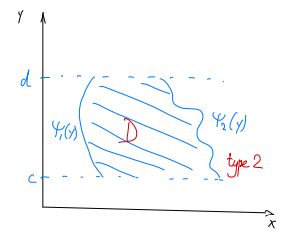
\includegraphics[scale=1.1]{22025-05-14.png}
    \end{center}
   \end{theoreme} 
\end{parag}

\begin{parag}{Exemple}
    Soit $D =  \left\{\left(x, y\right) \in  \mathbb{R}^{2}: 0 < x < 1, 0 < y < 2-2x\right\}$, avec $f\left(x, y\right) =  xy$. On a D de type $1$.\\
    \begin{align*} 
        D =  \left\{\left(x, y\right) \in \mathbb{R}^{2}, 0 < x < 1, \phi_1\left(x\right)< y < \phi_2\left(x\right)\right\}
    \end{align*}
    Avec $\phi_1\left(x\right) =  0, \phi_2\left(x\right) =  2 - 2x$ On a alors l'intégrale:
    \begin{align*} 
        \int_D\int xy dxdy &=  \int_0^1\left(\int_0^{2-2x} xydy\right)dx\\ &=  \int_0^1x \frac{1}{2}y^2 \mid_{0}^{2-2x} dx\\
        &= \frac{1}{2}\int_0^1x\left(2-2x\right)^2dx \\ &=  2 \int_0^1x\left(1-x\right)^2 dx\\ &=  2\int_0^1x\left(1-2x + x^2\right) dx\\ &=  2\int_0^1 \left(x-2x^2 + x^3\right) dx\\
        &= 2\left(\frac{1}{2}x^2 - \frac{2}{3}x^3 + \frac{1}{4}x^4\right)\mid_0^1 =  \frac{1}{6}
    \end{align*}
    Néanmoins on peut aussi le voir comme $D$ de type $2$: $D = \left\{\left(x, y\right) \in \mathbb{R}^{2}: 0 < y < 2, 0 < x < 1 - \frac{1}{2}y\right\}$ , on a donc pour nos deux fonctions $\psi_1\left(y\right) = 0$ et $\psi_2\left(y\right) = 1 - \frac{1}{2}y$. Ce qui nous donne:
    \begin{align*} 
        \int_D \intxydxdy =  \int_0^2\left(\int_{\psi_1\left(y\right)}^{\psi_2\left(y\right)}xy dx\right) dy\\
        = \int_0^2\left(\int_0^{1 - \frac{1}{2}y}xydx\right)dy 
    \end{align*}
    Intégral à faire à la maison.
\end{parag}
\begin{parag}{Si le domaine $D$ n'est pas de type 1 ou 2?}
    Donc si on a par exemple la fonction:
    \begin{center}
        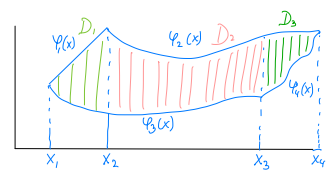
\includegraphics[scale=0.7]{32025-05-14.png}
    \end{center}
    
    Pour pouvoir intégrer, il faut diviser le domaine en réunions de domaines de type 1  ou 2 et utiliser l'additivité de l'intégrale. tel que $D$ est:
    \begin{align*} D =  \bigcup_{i =  1}^3 D_i \end{align*}
\end{parag}
\begin{parag}{Exemple 2}
    $D =  \left\{\left(x, y\right) \in \mathbb{R}^{2} : 0 \leq x \leq \sqrt{4 - y^2}, y \leq x\right\}$, on demande de calculer $\int\int_D \frac{x}{4 + y^2}dxdy$.\\
    Donc en premier lieu on va devoir regarde notre domaine $D$. On a en premier lieu $x =  \sqrt{4-y^2} \implies x^2 + y^2 =  4$ qui est donc un cercle.m pour $0 \leq x \leq \sqrt{4-y^2}$ on a donc quon est dans le cercle mais que $x \geq 0$ ce qui nous dit qu'on prends le demi cercle à fauche. Finalement, on a que $y \leq x$ qui est tout ce qui se trouve en dessous de la droite. On a donc le demi Cercle à droite de $x =  0$ qui se trouve en dessous de la droite $y = x$. On peut découper cela en deux domaines\\
    Ecrivons donc le premier domaine du quart de cercle en bat à droite:
    \begin{align*} D_1 = \left\{-2 < y < 0, 0 < x < \sqrt{4-y^2}\right\} \end{align*}
    On a donc pour le deuxieme domaine:
    \begin{align*} 
        D_2 = \left\{0 < y < \sqrt{2}, y < x < \sqrt{4 - y^2}\right\}
    \end{align*}
    On a donc l'intégrale
    \begin{align*} 
        I &= \int_{-2}^0\left(\int_0^{\sqrt{4-y^2}}\frac{x}{4 + y^2}dx\right)dy + \int_0^{\sqrt{2}}\left(\int_y^{\sqrt{4-y^2}}\frac{x}{4 + y^2}dx\right)dy\\
          &= \int_{-2}^0\frac{1}{2}\left(\frac{4-y^2}{4 + y^2}\right)dy + \int_0^{\sqrt{2}}\frac{1}{2}\frac{4-y^2 - y^2}{4 + y^2}dy\\
          &= \frac{1}{2}\int_{-2}^0\frac{-4 - y^2 + 8}{4 + y^2}dy + \frac{1}{2}\int_0^{\sqrt{2}} \frac{-2\left(4 + y^2\right) + 12}{4 + y^2} dy\\
          &= \frac{1}{2} \int_{-2}^0\left(-1 + \frac{8}{4 + y^2}\right)dy + \frac{1}{2}\int_0^{\sqrt{2}}\left(-2 + \frac{12}{4+y^2}\right)dy\\
          &= -\frac{1}{2}y \mid_{-2}^0 + \int_{-2}^0 \frac{4}{4 + y^2}dy - y \mid_0^{\sqrt{2}} + \frac{3}{2}\int_{0}^{\sqrt{2}}\frac{4}{4 + y^2}dy\\
          &= - 1 + 2\int_{-2}^0 \frac{1}{1 + \left(\frac{y}{2}\right)^2}d\left(\frac{y}{2}\right) - \sqrt{2} + \frac{3}{2} 2\int_0^{\sqrt{2}} \frac{1}{1 + \left(\frac{y}{2}\right)^2} d\left(\frac{y}{2}\right) =  - 1 + 2 \arctan \left( \frac{y}{2}\right)\mid_{-2}^0 - \sqrt{2} + 3\arctan\left(\frac{y}{2}\right) \mid_0^{\sqrt{2}}\\
          &= - 1 - \sqrt{2} + -2\left(\frac{\pi}{4}\right) + 3 \arctan\left(\frac{\sqrt{2}}{2}\right) \\
          &= -1 - \sqrt{2} + \frac{\pi}{3} + \underbrace{3\arctan\left(\frac{\sqrt{2}}{2}\right)}_{\approx 0,615} > 0
    \end{align*}

\end{parag}


\begin{parag}{Remarque: calcul d'aire d'un domaine dans $\mathbb{R}^{2}$}
    Soit $D \subset \mathbb{R}^{2}$ un sous-ensemble regulier, Alors on peut calculer l'aire $D$ par intégration double comme suit:
\end{parag}
\begin{parag}{Question}
    L'aire du domaine $D$ entre les courbes $y =  -x^2 + 2x +  1$ et $y = 1 - x$ est donné par l'intégrale:\\
    On domaine juste d'écrire l'intégrale mais pas de la résoudre (on utilise ici le type 2).
    

\end{parag}

petit test



\lecture{25}{2025-05-19}{Intégrales sur intégrales}{}


\begin{parag}{Exemple}
	$D = \left\{(x, y) \in \mathbb{R}^{2}: 1 < x < 2, \frac{1}{x} < y  < x \right\}$ avec la fonction $f\left(x, y\right) = x + \frac{1}{y}$ Nous cherchons donc:
	\begin{align*} \int\int_D f(x, y)dxdy = ? \end{align*}
	Comme on peut le voire, notre ensemble est dejà une intégrale de type 1. On obtient:
	\begin{align*} \int_1^2 \left( \int_{\frac{1}{x}}^x x + \frac{1}{y}dy \right) dx &= \int_1^2dx \int_{\frac{1}{x}}^x x + \frac{1}{y}dy\\
	&= \int_1^2dx (xy + \ln y)\mid_{\frac{1}{x}}^x\\
	&= \int_1^2 x^2 + \ln x - 1 - \ln \frac{1}{x} dx\\
	&= \int_1^2 x^2 + 2\ln x - 1 dx =  \frac{1}{3}x^3 - x \mid_1^2 + 2 \int_1^2 \ln x dx \\
	&= \frac{8}{3} -2 - \frac{1}{3} + 1 + 2x\ln x \mid_1^2 - 2\int 1dx\\
	&= \frac{7}{3} - 1 + 4\ln 2 - 2x\mid_1^2 = \frac{7}{3} - 1 + 4\ln 2 - 4 + 2 = -\frac{2}{3} + 4 \ln 2 > 0
	\end{align*}
\end{parag}

\begin{parag}{Changement d'ordre par intégration}
    Donc si maintenant on veut le faire dans l'autre sens, on veut écrire $x$ dans les bornes de $y$.\\
    On cherche en premier lieu l'intersection les deux intersections de $D: y = x$ et $y =  \frac{1}{x}$:
    \begin{align*} 
	    \frac{1}{x} =  x \implies x^2 = 1, x > 0 \implies x =  1, y = 1
    \end{align*}
    On a donc le max qui est $x =  2= y$ ce qui nous donne:
    \begin{align*} D_1 = \{1 < y < 2, \mathspace y < x < 2\}\\
	    D_2 =  \{\frac{1}{x} < y < 1, \frac{1}{y} < x < 2\}
    \end{align*}
    Qui sont donc les deux de types $2$. Si on écrit donc l'intégrae:
    \begin{align*} 
	    \int_{\frac{1}{2}}^1 \left(\int_{\frac{1}{y}}^2 x + \frac{1}{y}dx\right) dy + \int_1^2 \left(\int_y^2 x + \frac{1}{y}dx\right) dy
    \end{align*}
\end{parag}




\begin{parag}{Exemple 2}
	Soit $D = \{ \left(x, y\right) \in \mathbb{R}^{2}: 0 < y < 1, 0 < x < \arccos y\}$.\\
	Calculer $\int\int_D xdxdy \implies D = \{\left(x, y\right) \in\mathbb{R}^{2}:0 < x < \frac{\pi}{2}, 0 < y < \cos x\}$ Ce que l'on peut aisément intégrer:
	\begin{align*} 
		\int_0^{\frac{\pi}{2}}dx \int_0^{\cos x}xdy &= \int_0^{\frac{\pi}{2}}dx (xy\mid_0^{\cos x})\\
							    &= \int_0^{\frac{\pi}{2}}x \cos x dx = \int_0^{\frac{\pi}{2}} \underbrace{x}_{f}d \underbrace{\sin x}_{g}\\
							    &= x\sin x \mid_0^{\frac{\pi}{2}} - \int_0^{\frac{\pi}{2}}\sin x dx\\
							    &= \frac{\pi}{2} - 1
	\end{align*}
	Maintenant on peut le faire dans l'autre sens:
	\begin{align*} 
		\int\int_D x dxdy &= \int_0^1 dy \int_0^{\arccos y}xdx\\
				  &= \int_0^1 dx (\frac{1}{2}x^2 \mid_0^{\arccos y})\\
				  &= \frac{1}{2} \int_0^1 (\arccos y)^2 dy\\
				  &= \frac{1}{2}\int_{\frac{\pi}{2}}^0 u^2 d \cos u\\
				  &= \frac{1}{2} u^2 \cos u \mid_{\frac{\pi}{2}}^0 - \frac{1}{2}\int_{\frac{\pi}{2}}^0 2u \cos u du \\
				  &= 0 - \int_{\frac{\pi}{2}}^0 u d \sin u = -u \sin u\mid_{\frac{\pi}{2}}^0 - \int_{\frac{\pi}{2}}^0\sin u du = \frac{\pi}{2} - 1
	\end{align*}
	Comme on le voit ici, ça vaut la peine de refléchir quel type utiliser avant de commencer à calculer.
\end{parag}


\subsection{Théorème de Fubini pour les intégrales triples}
\begin{parag}{Théorème}
   \begin{theoreme}
	   Soit $\left[a, b\right]$ intervalle, $a < b$; $\phi_1, \phi_2: \left[a, b\right] \to \mathbb{R}$ continues $\phi_1\left(x\right) < \phi_2 \left(x\right) \forall x \in ] a, b [$.
	   \begin{align*} D = \left{(x, y) \in \mathbb{R}^{2}: a < x < b, \mathspace \phi_1(x) < y < \phi_2(x)\right} \end{align*}
	   Soient $G_1, H : \overline{D} \to \mathbb{R}$ continues, tel que $G\left(x, y\right) < H\left(x, y\right) \mathspace \forall \left(x, y\right) \in D$.\\
	   \begin{align*} E =  \{(x, y, z) \in \mathbb{R}^{3}: (x, y) \in D; \mathspace G(x, y) < z < H(x, y)\} \end{align*}
	   Soit $f : \overline{E} \to \mathbb{R}$ continue,\\
	   Alors $f$ est intégrable sur $E$ et on a:
	   \begin{align*} 
		   \int\int\int_E f(x, y, z) dxdydz =  \int_a^b \left(\int_{\phi_1(x)}^{\phi_2(x)}\left(\int_{G(x, y)}^{H(x, y)}f(x, y, z)dz\right)dy\right)dx
	   \end{align*}
   \end{theoreme} 
\end{parag}

\begin{parag}{Exemple}
	Soit $E = \{\left(x, y, z\right) \in \mathbb{R}^{3}: 0 < z < y < x < 1\} \implies \int\int\int_E f\left(x, y, z\right)dxdydz =$  Avec la fonction $f\left(x, y, z\right) = e^{x^3}$\\
	On cherche donc à écrire nous ensemble petit à petit. On sait déjà que $0 < x < 1$ et que $0 < y < x$, et que $0 < z < y$ (c'est comme si on séparait notre inégalité).
	Ce qui nous donne comme domaine:
	\begin{align*} E = {(x, y) \in \mathbb{R}^{3}, 0 < x < 1, 0 < y < x, 0 < z < y} \end{align*}
	\begin{center}
	    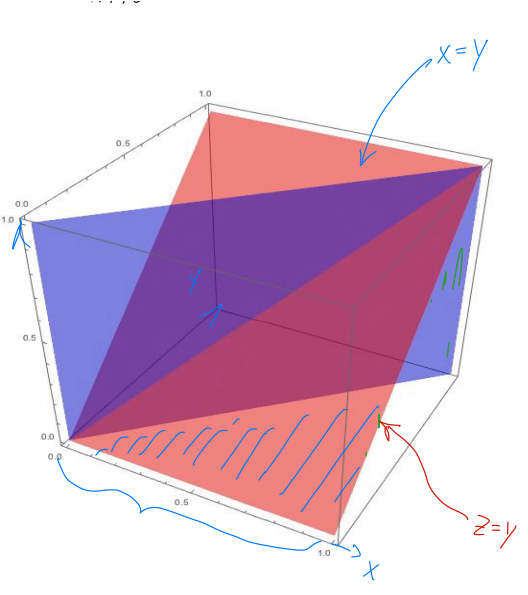
\includegraphics[scale=0.8]{12025-05-19.png}
	\end{center}
	

	On nous donne donc comme intégrale:
	\begin{align*} 
		\int\int\int_E f(x, y, z)dxdydz &= \int_0^1dx \int_0^x dy \int_0^y e^{x^3}dz\\
						&= \int_0^1 dx \int_0^x dy ze^{x^3}\mid_0^y\\
						&= \int_0^1 dx \int_0^x y e^{x^3}dy \\
						&= \int_0^1 dx \int_0^x y e^{x^3}dy = \int_0^1dx \cdot  \frac{1}{2}y^2 e^{x^3}\mid_0^x\\
						&= \frac{1}{2}\int_0^1x^2 e^{x^3}dx = \frac{1}{6}\int_0^1 e^{x^3}d(x^3) = \frac{1}{6}e^{x^3}\mid_0^1 =  \frac{1}{6}(e-1)
	\end{align*}
	Donc maintenant si on veut le faire dans l'autre sens (avec le $z$ en avant dernier) on a:
	\begin{align*} E = {(x, y, z) \in \mathbb{R}^{3}: 0 < x < 1, 0 < z < x, z < y < x} \end{align*}	
	On peut jouer dans l'ordre de nos ensemble, on voit ici qu'il y a $6$ possibilités d'arranger l'ensemble, dont toute donne la même réponse.
	\begin{center}
	    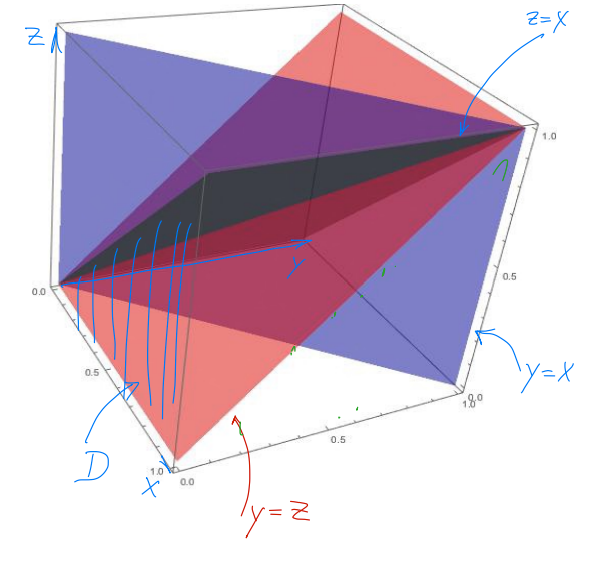
\includegraphics[scale=0.8]{22025-05-19.png}
	\end{center}
\end{parag}
\begin{parag}{Exemple 4}
	Trouver le volume de la région $E \subset \mathbb{R}^{3}$ entre les plans $x =  0,  y = 0, z= 0$ et $2x + 3y - z =  6$.\\
	Donc déjà, on a $4$ plans, ce qui nous donnera dans notre cas un triangle. On cherche donc les arrêtes de se triangle (l'intérsection de deux plans ensemble) on a:
	\begin{align*} z =  0 \implies 2x + 3y = 6 \implies y =  2 -\frac{2}{3}x \end{align*}
	On a donc ensuite l'intersection de tout les plans:
	\begin{align*} x = 0, y = 0, z = 2x + xy - 6 \implies -6 \end{align*}
	On a donc:
	\begin{align*} E = \{0 < x < 3, 0 < y < 2- \frac{2}{3}x, 2x + 3y - 6 < z < 0\} \end{align*}
	Pouruoi dans ce sens? étant donnée que notre plan se trouve en dessous de 0, il est forcémment borné supérieurement par ce dernier.\\
	Si on calcule donc le volume:
	\begin{align*} 
		V &= \int\int\int_E 1 dxdydz = \int_0^3dx \int_0^{2 - \frac{2}{3}x}dy \int_{2x + 3x - 6}^0\\
		  &= \int_0^3dx \int_0^{2 - \frac{2}{3}x}(-2x - 3y + 6)dy\\
		  &= \int_0^3dx \int_0^{2 - \frac{2}{3}x}(-2x - 2y + 6)dy =  \int_0^3dx (-2xy - \frac{3}{2}y^2 + 6y) \mid_0^{2 - \frac{2}{3}x}\\
		  &= \int_0^3 (-2x(2 - \frac{2}{3}x)- \frac{3}{2}(2- \frac{2}{3}x)^2 + 6(2 - \frac{2}{3}x))dx \\
		  &= \int_0^3 -4x + \frac{4}{3}x^2 - 6 + 4x - \frac{2}{3}x^2 + 12 - 4x dx\\
		  &= \int_0^3 - 4x + \frac{2}{3}x^2 + 6 dx = -2x^2 + \frac{2}{9}x^3 + 6x \mid_0^3 =  6
	\end{align*}
\end{parag}



\subsection{Changement de variables dans une intégrale multiple}
\begin{theoreme}

Soit $E \subset \mathbb{R}^{n}$ un sous-ensemble ($\overline{E}$ compact); $\psi: E \to \mathbb{R}^{n}$ telle que $\psi \in C'\left(E\right)$ et $\psi: E \to \psi\left(E\right)$ est bijective ($J_\psi\left(\overline{u}\right)$ est invertible $\forall \overline{u} \in E$).\\
Soit $f: \overline{D} = \overline{\psi\left(E\right)} \to \mathbb{R}$ une fonction continue.\\
Alors:
\begin{align*} \int_D f(\overline{x})d\overline{x} = \int_E f(\psi(\overline{u})) \cdot  \left|\det J_{\psi} (\overline{u})\right|d\overline{u} \end{align*}
\end{theoreme}
\begin{parag}{Example 0}
    On prends $f\left(x,y\right) = 1 =  f\left(u, v\right)$.\\
    Soit donc:
    \begin{align*} \psi (u, v) =  \begin{pmatrix} 3u \\ 2b \end{pmatrix}  = \begin{pmatrix} x \\ y \end{pmatrix} \text{ de classe } C^1 \end{align*}
    \begin{align*} J_\psi (u, v) = \begin{pmatrix} 3 & 0 \\ 0 & 2 \end{pmatrix}  \implies \left|\det J_\psi \left(u, v\right)\right|= 6 \end{align*}
    
\end{parag}
\begin{parag}{Exemple 5}
	Soit $f\left(x,y\right) =  x^2$, $D =  \{\left(x,y\right) \in \mathbb{R}^{2}; 0 < x <1, -x < y < x\} \bigcup \{\left(x, y\right) \in \mathbb{R}^{2}: 1 < x < 2, x - 2 < y < 2 - x\}$.\\
	On calcule l'intégrale:
	\begin{align*} 
		\int \int_D f(x, y) dxdy =  \int_0^1 dx \int_{-x}^x x^2 dy + \int_1^2dx \int_{x-2}^{2-x}x^2dx
	\end{align*}
	Ou alors:
	\begin{align*} 
		\begin{cases}
		    u 2
		\end{cases} \implies
		E =  
		\begin{cases}
			(u, v) :  0 < u < 2\\ 0 < v < 2
		\end{cases} =
	\begin{cases}
	    x = \frac{1}{2}(u + v)\\ y =  \frac{1}{2}(u-v) 
	\end{cases}
	\end{align*}
	On a donc pour la jacobienne:
	\begin{align*} J_{\psi(u, v)} =  \begin{pmatrix} \frac{1}{2} &- \frac{1}{2} \\\frac{1}{2}  & \frac{1}{2} \end{pmatrix}  \implies \det J_{\psi (u, v)} =  \frac{1}{2}\end{align*}
	Ceux qui nous donne lorsqu'on calcule l'intégrale (attention à ne pas oublié le facteur du déterminant):
	\begin{align*} \int\int_D x^2dxdy =  \int\int_E (\frac{1}{2}(u + v))^2 \cdot  \frac{1}{2}dudv\\
		&= \int_0^2 dv \int_0^2 (\frac{1}{8}(u + v)^2)du\\
		\int_0^2 dv (\frac{1}{24}(u + v)^3\mid_0^2)\\
		&= \int_0^2 \frac{1}{24}((v + 2)^3 - v^3) dv\\
		&=  \frac{1}{24}\frac{1}{4} ((v + 2)^4 - v^4)\mid_0^2\\
		&= \frac{7}{3}
	\end{align*}
\end{parag}



\lecture{26}{2025-05-21}{Examen final approche}{}


\begin{parag}{Application: changement de variable polaire}
    \begin{align*} \psi \left(r, \phi\right) =  
        \begin{cases}
            x =  r \cos \phi\\
            y =  r \sin \phi
        \end{cases} \mathspace \mathspace \psi : \mathbb{R}_+ \times [ 0, 2\pi [ \to \mathbb{R}^{2} \setminus \left\{0\right\}
    \end{align*}
    avec $\psi$ qui est bijective\\
        On a donc pour la jacobienne:
        \begin{align*}
            J_{\phi}\left(r, \phi\right) =  \begin{pmatrix} \cos \phi & -r\sin \phi \\ \sin\phi & r\cos\phi \end{pmatrix}  \implies \det J_{\psi \left(r, \phi\right)} =  r \left(\cos^2\phi + \sin^2\phi\right) =  r
        \end{align*}

    \begin{center}
        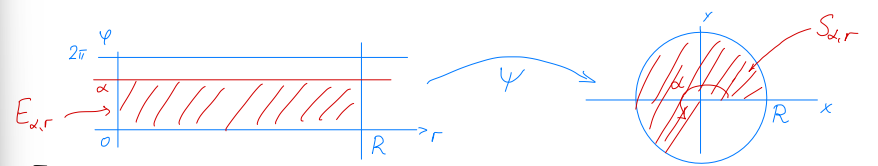
\includegraphics[scale=0.7]{12025-05-21.png}
    \end{center}
\end{parag}
\begin{parag}{Exemple 1}
    On cherche l'aire du secteur circluaire $S_{\alpha, r}$ d'angle $\alpha$ et de rayon $R$:
    \begin{center}
        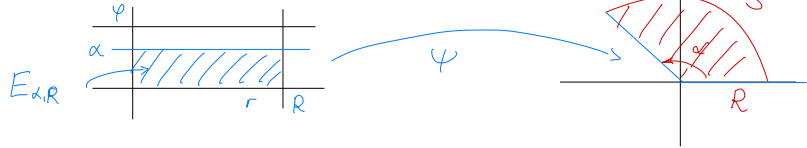
\includegraphics[scale=0-7]{22025-05-21.png}
    \end{center}
    On a donc:
    \begin{align*} A_{\alpha, r} =  \int\int_S 1 dxdy =  \int_0^\alpha d\phi \int_0^R \left| \det \psi_{r, \phi}\right|dr\\
        = \int_0^\alpha d\phi \int_0^R r dr =  \alpha \frac{1}{2} r^2\mid_0^R =  \frac{1}{2}R^2 \alpha
    \end{align*}
    Si $\alpha = 2\pi \implies $ l'aire du disque du rayon $R$ est:
    \begin{align*} A_{2\pi, R} =  \frac{1}{2} R^2 \cdot  2\pi =  \pi R^2 \end{align*}
    
\end{parag}
\begin{parag}{Exercice}
    L'aire du disque de rayon $1$ en coordonnées cartesiennes.
    \begin{align*} D =  \left\{\left(x, y\right) \in \mathbb{R}^{2}: x^2 + y^2 \leq 1\right\} \end{align*}
    On a donc l'intégrale qui est donnée par:
    \begin{align*} 
        A =  \int_{-1}^1 dx \int_{-\sqrt{1 - x^2}}^{\sqrt{1 - x^2}}1 dy =  \int_{-1}^1 2 \sqrt{1 - x^2}dx
    \end{align*}
    Ensuite on peut poser le changement de variable $x \sin t$. On utilisera aussi le fait que notre fonction est paire afin de calculer ``qu'une seule fois'' l'intégrale comme ceci:
    \begin{align*} 4 \int_0^2 \sqrt{1-x^2}dx \end{align*}
\end{parag}

\subsubsection{Conclusion: changement de variable polaires}


\begin{parag}{Cas important: Coordonnées polaires}
    \begin{align*} G \left( r, \phi\right) =  
        \begin{cases}
            r  \cos \phi =  x\\
            r \sin \phi =  y
        \end{cases}
    \end{align*}
    \begin{center}
        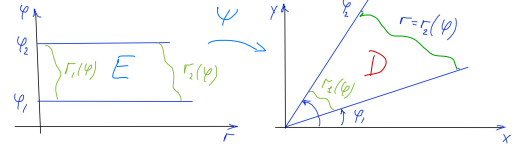
\includegraphics[scale=0.8]{32025-05-21.png}
    \end{center}
\end{parag}
\begin{parag}{Exemple}
    soit $f\left(x, y\right) = \sqrt{a^2 - x^2 - y^2}$ avec $a > 0$, $D$ est une boucle de lemmiscate de Bernouilli (1694):
    \begin{align*} \left(x^2 + y^2\right)^2 =  a^2\left(x^2 - y^2\right) \;\; x > 0 \end{align*}
    Si on chercher maintenant à le placer en coordonnées polaires:
    \begin{align*} 
        r^4 =  a^2\left(r^2\cos^2\phi - r^2 \sin^2 \phi\right) =  a^2 r^2 \cos 2\phi\\
        \iff r^2 =  a^2 \cos 2 \phi \implies \cos 2 \phi \geq 0
    \end{align*}
    Et donc:
    \begin{align*} 
        \cos 2 \phi > 0 \implies - \frac{\pi}{2} < 2\phi < \frac{\pi}{2} \\
        \implies - \frac{\pi}{4} \leq \phi \leq \frac{\pi}{4} \\
        \frac{3\pi}{4}< \phi < \frac{5\pi}{4} \; \; x <0
    \end{align*}
    On a donc finalement:
    $r =  a \sqrt{\cos 2 \phi}$ avec $- \frac{\pi}{4} \leq \phi \leq \frac{\pi}{4}$ qui est l'équation d'une boucle de la lemmiscate. \\
    Si on prends les deux ``maximum'', $\phi = \pm \frac{\pi}{4} \implies r = 0$ et ensuite $\phi =  0 \implies r = a$, on a donc finalement pour l'ensemble:
    \begin{align*} 
        E =  \left\{-\frac{\pi}{4} < \phi < \frac{\pi}{4}, 0 < r < a\sqrt{\cos 2 \phi} \right\}
    \end{align*}
        \begin{center}
            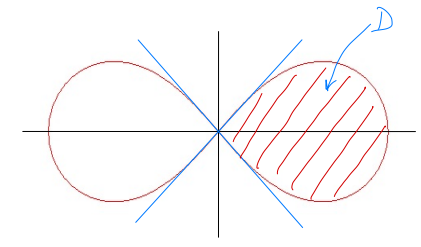
\includegraphics[scale=0-8]{42025-05-21.png}
        \end{center}
        On a donc avec un changement de variable:
        \begin{align*} 
            \int\int_D \sqrt{a^2 - x^2 - y^2} dxdy &= \int\int_E \sqrt{a^2-r^2} \underbrace{r}_{\left|\det J\right|}dr d\phi\\
            \int_{-\frac{\pi}{4}}^{\frac{\pi}{4}}d\phi \int_0^{a\sqrt{\cos 2\phi}}\sqrt{a^2 - r^2} rdr
        \end{align*}
        On voit ici qu'on peut juste faire un changement de variable $u = a^2 - r^2$ ce qui au vu du $r$ qui ``depasse'' de la racine va se simplifier:
        \begin{align*} 
            -\frac{1}{2}\int_0^{a\sqrt{\cos 2\phi}}\sqrt{a^2 - r^2}d\left(a^2 - r^2\right)\\ 
            &=  -\frac{1}{2} \cdot  \frac{2}{3} \left(a^2 - r^2\right)^{\frac{3}{2}}\mid_{0}^{a\sqrt{\cos 2\phi}}\\ 
            &= - \frac{1}{3}\left(a^2 - a^2 \cos 2 \phi\right)^{\frac{3}{2}} + \frac{1}{3}a^3
        \end{align*}
        Donc si on essaie de simplifier  tout ça:
        \begin{align*} 
            \left(1-\cos 2 \phi\right)^{\frac{3}{2}} =  \left(-\cos^2\phi + \sin^2\phi\right)^{\frac{3}{2}} = 2^{\frac{3}{2}}\left(\sin^2\phi\right)^{\frac{3}{2}} =  2^{\frac{3}{2}}\left|\sin\phi\right|^{3}
        \end{align*}
        Et donc on peut intégrer:
        \begin{align*} 
            \int_{-\frac{\pi}{4}}^{\frac{\pi}{4}} \left( - \frac{1}{3} 2^{\frac{3}{2}}a^3 \left|\sin \phi\right|^3 + \frac{1}{3}a^3\right) d\phi\\
            &=  \frac{1}{3}a^3 \left(\frac{\pi}{4} + \frac{\pi}{4}\right) - \frac{1}{3}a^3 2^{\frac{3}{2}}\int_{-\frac{\pi}{4}}^{\frac{\pi}{4}}\left| \sin\phi\right|^3 d\pih \\
            &= \frac{\pi}{6}a^3 - \frac{1}{3}a^3 2^{\frac{3}{2}}\cdot 2 \int_0^{\frac{\pi}{4}} \sin^3 \phi d \phi
        \end{align*}
        \begin{align*} 
            \int_0^{\frac{\pi}{4}} \sin^3 \phi d\phi &=  \int_0^{\frac{\pi}{4}}\left(-1 \cos^2\phi\right)d\left(-\cos\phi\right) \\
                                                     &=  \frac{1}{3} \cos^3\phi - \cos\phi \mid_0^{\frac{\pi}{4}} \\
                                                     &=  \frac{1}{3}\left(\frac{1}{\sqrt{2}}\right)^3 - \frac{1}{\sqrt{2}} - \frac{1}{3} + 1\\
            \frac{2}{3} + \frac{1}{\sqrt{2}}\left(\frac{1}{6} - 1\right) &=  \frac{2}{3}  - \frac{5}{6\sqrt{2}}
        \end{align*}
        Et donc si on remet tout ça dans notre intégrale en haut (qui comment par $\frac{\pi}{6}$)
        \begin{align*} 
            \int\int =  \frac{\pi a^3}{6} - \frac{a^3 \cdot  2^{\frac{3}{2}} \cdot  2}{3} \left(\frac{2}{3} - \frac{5}{6\sqrt{2}}\right) 
        \end{align*}
\end{parag}

\begin{parag}{Exemple 3}
    Soit $f\left(x, y\right) =  xy$ avec $D =  \left\{ \left(x + 1\right)^2 + y^2 \leq 1 , y \geq \frac{x}{\sqrt{3}}\right\}$\\
On voit en premier lieu que notre ensemble à une condition qui ressemble à un disque donc on peut essayer d'utiliser un changement de variable:
\begin{align*} 
    r^2\cos^2\phi + 2r\cos\phi + 1 + r^2\sin^2\phi \leq 1 &\implies r^2 + 2r\cos\phi \leq 0\\
    t + 2\cos\phi \leq 0 &\implies r \leq -2\cos\phi \implies \cos\phi < 0\\
                         &\implies \frac{\pi}{2} < \phi < \frac{3\pi}{2}
\end{align*}
Si on prends maintenant la deuxième condition avec un changement de variable polaire:
\begin{align*} 
    y \geq \frac{x}{\sqrt{3}} &\implies r \sin \phi \geq \frac{r \cos \phi}{\sqrt{3}}\\
                              &\implies \sin\phi \geq \frac{\cos \phi}{\sqrt{3}}\\
\end{align*}
Ce qui nous donne deux cas, soit $\sin\phi > 0, \cos \phi < 0 \implies \frac{\pi}{2} < \phi < \pi$. ou alors $\sin \phi < 0, \cos\phi < 0 \implies \tan \phi < \frac{1}{\sqrt{3}}$.\\
et donc si on développe pour $\phi$ on a:
\begin{align*} 
    \tan \phi =  \frac{1}{\sqrt{3}} \implies \phi =  \frac{\pi}{6} + \pi k \implies \pi < \phi < \frac{7}{6}\pi
\end{align*}
On a donc notre ensemble qui est:
\begin{align*} 
    E =  \left\{\frac{\pi}{2} < \phi < \frac{7}{6}\pi, 0 < r < -2 \cos\phi\right\}
\end{align*}
Il reste plus qu'a intégrer:
\begin{align*} 
    \int\int_D xy dxdy &=  \int_{\frac{\pi}{2}}^{\frac{7\pi}{6}}d\phi \int_0^{-2\cos\phi}r^2 \cos\phi s\sin\phi r dr\\
                       &= \int_{\frac{\pi}{2}}^{\frac{7\pi}{6}}d\phi \left(\frac{1}{4}r^4 \cos \phi \sin\phi\right)\mid_0^{-2\cos\phi}\\
                       &= 4 \int_{\frac{\pi}{2}}^{\frac{7\pi}{6}}\cos^5\phi\sin\phi d\phi\\
                       &= -4 \int_{\frac{\pi}{2}}^{\frac{7\pi}{6}}\cos^5\phi d \cos \phi\\ 
                       &= - \frac{4}{6}\cos^6 \phi \mid_{\frac{\pi}{2}}^{\frac{7\pi}{6}} =  \cos \frac{7\pi}{6} =  -\cos \frac{\pi}{6} =  -\frac{\sqrt{3}}{2}
\end{align*}
\begin{center}
    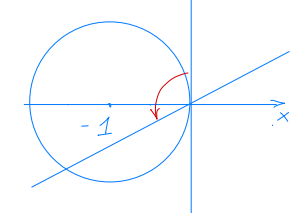
\includegraphics[]{52025-05-21.png}
\end{center}
\begin{subparag}{Coordonnées cartesiennes}
    \begin{align*} 
        D =  \left\{\left(x + y\right)^2  + y^2 \leq 1, y \geq \frac{x}{\sqrt{3}} \right\}
    \end{align*}
    On a donc:
    \begin{align*} 
        y =  \frac{x}{\sqrt{3}} \implies \left(x + 1\right)^2 + \frac{x^2}{3} =  1 \\
        \implies \frac{4}{3}x^2 + 2x + 1 =  1 = \begin{cases} x =  0 \\ \frac{4}{3}x =  -2 \end{cases}
    \end{align*}
    Ce qui implique donc que:
    \begin{align*} 
         \begin{cases}
             x =  0\\ x = -\frac{2}{3}
         \end{cases} , \; y =  - \frac{\sqrt{3}}{2}
    \end{align*}
    On a donc pour l'autre condition:
    \begin{align*} 
        y^2 \leq 1 - \left(x + 1\right)^2 \implies -\sqrt{1 - \left(x + 1\right)^2} <y< \sqrt{1 - \left(x + 1\right)^2}
    \end{align*}
    Et cela sur $D_1$.
    \begin{align*} 
        \frac{x}{\sqrt{3}} < y < \sqrt{1 - \left(x + 1\right)^2}
    \end{align*}
    Si on met donc l'union de nos deux ensemble ensemble:

    \begin{align*} 
    D =  \left\{-2 \leq x \leq -\frac{3}{2}, - \sqrt{1 - \left(x + 1\right)^2} < y < \sqrt{1 - \left(x + 1\right)^2}\right\}\\
    \bigcap \left\{\frac{-3}{2}<x<0, \frac{x}{\sqrt{3}} < y < \sqrt{1 - \left(x + 1\right)^2}\right\}
    \end{align*}
    On peut ensuite intégrer sur cette ensemble.
\end{subparag}
\end{parag}

\subsubsection{Coordonnées sphérique}
\begin{parag}{Coordonnée sphérique}
    \begin{align*} 
        G \left( r, \theta, \phi\right) = \begin{cases} x =  r \sin\theta \cos\phi\\ y =  r\sin\phi \sin \theta\\ z = r\cos\theta\end{cases}
    \end{align*}
    On a  donc $G:  ] 0, \infty [ \times [ 0, \pi ] \times [ 0, 2\pi [ \to \mathbb{R}^{3}\setminus \left\{\overline{0}\right\} $\\
    On peut donc calculer la jacobienne qui est donné par:
    \begin{align*} 
        J_{G\left(r, \theta, \phi\right)} = \begin{pmatrix} \sin \theta\cos\phi & r\cos\theta\cos\phi & -r\sin\theta\cos\phi \\ \sin\theta\sin\phi & r\cos\theta\sin\phi & r\sin\theta\cos\phi \\ \cos\theta & -r\sin\theta & 0 \end{pmatrix} 
    \end{align*}
    Je passe les calculs avec la règle de Sarrus mais  on obtient:
    \begin{align*} 
        \left|\det J_{G\left(r, \theta, \phi\right)}\right| =  \left|r^2\cos^2\theta\sin\theta + r^2\sin^3\theta\right| =  \left|r^2\sin\theta\right| \mathspace 0 < \theta < \pi
    \end{align*}

\end{parag}


\begin{parag}{Exemple, Volume d'une boule de rayon $a > 0$}
    On a donc pour l'ensemble:
    \begin{align*} 
        E =  \left\{0 < r < a, 0 < \theta < \pi, 0 < \phi < 2\pi\right\}
    \end{align*}
    On a donc pour le volume:

    \begin{align*} 
        V &=  \int\int\int_{B\left(\overline{0}, a\right)} 1 dxdydz &= \int_0^{2\pi}d\phi\int_0^\pid\theta\int_0^a r^2\sin\theta dr\\
          &= \int_0^{2\pi}d\phi\int_0^\pi\sin\theta d\theta \cdot  \int_0^a r^2 dr\\
          &= 2\pi\left(-\cos\theta\right)\mid_0^\pi \cdot  \frac{1}{3}r^3 \mid_0^a \\
          &= 2\pi\left(1 + 1\right) \cdot  \frac{1}{3}a^3 =  \frac{4}{3}\pi a^3 
    \end{align*}
\end{parag}

\subsubsection{Application: masse totale d'un objet solide}
\begin{parag}{Masse total d'un objet de solide de densité donnée}
    \begin{align*} 
        M = \int\int\int_V \rho \left(x, y, z\right) dxdydz
    \end{align*}
    est la masse totale du volume $V$ avec la densité $\rho\left(x,y, z\right)$
\end{parag}
\begin{parag}{Exemple}
    Trouver la masse totale d'un secteur sphérique:
    \begin{align*} 
        S = \left\{x > 0, y > 0, z > 0, x^2 + y^2 + z^2 < a^2\right\}
    \end{align*}
    Avec la fonction de densité $\rho \left(x, y, z\right) =  x^2 + y^2$.\\
    On a va donc comme on l'a fait juste avant, effectuer une changement de variable en coordonnées sphérique ce qui nous donne donc:
    \begin{align*} 
        E =  \left\{0 < r < a, 0 < \theta < \frac{\pi}{2}, 0 < \phi < \frac{\pi}{2}\right\}
    \end{align*}
    Ce qui nous donne donc:
    \begin{align*} 
        M &=  \int\int\int_S \left(x^2 + y^2\right) dxdydz = \int_0^{\frac{\pi}{2}}d\ph\iint_0^{\frac{\pi}{2}}d\theta \int_0^a r^2 \sin^2 \theta \underbrace{r^2 \sin \theta}_{\left|\det J\right|}dr\\
         &=  \int_0^{\frac{\pi}{2}} d\phi \int_0^{\frac{\pi}{2}}\sin^3\theta d \theta \int_0â r^4 dr\\
         &= \frac{\pi}{2}\int_0^{\frac{\pi}{2}}\left(\cos^2\theta - 1\right)d\cos \theta \cdot \frac{1}{5}r^5\mid_0^a = \frac{\pi}{2}\left(\frac{1}{3}\cos^3\theta - \cos \theta\right)\mid_0^{\frac{\pi}{2}} \cdot  \frac{1}{5}a^5\\
         &= \frac{\pi a^5}{10}\left(-\frac{1}{3} + 1\right) =  \frac{\pi a^5}{15}
    \end{align*}

\end{parag}
\begin{parag}{Question du jour}
    \begin{align*} f\left(x, y\right) =  2x + 3y \end{align*}
    Avec
    \begin{align*} D = \left\{\left(x, y\right) \in \mathbb{R}^{2}: x < 0, y > 0, 1 < x^2 + y^2 < 4\right\} \end{align*}
    Alors $\int\int_D f\left(x, y\right) dxdy $ vaut?\\
    Alors en premier lieu on peut changer en coordonnée polaire:
    \begin{align*} 
        D = \left\{\left(r, \phi\right): r \cos \phi < 0, r \sin \phi > 0, 1 < r^2 < 4\right\}
    \end{align*}
    On écrit notre fonction en coordonnée
    \begin{align*} 
        f\left(r \phi\right) =  2r\cos\phi + 3r\sin\phi
    \end{align*}
    Comme $x < 0$ et que $y > 0$ on sait donc que  $\phi > \frac{\pi}{2}$ et  aussi que $\phi < \pi$ comme on a $1 < r^2 < 4 \implies 1 < r < 2$ (on s'occupe pas du négatif).

\end{parag}










\subsubsection{Rappel: Méthode d'intégration des fonctions de plusieurs variables}
\lecture{27}{2025-05-26}{Dernier cours???}{}


\begin{parag}{Théorème de Fubini $\implies$ changement d'ordre d'intégration}
   \begin{center}
       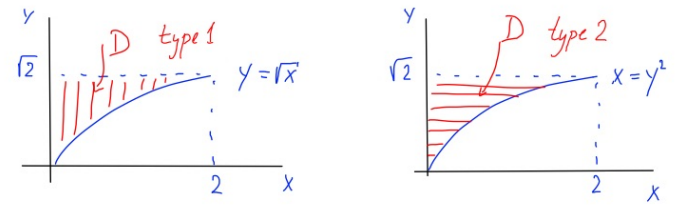
\includegraphics[scale=0.8]{12025-05-26.png}
   \end{center}
   Qui nous donne:
   \begin{align*} 
       \int_0^2dx\int_{\sqrt{x}}^{\sqrt{2}}f\left(x, y\right) dy =  \int_{0}^{\sqrt{2}}dy\int_0^{y^2}f\left(x, y\right)dx
   \end{align*}
\end{parag}
\begin{parag}{L'additivité de l'intégrale $\implies$ Division du domaine d'intégration}
    \begin{center}
        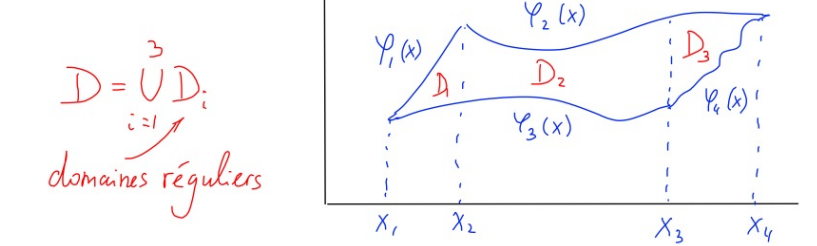
\includegraphics[scale=0.8]{22025-05-26.png}
    \end{center}
    Il faut diviser le domaine en réunion et utiliser l'additivité de l'intégrale.
    
    
\end{parag}
\begin{parag}{Changement de variable}
    
    \begin{theoreme}
    Soit $E \subset \mathbb{R}^{n} $ un sous-ensemble, $\overline{E}$ est compact, $\psi: E \to \mathbb{R}^{n}$ telle que $\psi \in C^1\left(E\right)$, et $\psi: E \to \psi\left(E\right) = D$ bijective. Soit $f : \overline{D}  = \overline{\psi\left(E\right)} \to \mathbb{R}$ un fonction continue. Alors:
    \begin{align*} \int_D f\left(\overline{x}\right) =  \int_E f\left(\psi\overline{u}\right)\left|\det J_{\psi\left(\overline{u}\right)}\right|d\overline{u} \end{align*}
    \end{theoreme}
        \begin{center}
            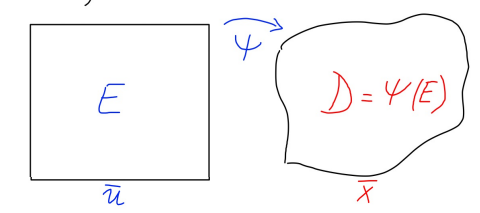
\includegraphics[scale=0.8]{32025-05-26.png}
        \end{center}
\end{parag}
\begin{parag}{Coordonnées sphérique}
    \begin{align*} 
        G\left(r, \theta, \phi\right) =  
        \begin{cases}
            x =  r \sin \theta \cos \phi\\
            y = r \sin \theta \sin \phi\\
            z =  r \cos \theta
        \end{cases}
    \end{align*}
    \begin{center}
        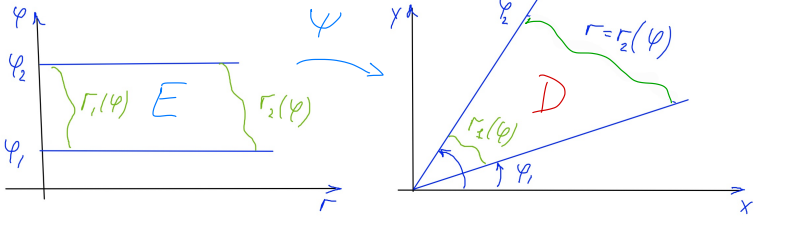
\includegraphics[scale=0.6]{42025-05-26.png}
    \end{center}
    \begin{align*} \left|\det J_{G\left(r, \theta, \phi\right)}\right| = r^2\s\in\theta \end{align*}
\end{parag}
\begin{parag}{Exemple}
    Le volume d'un ellipsoide $\left\{\left(x, y, z\right) \in \mathbb{R}^{3}: \frac{x^2}{a^2} + \frac{y^2}{b^2} + \frac{z^2}{c^2} \leq 1\right\}$.
    On pose le changement de variable:
    \begin{align*} 
        \begin{cases}
            x =  au\\
            y = bv\\
            z = cw
            \end{cases} &\implies \left\{\left(u, v, w\right)\in \mathbb{R}^{3}: u^2 + v^2 + w^2 \leq 1\right\} \implies J_{H\left(u, v, w\right)} = \begin{pmatrix} a & 0 & 0 \\ 0 & b & 0 \\ 0 & 0 & c \end{pmatrix} \\
                        &\implies \left|\det J_H\right| = \left|abc\right| 
    \end{align*}
    \begin{center}
        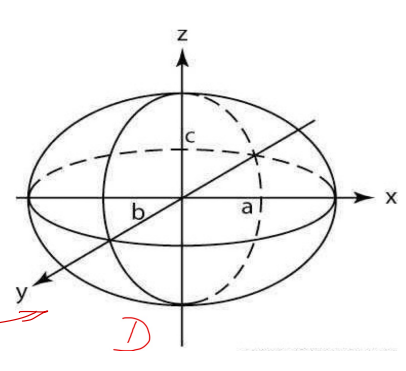
\includegraphics[scale=0.7]{62025-05-26.png}
    \end{center}
    
    Donc ici on en premier lieu, le changement de variable polaire (on passe de l'ellipsoide à une sphère) et ensuite de la sphère à un pavé:
    \begin{align*} 
        J_{H \mathring G} = J_{H\left(G\right)} \cdot  J_G = \left| \underbrace{\det J_{H\left(G\right)}}_{abc}\right| \cdot  \left|\underbrace{\det J_G}_{r^2 \sin \theta}\right| = abcr^2\sin\theta
    \end{align*}
    On a donc notre volume:
    \begin{align*}
        V =  \int_0^{2\pi}d\phi \int_0^\pi d \theta \int_0^1 abcr^2\sin\theta dr =  abc\int_0^{2\pi} d \phi \int_0^\pi \sin \theta d \theta \int_0^1 r^2 dr =  abc \frac{4}{3}\pi
    \end{align*}
\end{parag}
\begin{parag}{Coordonnées cylindriques}
    \begin{align*} 
    G\left(r, \theta, z\right) =     \begin{cases}
            x =  r \cos\phi\\
            y =  r \sin \phi\\
            z =  z
        \end{cases}
    \end{align*}
    On a donc notre fonction $G: [0, \infty[ \times [ 0, 2\pi[ \times \mathbb{R} \to \mathbb{R}^{3}  $, Je passe les details pour la jacobienne mais son déterminant est donnée par:
    \begin{align*} \det J_{G\left(r, \phi, z\right)} =  r \end{align*}
    \begin{center}
        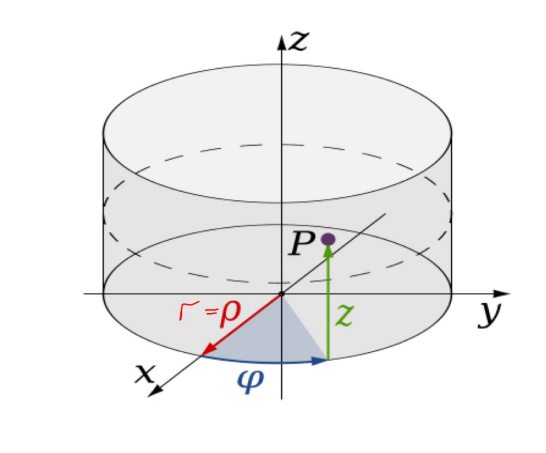
\includegraphics[scale=0.4]{72025-05-26.png}
    \end{center}
    
\end{parag}
\begin{parag}{Exemple}
    Trouver le volume du domaine $D$ avec les frontières:
    \begin{align*} 
        \begin{cases}
            x^2 + y^2 + z^2 =  2za, a > 0\\
            x^2 + y^2 =  z^2
        \end{cases}
    \end{align*}
    Qui contient $\left(0, 0, a\right)$. Donc ici comme on a des $x^2 + y^2$ mais dans $\mathbb{R}^{3}$ (sans le $+ z^2$) les coordonnés cylindrique sont utiles:
    \begin{align*} 
        \begin{cases}
            r^2 + z^2 - 2za = r^2 + z^2 - 2za + a^2 = a^2\\
            r^2 =  z^2
        \end{cases} \implies 
        \begin{cases}
            r^2 + \left(z-a\right)^2 =  a^2\\
            r = z, z \geq 0\\
            r =  -z, z \leq 0
        \end{cases}
    \end{align*}
    On a ici donc une sphère de rayon $a$ qui est centré en $\left(0, 0, a\right)$. Pour ce qui est de la deuxième équation, comme $r = z$, on a le rayon du cercle qui est égal à la hauteur, plus la hauteur plus le rayon du cercle augment (on parle pas de la sphère ici). Est donc on a un \important{cône}.\\
    On cherche donc l'intersection qui se trouve en $r = z$:
    \begin{align*} 
        a^2 &= r^2 + \left(r-a\right)^2 \\
           0 &=2r^2 + -2ra\\
             &= 2r\left(r-a\right) \implies r = a= z
    \end{align*}
    On a ici donc le cercle de rayon $a$ dans le plan $a = z$.\\
    On a donc notre volume qui se calcule avec la somme d'un demi sphère de rayon $a$ et d'un cône $r = z$ coupé par $0 < z < a$.\\
    Donc la démi sphère est donné par:
    \begin{align*} \frac{1}{2}\frac{4}{3}\pi a^3 =  \frac{2}{3}\pi a^3 \end{align*}
    On cherche donc maintenant le volume du cône (qui a donc un angle de $\frac{\pi}{4}$ (vu qu'on a $z = r$) et une hauteur de $a$):
    Si on écrit l'ensemble:
    \begin{align*} 
        D =  \left\{0 < z < a, 0 < \phi < 2\pi, 0 < r < z\right\}
    \end{align*}
    \begin{align*} 
        V &= \int_0^{2\pi}d\phi \int_0^a dz \int_0^z r dr = 2\pi \int_0^a \left(\frac{1}{2}r^2\mid_0^z\right)dz\\
          &= \pi \int_0^a z^2 dz\\
          &= \frac{1}{3}\pi z^3\mid_0^a = \frac{1}{3}\pi a^3
    \end{align*}
    On a donc le volume total:
    \begin{align*} V = \frac{2}{3}\pi a^3 + \frac{1}{3}\pi a^3 =  \pi a^3 \end{align*}
\end{parag}
\begin{parag}{Géométrique de changement de variables}
   \begin{framedremark}
        Dans le changement de variables sphériques et cylindriques, une coordonnée cartesienne est de la forme spéciale \important{$z$}. Mais selon la géométrique du domaine et la fonction donnée, on peut choisir une autre coordonnée cartesienne d'avoir cette forme spéciale, par exemple $y$
   \end{framedremark} 
   \begin{center}
       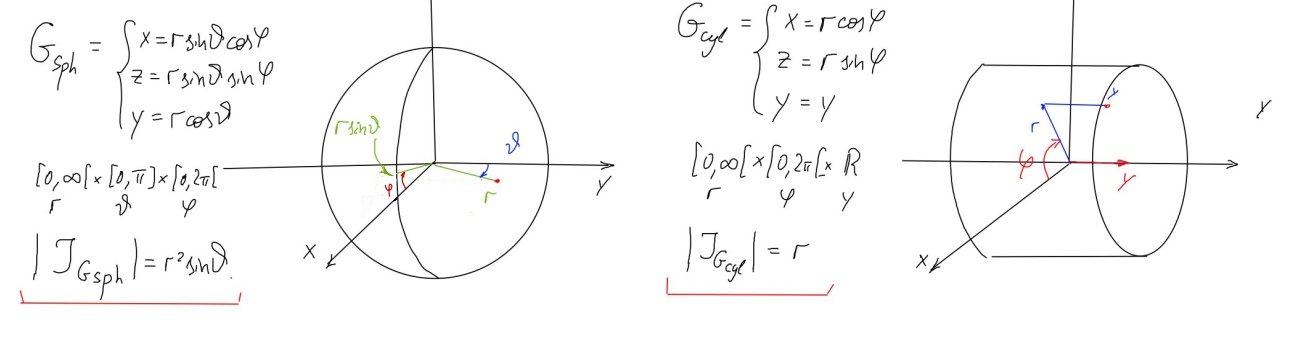
\includegraphics[scale=0.6]{82025-05-26.png}
   \end{center}
\end{parag}


\begin{parag}{Exemple}
    \begin{align*} 
        \int\int\int_E e^y dxdydz, \; \; E = \left\{\left(x, y, z\right) \in \mathbb{R}^{3}: x^2 +z^2 \leq 4, -\sqrt{x^2 + z^2} < y < \sqrt{x^2 + z^2}\right\}
    \end{align*}
   On a donc avec le changement de coordonnées cylindrique:
   \begin{align*} 
   \begin{cases}
       x =  r\cos \phi\\
       y = r\sin \phi\\
       z = z
   \end{cases}
   \end{align*}
   On a donc notre ensemble qui change:
   \begin{align*} 
       E =  \left\{{\left(r, \phi, z\right): 0 < \phi < 2\pi, 0 < r < 2, -r < y < r^2\right\}
   \end{align*}
   Il nous reste plus qu'à intégrer (avec le déterminant de la jacobienne):
   \begin{align*} 
       \int_0^{2\pi}d \phi \int_0^2 dr \int_{-r}^{r^2}e^y \cdot  r dy
   \end{align*}
\end{parag}
\chapter{Fin du cours, Révision}

\section{Intégrale}
\begin{parag}{(1)}
    \begin{align*} 
        \int\int_D \arcsin \left(\frac{y}{\sqrt{x^2 + y^2}}\right)dxdy \\
        D = \left\{\left(x, y\right) \in \mathbb{R}^{2}: x \geq 0, y \leq 0, 1 \leq x^2 + y^2 \leq 9\right\}
    \end{align*}
    On voit ici qu'on a deux cercle (plus grand que $1$ et plus petit que $9$) et qu'on prends donc dans un seul cadran (celui ou $x \geq 0$ et $y \leq 0$.\\
    On va utiliser les coordonnées polaires: $D =  \left\{\left(r, \phi\right): -\frac{\pi}{2} < \phi < 0, 1 < r < 3\right\}$  on obtient donc:
    \begin{align*} 
        \int_{-\frac{\pi}{2}}^{0}d \phi \int_1^3 \arcsin\left(\frac{r \sin\phi}{r}\right)\cdot r dr &= \int_{-\frac{\pi}{2}}^0d \phi \int_1^3 \phi r dr\\
                                                                                                    &= \frac{1}{2}\phi^2\mit_{-\frac{\pi}{2}}^0 \cdot  \frac{1}{2}r^2\mid_1^3 = -\frac{1}{2}\pi^2
    \end{align*}
\end{parag}
\begin{parag}{(2)}
    \begin{align*} \int\int\int_V z^2 dxdydz \end{align*}
    Avec comme domaine:
    \begin{align*} V =  \left\{\left(x, y, z\right): x <y, x^2 + y^2 < 4, 0 < z < \left(x^2 + y^2\right)^{\frac{1}{4}}\right\} \end{align*}
    Donc on a ici un cercle centré en $\left(0, 0, 0\right)$ de rayon $2$ coupé par la droite $x =  y$ et nous prenons ce qu'il y a au dessus de cette droite, le demi cercle au dessus de la droite $x = y$.\\
    Pour ce qui est du $z$ c'est pas très clair donc on préfère ``l'ignorer'' pour l'instant.\\
    Donc par changement de variable on a:
    \begin{align*} 
        V =  \left\{\left(r, \phi, z\right): \frac{\pi}{4} < \phi < \frac{5\pi}{4}, 0 < r < 2, 0 < z < \sqrt{r}\right\}
    \end{align*}
    On a donc si on réécrit l'intégrale:
    \begin{align*} 
        \int\int\int_V z^2 dxdydz &= \int_{\frac{\pi}{4}}^{\frac{5\pi}{4}}d\phi \int_0^2 dr \int_0^{\sqrt{r}}z^2 r dz\\
                                  &= \phi \mid_{\frac{\pi}{4}}^{\frac{5\pi}{4}} \cdot  \int_0^2 r \frac{1}{3}z^3 \mid_0^{\sqrt{r}}dr\\
                                  &= \pi \cdot  \frac{1}{3}\int_0^2 r^{\frac{5}{3}}dr = \frac{\pi}{3}\cdot  \frac{2}{7} \cdot  r^{\frac{7}{2}}\mid_0^2\\
                                  &= \frac{16\pi}{21}\sqrt{2}
    \end{align*}
\end{parag}
\begin{parag}{(3)}
    \begin{align*} \int\int\int_D \end{align*}
    Avec le domaine 
    \begin{align*} 
        D =  \left\{\left(x, y\right)\in \mathbb{R}^{2}: -1 \leq y \leq 1, y^2 \leq x \leq 1\right\}
    \end{align*}
    On a donc ici la fonction $y =  x^2$ renvérsé (sur le côté) de $x =  y^2$ et $x =  \left(-y\right)^2$:
    \begin{align*} 
        \int_{-1}^1 dy \int_{y^2}^1 \sin y \cos x dx &=\int_{-1}^1dy\left(\sin y\left( \sin 1 - \sin\left(y^2\right)\right)
    \end{align*}
    Néanmoins la fonction $\sin\left(y^2\right)$ n'a pas de primitive de fonction usuelle donc on va simplement essayer avec un autre type. Donc ici ça sera le $x$ qui varie entre deux nombre et le $y$ qui lui entre des fonctions de $x$:
    \begin{align*} 
        D =  \left\{\left(x, y \right) \in \mathbb{R}^{2}: 0 < x < 1, -\sqrt{x} < y <\sqrt{x}\right\}
    \end{align*}
    Si on réécrit donc notre intégrale on a:
    \begin{align*} 
        \int_0^1 dx \int_{-\sqrt{x}}^{\sqrt{x}}\sin y \cos x dx &= \int_0^1dx \left(\cos x \left(-\cos y\right)\mid_{-\sqrt{x}}^{\sqrt{x}}\\
                                                                &= \int_0^1 \cos x \left(-\cos \sqrt{x} + \cos \left(-\sqrt{x}\right)\right)dx\\
                                                                &= 0
    \end{align*}
    Ici on voit ici qu'on a $f\left(x, y\right) =  \sin y \cos x$ mais on voit que cette dernière est pair: $f\left(x, -y\right) = \sin$ (pas eu le temps mais ducoup ca faisait 0)
\end{parag}
\begin{parag}{Question 23}
    Soit $D =  \left\{\left(x, y\right)\in \mathbb{R}^{2}: x \geq -1, \left|y\right| \leq 1 - x\right\}$. On demande la forme de cette ensemble.\\
    \begin{subparag}{Réponse}
        Ici on peut remarque deux truc important, on a la ``réciproque'' (pas formellement mais à peu près) de la fonction $f\left(x\right) =  \left|x\right|$. Ensuite on a fonc les max se trouve $ x =  -1$ et si on évalue pour $y$: $\left|y\right| = 1 - - 1$ ce qui nous donne donc $\left|y\right|= 2 \implies  y =\pm 2$. donc on à un triangle avec les point $\left(-1, \pm 2\right)$. Ensuite on a donc le maximum pour $x =  1$ et donc $y =  0$. 
    \end{subparag}
\end{parag}

\begin{parag}{Question 24}
    L'intégrale $\int_{\frac{\pi}{4}}^{\frac{\pi}{2}}d \phi \int_o^{\frac{1}{\sin \phi}}r dr$ exprime l'aire d'un(e):
    \begin{itemize}
        \item Secteur circulaire
        \item Triangle
        \item Rectangle
        \item Tranche d'un cercle
    \end{itemize}
    \begin{subparag}{Réponse}
        Donc déjà on a des coordonnés polaires avec donc $D = \left\{\left(\phi, r\right): \frac{\pi}{4} < \phi < \frac{\pi}{2}, 0 < r < \frac{1}{\sin \phi}\right\}$. On a donc $0 < r < \frac{1}{\sin \phi}$ ce qui est une droite
    \end{subparag}
\end{parag}













\end{document}

